%  LaTeX support: latex@mdpi.com
%  For support, please attach all files needed for compiling as well as the log file, and specify your operating system, LaTeX version, and LaTeX editor.

%=================================================================
\documentclass[sensors,article,submit,pdftex,moreauthors]{Definitions/mdpi}
% For posting an early version of this manuscript as a preprint, you may use "preprints" as the journal. Changing "submit" to "accept" before posting will remove line numbers.

%--------------------
% Class Options:
%--------------------
%----------
% journal
%----------
% Choose between the following MDPI journals:
% accountaudit, acoustics, actuators, addictions, adhesives, adolescents, aerobiology, aerospace, agriculture, agriengineering, agrochemicals, agronomy, ai, aichem, aieng, aimater, aimed, aipa, air, aisens, algorithms, allergies, alloys, amh, analog, analytica, analytics, anatomia, anesthres, animals, antibiotics, antibodies, antioxidants, applbiosci, appliedchem, appliedmath, appliedphys, applmech, applmicrobiol, applnano, applsci, aquacj, architecture, arm, arthropoda, asc, asi, astronautics, astronomy, atmosphere, atoms, audiolres, automation, axioms, bacteria, batteries, bdcc, beverages, biochem, bioengineering, biologics, biology, biomass, biomechanics, biomed, biomedicines, biomedinformatics, biomimetics, biomolecules, biophysica, bioresourbioprod, biosensors, biosphere, biotech, birds, blockchains, bloods, blsf, brainsci, breath, buildings, cancers, carbon, cardio, cardiogenetics, cardiovascmed, catalysts, cells, ceramics, challenges, chemengineering, chemistry, chemosensors, chemproc, children, chips, cimb, civileng, cleantechnol, climate, clinbioenerg, clinpract, clockssleep, cmd, cmtr, coasts, coatings, colloids, colorants, commodities, complexities, complications, compounds, computation, computers, condensedmatter, conservation, constrmater, cosmetics, covid, crops, cryo, cryptography, crystals, csmf, ctn, culture, curroncol, cyber, dairy, data, ddc, dentistry, dermato, dermatopathology, designs, devices, dhi, diabetology, diagnostics, dietetics, digital, disabilities, diseases, diversity, dna, drones, dynamics, earth, ebj, ecm, ecologies, edm, eesp, electricity, electrochem, electronicmat, electronics, encyclopedia, endocrines, energies, eng, engproc, entomology, entropy, environments, environremediat, epidemiologia, epigenomes, esa, est, fermentation, fibers, fintech, fire, fishes, fluids, foods, forecasting, forensicsci, forests, fossstud, foundations, fractalfract, fuels, future, futureinternet, futurepharmacol, futurephys, futuretransp, galaxies, gases, gastroent, gastrointestdisord, gastronomy, gels, genes, geographies, geohazards, geomatics, geometry, geosciences, geotechnics, geriatrics, germs, glacies, grasses, green, greenhealth, gucdd, hardware, hazardousmatters, healthcare, hearts, hemato, hematolrep, hep, heritage, higheredu, highthroughput, horticulturae, hospitals, hydrobiology, hydrogen, hydrology, hydropower, hygiene, idr, iic, ijem, ijerph, ijgi, ijmd, ijms, ijns, ijom, ijpb, ijt, ijtm, ijtpp, ime, immuno, informatics, information, infrastructures, inorganics, insects, instruments, inventions, iot, j, jaestheticmed, jal, jcdd, jcm, jcp, jcrm, jcs, jcto, jdad, jdb, jdream, jemr, jeta, jfb, jfmk, jgbg, jgg, jimaging, jlpea, jmahp, jmmp, jmms, jmp, jmse, jne, jnt, jof, joi, joitmc, joma, jop, joptm, jor, jox, jpbi, jphytomed, jpm, jsan, jtaer, jvd, jzbg, kidneydial, kinasesphosphatases, knowledge, labmed, laboratories, lae, land, life, lights, limnolrev, lipidology, liquids, livers, logics, logistics, lubricants, lymphatics, machines, macromol, magnetism, magnetochemistry, make, marinedrugs, materials, materproc, mathematics, mca, measurements, medicina, medicines, medsci, membranes, merits, metabolites, metals, meteorology, methane, metrics, metrology, micro, microarrays, microbiolres, microelectronics, micromachines, microorganisms, microplastics, microwave, minerals, mining, mmphys, modelling, molbank, molecules, mps, msf, mti, multimedia, muscles, nanoenergyadv, nanomanufacturing, nanomaterials, ncrna, ndt, network, neuroglia, neuroimaging, neurolint, neurosci, nitrogen, notspecified, nursrep, nutraceuticals, nutrients, obesities, occuphealth, oceans, ohbm, onco, optics, oral, organics, organoids, osteology, oxygen, pandemics, parasites, parasitologia, particles, pathogens, pathophysiology, pediatrrep, pets, pharmaceuticals, pharmaceutics, pharmacoepidemiology, pharmacy, philosophies, photochem, photonics, phycology, physchem, physics, physiologia, plants, plasma, platforms, pollutants, polymers, polysaccharides, populations, poultry, powders, precipitation, precisoncol, preprints, proceedings, processes, prosthesis, proteomes, psf, psychiatryint, psychoactives, purification, quantumrep, quaternary, qubs, radiation, rdt, reactions, realestate, receptors, recycling, regeneration, remotesensing, reports, reprodmed, resources, rheumato, rjpm, robotics, rsee, ruminants, safety, sci, scipharm, sclerosis, seeds, sensors, separations, sexes, shi, signals, sinusitis, siuj, skins, smartcities, sna, societies, software, soilsystems, solar, solids, spectroscj, sports, standards, stats, std, stratsediment, stresses, surfaces, surgeries, suschem, sustainability, symmetry, synbio, systems, tae, targets, taxonomy, technologies, telecom, test, textiles, thalassrep, therapeutics, thermo, timespace, tomography, toxics, toxins, tph, transplantology, transportation, traumacare, traumas, tri, tropicalmed, universe, urbansci, uro, vaccines, vehicles, venereology, vetsci, vibration, virtualworlds, viruses, vision, waste, water, welding, wem, wevj, wild, wind, women, world, zoonoticdis

%---------
% article
%---------
% The default type of manuscript is "article", but can be replaced by: 
% abstract, addendum, article, benchmark, book, bookreview, briefcommunication, briefreport, casereport, changes, clinicopathologicalchallenge, comment, commentary, communication, conceptpaper, conferenceproceedings, correction, conferencereport, creative, datadescriptor, discussion, entry, expressionofconcern, extendedabstract, editorial, essay, erratum, fieldguide, hypothesis, interestingimages, letter, meetingreport, monograph, newbookreceived, obituary, opinion, proceedingpaper, projectreport, reply, retraction, review, perspective, protocol, shortnote, studyprotocol, supfile, systematicreview, technicalnote, viewpoint, guidelines, registeredreport, tutorial,  giantsinurology, urologyaroundtheworld
% supfile = supplementary materials

%----------
% submit
%----------
% The class option "submit" will be changed to "accept" by the Editorial Office when the paper is accepted. This will only make changes to the frontpage (e.g., the logo of the journal will get visible), the headings, and the copyright information. Also, line numbering will be removed. Journal info and pagination for accepted papers will also be assigned by the Editorial Office.

%------------------
% moreauthors
%------------------
% If there is only one author the class option oneauthor should be used. Otherwise use the class option moreauthors.

%---------
% pdftex
%---------
% The option pdftex is for use with pdfLaTeX. Remove "pdftex" for (1) compiling with LaTeX & dvi2pdf (if eps figures are used) or for (2) compiling with XeLaTeX.

%=================================================================
% MDPI internal commands - do not modify
\firstpage{1} 
\makeatletter 
\setcounter{page}{\@firstpage} 
\makeatother
\pubvolume{1}
\issuenum{1}
\articlenumber{0}
\pubyear{2026}
\copyrightyear{2026}
%\externaleditor{Firstname Lastname} % More than 1 editor, please add `` and '' before the last editor name
\datereceived{ } 
\daterevised{ } % Comment out if no revised date
\dateaccepted{ } 
\datepublished{ } 
%\datecorrected{} % For corrected papers: "Corrected: XXX" date in the original paper.
%\dateretracted{} % For retracted papers: "Retracted: XXX" date in the original paper.
%\doinum{} % Used for some special journals, like molbank
%\pdfoutput=1 % Uncommented for upload to arXiv.org
%\CorrStatement{yes}  % For updates
%\longauthorlist{yes} % For many authors that exceed the left citation part
%\IsAssociation{yes} % For association journals

\usepackage{graphicx}
% Image files: project root (./) or figures/ subfolder; use exact basenames from disk
\graphicspath{{./}{figures/}}
\usepackage{multirow}
\usepackage{amsmath,amssymb,amsfonts,amsthm,mathrsfs}
\usepackage{textcomp,manyfoot}
\usepackage{booktabs}
\usepackage{array}
\usepackage{tabularx}
\usepackage{caption}
\usepackage{placeins}
\usepackage{float}
\usepackage{pifont}
\usepackage{microtype}
% Keep deferred floats from piling up after the bibliography
\setcounter{topnumber}{4}
\setcounter{bottomnumber}{4}
\setcounter{totalnumber}{10}
\renewcommand{\textfraction}{0.10}
\renewcommand{\topfraction}{0.90}
\renewcommand{\bottomfraction}{0.90}
\renewcommand{\floatpagefraction}{0.80}
\usepackage{algorithm,algorithmicx,algpseudocode}
\usepackage{listings}
\newcolumntype{Y}{>{\raggedright\arraybackslash}X}
\setlength{\headheight}{20pt}
\usepackage{makecell}
% L column type provided by mdpi.cls

% Title options --- keep exactly one \Title{...} active (comment/uncomment others):
% Alt.\ 2 (AMI + edge--fog):\quad \Title{Federated Kernel SVMs with Differential Privacy for Edge--Fog Cooperative Intrusion Detection over Advanced Metering Infrastructure}
% Alt.\ 3 (compact methods-first):\quad \Title{Cooperative Intrusion Detection in Smart Meter Networks Using Federated Kernel SVMs with Differential Privacy}
\Title{Federated Kernel SVMs with Differential Privacy for Cooperative Intrusion Detection in Smart Meter Networks}

% Insert each corresponding author's ORCID iD (https://orcid.org/). Leave empty if unavailable.
\newcommand{\orcidauthorA}{}

\Author{
Farrukh Aslam Khan$^{1,*}$,
Tayyab Rehman$^{2}$,
Noshina Tariq$^{3}$ and
Jalal Almuhtadi$^{4}$
}

\AuthorNames{Farrukh Aslam Khan, Tayyab Rehman, Noshina Tariq and Jalal Almuhtadi}

\address{
$^{1}$ Center of Excellence in Information Assurance, DSR, King Saud University, Riyadh 11653, Saudi Arabia; fakhan@ksu.edu.sa\\
$^{2}$ Department of Information Engineering, Computer Science, and Mathematics, University of L'Aquila, 67100 L'Aquila, Italy; tayyab.rehman@graduate.univaq.it\\
$^{3}$ Department of Artificial Intelligence and Data Science, National University of Computer and Emerging Sciences, Islamabad 44000, Pakistan; noshina.tariq@isb.nu.edu.pk\\
$^{4}$ Department of Computer Science, College of Computer and Information Sciences (CCIS), King Saud University, Riyadh, Saudi Arabia; jalal@ksu.edu.sa
}

\corres{Correspondence: fakhan@ksu.edu.sa}

\abstract{Advanced Metering Infrastructure (AMI) connects millions of endpoints to IP networks, elevating risks from denial-of-service traffic, false data injection (FDI), and reconnaissance while requiring strong privacy, low communication overhead, and robustness to heterogeneous client traffic. This work presents an edge--fog--cloud intrusion detection framework that integrates federated radial-basis-function kernel support vector machines (SVMs), Gaussian differential privacy (DP) with composed budgets, diversity-aware federated averaging (DA-FedAvg), a fog-level stacked ensemble, and SHapley Additive exPlanations (SHAP) for interpretable triage. A cooperative design applies edge-side scoring to volumetric threats and fog-side inference on cross-meter score vectors without centralising raw flows. On CICIDS2017, CICIoT2023, and Edge-IIoT, accuracies reach up to 99.10\%, 98.07\%, and 96.34\% with ROC-AUC up to 0.998, 0.995, and 0.979 under centralised or independent and identically distributed (IID) federated training. Zone-aware Dirichlet partitions quantify statistically heterogeneous (non-IID) client effects, including about 83\% federated accuracy versus an 87\% centralised ceiling on a CICIoT2023-profile replay at concentration 0.5, together with FedProx, clustered aggregation, and Platt scaling for probability calibration under DP. The results establish a reproducible, multi-objective reference for privacy-preserving cooperative detection in smart meter networks.
}

\keyword{Federated intrusion detection; differential privacy; smart grid; smart meter networks; federated learning; edge computing; fog computing; ensemble learning; support vector machines; non-IID data}

\begin{document}

% ═══════════════════════════════════════════════════════════════════════
% Section 1. Introduction
% ═══════════════════════════════════════════════════════════════════════
\section{Introduction}\label{sec1}

The rapid digitalization of energy systems has made Smart Grids (SG) a cornerstone of modern infrastructure, integrating digital communication with physical power distribution to enable real-time metering, automated demand response, and remote load management through Advanced Metering Infrastructure (AMI)~\cite{zhang2024federated}. While this transformation brings significant operational benefits, it simultaneously creates a vast and continuously expanding cyber attack surface. AMI nodes (the smart meters deployed at millions of consumer premises) communicate over standard IP-based protocols and are increasingly targeted by adversaries launching denial-of-service (DoS) floods, injecting falsified energy readings to corrupt billing and grid-state estimation, and conducting reconnaissance to identify exploitable entry points~\cite{ciaramella2025method, ajiboye2024privacy, tariq2024fog}. Industrial and logistics-adjacent IoT settings exhibit closely related wireless-layer threats (notably jamming and spoofing); recent work couples fog computing with federated learning to detect such families under privacy constraints~\cite{rehman2024ffl} and surveys federated intrusion-detection countermeasures for those attack classes~\cite{rehman2024fl_jamming_survey}. Broader security-analytics research further shows that hybrid classical and Transformer models can strengthen context-aware detection pipelines~\cite{gulzaib2025inmic}, a design perspective that informs interpretable multi-model IDS stacks. The consequences extend beyond service disruption: a coordinated attack on AMI infrastructure can destabilize grid operations, cause cascading failures, and undermine public trust in critical energy services. Network flow statistics observed at meters and concentrators provide a distributed, privacy-sensitive measurement stream over AMI communications, which aligns intrusion detection on those features with network-level sensing contexts relevant to operational monitoring research.

The urgency of this problem is underscored by the scale of AMI deployment (projected to exceed 1.3 billion connected meters globally by 2030) and by the increasing sophistication of attacks targeting operational technology. Existing Intrusion Detection Systems (IDS) are ill-equipped to meet these demands. Cloud-centralised architectures require raw consumer data to be transmitted to remote servers, creating privacy violations and unacceptable detection latency~\cite{hamdi2025investigating, buyuktanir2025federated}. Federated Learning (FL) offers a privacy-preserving alternative by sharing only model parameters, yet its performance degrades significantly under the non-IID traffic conditions inherent to real SG deployments, where urban and rural substations observe fundamentally different attack patterns~\cite{alshamasi2025federated, fdla_dc_microgrids}. Compounding this, most FL-IDS frameworks deploy a single detection model per node, which is insufficient for the diverse and evolving AMI threat landscape, and provide no operator-interpretable explanation of their decisions, impeding timely incident response~\cite{naeem2025classification, hamdi2025hybrid}. There is therefore a compelling need for a framework that characterises and manages competing objectives (privacy, accuracy, communication cost, and client heterogeneity) rather than treating them as independent add-ons, and that delivers \textit{transparent} federated IDS evidence under non-IID conditions together with operator-facing interpretability.

This paper proposes a multi-objective edge--fog--cloud IDS for SG AMI. The framework positions the deployment as an operating point on a constrained trade-off surface (Section~\ref{r3}): it enables collaborative training without raw traffic exchange, quantifies privacy loss through $(\varepsilon,\delta)$-DP and composition, minimises uplink relative to raw-flow centralisation, and employs heterogeneity-aware aggregation including diversity-aware federated averaging (DA-FedAvg). Hierarchical cooperative detection structures inference into (i)~edge-side \textit{local certainty} from margin-based scores and (ii)~fog-side \textit{global correlation inference} over cross-client score vectors, implemented with emulated latency bounds (Section~\ref{sec:casestudy}).

The framework pursues: (O1)~privacy-preserving collaboration with formal DP (including composition) and no raw AMI data leaving the edge; (O2)~systematic characterisation of federated IDS under heterogeneous clients (Dirichlet sweeps, PCAP and protocol replay), plus partial mitigation via fine-tuning, DA-FedAvg, FedProx, and regional aggregation, with explicit reporting of residual gaps; (O3)~interpretable multi-family detection via fog ensemble and SHAP.

The principal contributions are:
\begin{itemize}
  \item \textit{Multi-objective federated IDS framework:} A principled formulation of the privacy--accuracy--communication--heterogeneity trade-off (Section~\ref{r3}), instantiated by a three-tier architecture with DP noise, composed budgets, DA-FedAvg, and fog--cloud ensemble learning.
  \item \textit{Non-IID as scientific evidence:} Controlled Dirichlet stress tests, $\alpha$ sweeps, mitigations, and reproducible protocol replay that document \textit{how} federated IDS accuracy scales with heterogeneity severity, serving as benchmark methodology, not merely a negative result (Section~\ref{r7}).
  \item \textit{Hierarchical cooperative detection:} A two-level paradigm that combines local certainty at the edge with collective correlation at the fog for volumetric versus distributed stealthy threats, with emulated timing (Section~\ref{sec:casestudy}).
  \item \textit{DA-FedAvg and empirical positioning:} Client weights scaled by local label-entropy diversity with renormalisation ($\lambda{=}0$ recovers size-weighted FedAvg); validated in ablation (Section~\ref{r7}), alongside deep baselines, Byzantine aggregators, and SHAP-guided feature reduction.
\end{itemize}

Table~\ref{tab:related_work_ids} positions the proposed framework against representative prior work across four dimensions: formal DP/non-IID handling (D1), fog ensemble architecture (D2), operator interpretability (D3), and identified open future directions (D4). The remainder of this paper is organised as follows: Section~\ref{r2} reviews related work; Section~\ref{r3} presents the proposed framework; Sections~\ref{r5}--\ref{r6} describe the experimental setup and methodology; Section~\ref{r7} reports results; Section~\ref{sec:casestudy} presents the end-to-end case study; Sections~\ref{r9}--\ref{r10} discuss findings and conclude.

\begin{figure}[!htbp]
  \centering
  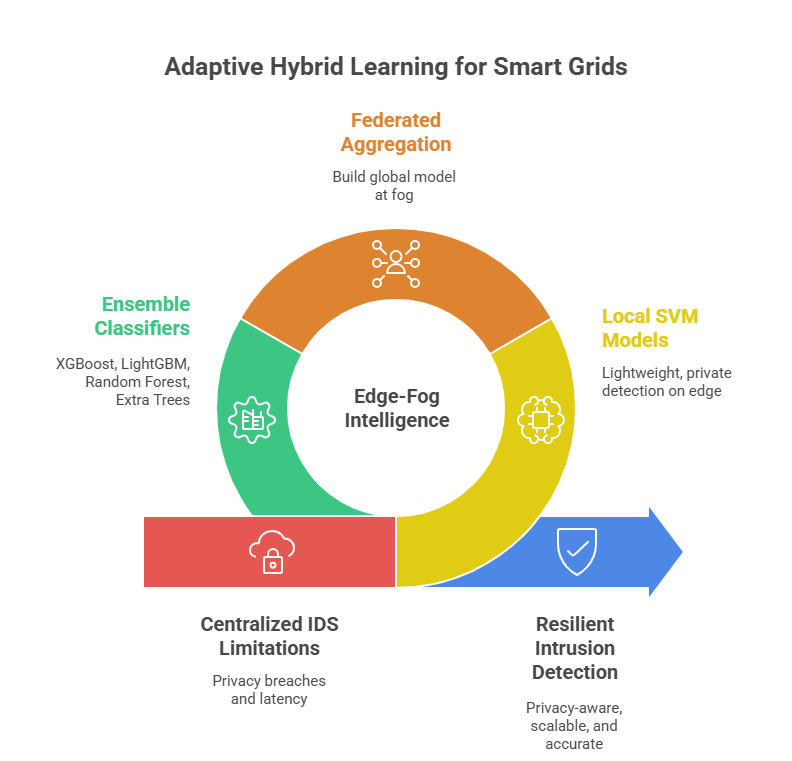
\includegraphics[width=0.95\linewidth,keepaspectratio]{An Adaptive Hybrid Learning Framework.png}
  \caption{An adaptive hybrid learning framework.}
  \label{fig:adaptive_hybrid}
\end{figure}

% ═══════════════════════════════════════════════════════════════════════
% Section 2. Related work
% ═══════════════════════════════════════════════════════════════════════
\section{Related Work}\label{r2}

This review covers IDS research published between 2017 and 2025 in IEEE, ACM, Elsevier, and Springer venues, targeting smart grid, industrial IoT, and AMI security. From an initial pool of 147 papers, 21 were retained using the following criteria. \textit{Inclusion:} (i)~primary focus on network-level intrusion detection; (ii)~evaluation on a labelled benchmark; (iii)~relevance to distributed or privacy-constrained deployment. \textit{Exclusion:} (i)~purely anomaly-detection without classification; (ii)~physical-layer methods without network-layer features; (iii)~preprints without peer review; (iv)~works focused solely on malware classification. Table~\ref{tab:inclusion_exclusion} presents the full search protocol, inclusion/exclusion criteria, and screening funnel; the retained works are organised below into four thematic tracks.

\begin{table}[H]
\caption{Literature search protocol: inclusion/exclusion criteria and screening funnel (initial pool: 147 papers; final retained: 21).~\label{tab:inclusion_exclusion}}
	\begin{adjustwidth}{-\extralength}{0cm}
		\begin{tabularx}{\fulllength}{>{\raggedright\arraybackslash}p{1.5cm} >{\raggedright\arraybackslash}X >{\centering\arraybackslash}p{1.6cm}}
\toprule
\textbf{ID} & \textbf{Criterion} & \textbf{Papers} \\
\midrule
\multicolumn{2}{l}{\textit{Inclusion (all must hold)}} & \\[1pt]
I1 & Primary focus on network-level intrusion detection or multi-class attack classification & \\
I2 & Evaluation on a labelled network-flow benchmark (CICIDS, Edge-IIoT, KDD, or equivalent) & \\
I3 & Relevance to distributed, privacy-constrained, or edge--fog deployment & 58 \\
\midrule
\multicolumn{2}{l}{\textit{Exclusion (any one sufficient to reject)}} & \\[1pt]
E1 & Purely anomaly detection without class labels & $-$14 \\
E2 & Physical/signal-layer only; no network-layer features & $-$12 \\
E3 & Preprint or workshop paper without peer review & $-$7 \\
E4 & Endpoint malware classification only; no network IDS component & $-$4 \\
\midrule
\multicolumn{2}{l}{\textit{Screening funnel}} & \\[1pt]
& Initial database hits (IEEE, ACM, Elsevier, Springer; 2017--2025) & 147 \\
& After title/abstract screen & 83 \\
& After full-text inclusion check (I1--I3) & 58 \\
& \textbf{Final retained (meets I1--I3, fails no E1--E4)} & \textbf{21} \\
\bottomrule
\end{tabularx}
	\end{adjustwidth}
\end{table}


\noindent\textit{Federated and privacy-preserving IDS.} FL has attracted significant interest as a mechanism for privacy-sensitive IDS in SG environments. Husnoo et al.~\cite{husnoo2023feddisc} proposed FedDiSC, combining gradient quantisation with deep autoencoders to distinguish disturbances from cyberattacks at low communication cost, though generalisation under non-IID traffic remains limited. Liang et al.~\cite{liang2023intrusion} fine-tune DNNs at AMI data concentrators without exposing user data, but risk gradient divergence under heterogeneous distributions. Hossain et al.~\cite{hossain2023modbus} apply FL to Modbus RS-485 smart meter communications, preserving confidentiality while detecting protocol-level anomalies; the system is however protocol-specific and not cross-validated. Aashmi et al.~\cite{aashmi2023federated} propose a fully decentralised FL-IDS with no central repository, enabling proactive anomaly defence at the cost of known convergence instability. At the governance level, Hernández-Ramos et al.~\cite{HernandezRamos2024} survey FL-IDS configurations and document open challenges around client poisoning and non-IID data, while Latif et al.~\cite{Latif2025} examine secure aggregation strategies and note that energy-constrained AMI settings remain largely unsolved. Islam et al.~\cite{blockchain_sg_2024} augment FL with blockchain smart contracts for tamper-resistant aggregation, though the consensus overhead is incompatible with real-time AMI constraints. Across these works, a common gap is the absence of formal $(\varepsilon,\delta)$-DP analysis and adaptive aggregation strategies for non-IID client distributions.

\noindent\textit{Fog and edge computing architectures.} Alsirhani et al.~\cite{Alsirhani2025} propose a fog-integrated ensemble that reduces raw data transfer and achieves robust detection, but relies on manual feature engineering that limits generalisability. A three-tier hierarchical FL system for DDoS detection~\cite{SpringerOpen2024} improves data locality at the cost of inter-tier synchronisation bottlenecks and high communication overhead. Mohan et al.~\cite{Mohan2024} develop a rule-driven distributed IDS for SCADA substations using DNP3 semantic rules; the system demonstrates substation deployability but cannot handle unknown attacks or generalise beyond DNP3. These architectures confirm the operational value of edge--fog distribution but fall short in ensemble diversity and non-IID robustness.

\noindent\textit{Deep learning and graph-based classifiers.} Ciaramella et al.~\cite{Ciaramella2025} apply an explainable DL-CNN to network traffic, improving operator interpretability at the expense of feasibility on AMI-tier hardware. Aljohani et al.~\cite{Aljohani2024} present a DL-based intrusion detection and mitigation system with attack localisation; resource consumption renders it impractical on embedded AMI nodes. Ma et al.~\cite{Ma2025} describe AS-TBR, a spatiotemporal model for AMI anomaly detection with robust feature extraction but complex runtime tuning requirements. Graph-based approaches, including BS-GAT~\cite{Wang2025}, which constructs behaviour-similarity graphs, and GraphKAN~\cite{Wu2025}, which combines graph attention with Kolmogorov--Arnold networks, demonstrate strong detection performance but lack FL integration and carry high computational cost. Transformer-based and LLM-augmented IDS~\cite{Transformers2024} report strong generalisation but are data-hungry, computationally expensive, and offer weak interpretability. Digital twin evaluation frameworks~\cite{DigitalTwin2024} enable realistic cyber-physical testing but require substantial engineering effort and suffer from synchronisation drift. Deep GraphSAGE enhancements~\cite{GraphSAGE2025} improve detection accuracy across multiple datasets but have not been extended to federated or edge settings.

\noindent\textit{Attack-specific detection for SG.} Wang et al.~\cite{fdla_dc_microgrids} propose a data-driven framework for FDI detection and localisation in DC microgrids, demonstrating that topology-aware features substantially improve accuracy. Liu et al.~\cite{pso_atgcn} present PSO-ATGCN, combining particle swarm optimisation with temporal graph convolution for dummy data injection detection, achieving strong temporal attack modelling. Both works are fully centralised and offer no privacy preservation. Alshamasi~\cite{Alshamasi2025} examines FL governance challenges in SG deployments, connecting FL to FDI and DDoS threat models. Hamdi~\cite{hamdi2025hybrid} investigates hybrid centralised-federated learning for IDS, demonstrating accuracy gains but providing no formal DP analysis. Liu and Pi~\cite{liu2017kernel} apply kernel SVM with game-theoretic models, showing multi-stage detection accuracy improvements in a static, non-federated setting.

\noindent\textit{Research gaps.} Table~\ref{tab:related_work_ids} maps each reviewed work across four dimensions (D1--D4). \textit{Dim-1 (Formal DP/non-IID):} Few FL-IDS works jointly publish formal $(\varepsilon,\delta)$-DP analysis, round-level composition, heterogeneity-aware aggregation, and measured non-IID stress tests on modern IoT benchmarks. \textit{Dim-2 (Fog ensemble):} Fog-level stacked ensembles fed by federated edge scores remain under-explored relative to single-model FL-IDS. \textit{Dim-3 (Interpretability):} Operator-facing SHAP attribution in an end-to-end federated IDS pipeline is still uncommon. \textit{Dim-4 (Future directions):} All reviewed works identify open problems including embedded benchmarking, SG-protocol evaluation, and personalised FL, which this work enumerates in Section~\ref{r10}. The contribution addresses all four dimensions as a principled multi-objective framework with explicit trade-off analysis, heterogeneity-aware aggregation (DA-FedAvg), and systematic non-IID characterisation.

\begin{table}[H]
\caption{Comparison of representative SG-IDS and FL-based intrusion detection works. Acc.\ reported as published; ``--'' not disclosed.~\label{tab:related_work_ids}}
	\begin{adjustwidth}{-\extralength}{0cm}
	{\footnotesize
		\begin{tabularx}{\fulllength}{%
  >{\raggedright\arraybackslash}p{0.9cm}%
  >{\raggedright\arraybackslash}p{2.0cm}%
  >{\raggedright\arraybackslash}p{1.5cm}%
  >{\raggedright\arraybackslash}X%
  >{\raggedright\arraybackslash}X%
  >{\raggedright\arraybackslash}X%
}
\toprule
\textbf{Ref.} & \textbf{Method} & \textbf{Dataset} & \textbf{Key Result} & \textbf{Limitation} & \textbf{Future Direction} \\
\midrule
\cite{husnoo2023feddisc}   & FL + autoencoder (FedDiSC)       & Power disturbance data   & Low comm.\ cost; disturbance vs.\ attack discrimination    & Non-IID sensitivity; small-scale              & Non-IID robustness; large-scale validation \\
\cite{liang2023intrusion}  & FL-DNN at AMI concentrators      & CICIDS2017               & Privacy-preserving AMI IDS; no raw data exposed            & Gradient divergence; heterogeneous dist.      & Heterogeneous FL; Modbus/DNP3 protocols \\
\cite{liu2017kernel}       & Kernel SVM + game theory         & KDD Cup~99               & Multi-stage detection; Acc.${\approx}$99\%                 & Static; no FL; no privacy                     & FL integration; real-time AMI deployment \\
\cite{hossain2023modbus}   & FL on Modbus RS-485              & Smart meter traffic      & Confidential protocol anomaly detection                    & Protocol-specific; binary only                & Multi-protocol; cross-domain generalisation \\
\cite{aashmi2023federated} & Decentralised FL-IDS             & NSL-KDD                  & No central repository; proactive anomaly defence           & Convergence instability; no DP                & DP integration; convergence stabilisation \\
\cite{Alsirhani2025}       & Fog-integrated ensemble          & CICIDS2017               & Reduced data transfer; robust fog detection                & Manual features; limited scalability          & Automated features; SG-protocol eval. \\
\cite{Mohan2024}           & Rule-driven IDS (DNP3)           & SCADA/DNP3 traffic       & Substation-deployable semantic detection                   & DNP3-only; no unknown-attack handling         & Unknown-attack generalisation; IEC~60870 \\
\cite{SpringerOpen2024}    & Three-tier hierarchical FL       & Simulated DDoS           & Improved data locality; tiered detection                   & Sync bottlenecks; high comm.\ overhead        & Async FL; lightweight aggregation \\
\cite{Ciaramella2025}      & Explainable DL-CNN               & CICIDS2017               & Operator interpretability; strong DL accuracy              & High compute; AMI-infeasible                  & Edge-deployable distilled models \\
\cite{Aljohani2024}        & DL-based IDMS + localisation     & Custom traffic           & Attack localisation; multi-family detection                & Resource-intensive; edge-infeasible           & Lightweight DL; FL integration \\
\cite{Ma2025}              & AS-TBR spatiotemporal model      & AMI sensor data          & Robust feature extraction; adaptive detection              & Complex tuning; gateway limits                & Embedded deployment; FL extension \\
\cite{Alshamasi2025}       & FL governance review             & Survey (FDI/DDoS)        & SG FL challenges and open problems documented              & No implementation; high overhead              & Personalised FL; lightweight governance \\
\cite{Latif2025}           & FL security / secure aggregation & Survey                   & Secure aggregation strategies surveyed                     & Latency at scale; heavy messaging             & Energy-constrained AMI FL \\
\cite{Wang2025}            & BS-GAT (graph attention IDS)     & CICIDS2017/2018          & Strong graph-based detection; behaviour similarity         & No FL; no privacy preservation                & FL-integrated graph IDS \\
\cite{Wu2025}              & GraphKAN (graph + KAN)           & NSL-KDD, UNSW-NB15       & High representation power; improved accuracy               & Complex training; edge-incompatible           & Federated GNN; model compression \\
\cite{Transformers2024}    & Transformer/LLM-augmented IDS    & Multiple benchmarks      & Strong generalisation across attack families               & Data-hungry; weak interpretability           & Lightweight Transformers; AMI edge \\
\cite{blockchain_sg_2024}  & Blockchain FL aggregation        & SG simulation            & Tamper-resistant FL; smart-contract aggregation            & Consensus overhead; real-time incompatible    & Off-chain aggregation; latency reduction \\
\cite{fdla_dc_microgrids}  & Data-driven FDI localisation     & DC microgrid testbed     & Topology-aware FDI; Acc.${\approx}$96\%                    & Fully centralised; no privacy                 & Federated extension; AC grid generalisation \\
\cite{pso_atgcn}           & PSO-ATGCN temporal graph conv.   & Power injection data     & Temporal attack modelling; dummy data injection            & Centralised; no privacy                       & Privacy-preserving FL; real-time SG \\
\cite{DigitalTwin2024}     & Digital twin testing             & SmartGridComm sim.       & Realistic cyber-physical evaluation                        & Engineering complexity; sync drift            & Lightweight DT; FL-integrated eval. \\
\cite{GraphSAGE2025}       & Deep GraphSAGE IDS               & CICIDS2017, UNSW-NB15    & Adaptable graph IDS; multi-dataset accuracy                & No FL/edge integration                        & Federated GraphSAGE; AMI protocol graphs \\
\cite{hamdi2025hybrid}     & Hybrid centralised-FL IDS        & CICIDS2017               & Accuracy gains over pure FL                                & No formal DP; limited non-IID handling        & RDP accounting; non-IID mitigation \\
\midrule
\multicolumn{6}{>{\raggedright\arraybackslash}p{\dimexpr\fulllength-2\tabcolsep\relax}}{%
\textbf{Proposed framework:} Fed.\ RBF-SVM + DA-FedAvg + Gaussian DP + fog ensemble + SHAP.
CICIDS2017: 99.10\%, CICIoT2023: 98.07\%, Edge-IIoT: 96.34\%.
Formal $(\varepsilon,\delta)$-DP; Stage~1 ${\approx}$20\,ms edge, Stage~2 ${\approx}$420\,ms fog;
Dirichlet non-IID; SHAP; lightweight 15-feature variant ($\Delta{=}{-}0.21\%$).} \\
\bottomrule
\end{tabularx}
	}
	\end{adjustwidth}
\end{table}

% ═══════════════════════════════════════════════════════════════════════
% Section 3. Proposed model
% ═══════════════════════════════════════════════════════════════════════
\section{Proposed Framework}\label{r3}

\subsection{System Overview and Threat Model}

The proposed framework is a three-tier intrusion detection framework designed to address the co-occurring challenges of privacy, non-IID data heterogeneity, and detection diversity in SG AMI deployments. As illustrated in Fig.~\ref{fig:architecture}, the framework operates across three tiers. At the \textit{edge} tier, $M$ smart meters each maintain a private local dataset $\mathcal{D}_m = \{(x_i, y_i)\}_{i=1}^{N_m}$, $x_i \in \mathbb{R}^d$, $y_i \in \{-1,+1\}$, and independently train local detection models without sharing any raw traffic. At the \textit{fog} tier, regional aggregators collect differentially private parameter updates from edge clients, apply diversity-aware federated averaging (DA-FedAvg; reduces to size-weighted FedAvg when the diversity coefficient $\lambda{=}0$), and maintain a globally refined model. At the \textit{cloud} tier, a stacked ensemble of four diverse classifiers is trained on aggregated edge-model decision scores to provide robust multi-family threat detection. No raw flow records leave the edge tier at any stage of the pipeline.

The threat model covers three adversarial scenarios: (i)~passive eavesdroppers intercepting transmitted model parameters; (ii)~active Byzantine clients submitting poisoned local updates to corrupt the global model; and (iii)~external attackers generating DoS/DDoS, FDI, and reconnaissance traffic on the AMI network.

\noindent\textit{Collusion and trust boundaries.} An \textit{honest majority} of edge clients and fog aggregators: if a coalition controls more than half of participating meters and colludes on malicious updates, no aggregation rule can guarantee correctness without additional authentication or hardware roots of trust. Passive colluding eavesdroppers who observe only differentially private releases receive limited information per round; their cumulative advantage still composes over rounds (Section~\ref{r3}). If secure aggregation (masked sums) is disabled, the fog coordinator can observe per-client updates and must be trusted accordingly. Collusion among a majority of fog nodes remains out of scope and is deferred to multi-aggregator architectures (Section~\ref{r10}).

\subsection{Problem Formulation and Trade-offs}\label{sec:problem_formulation}

The proposed framework treats AMI intrusion detection as a constrained multi-objective design problem. Let $\mathcal{A}$ denote detection quality (e.g.\ accuracy, F1, or ROC-AUC on a held-out evaluation partition), $\mathcal{P}$ a scalar privacy loss increasing with cumulative exposure (e.g.\ composed $\varepsilon_{\mathrm{tot}}$ from Table~\ref{tab:dp_composition}, or decreasing with noise scale $\sigma$ in Table~\ref{tab:dp_tradeoff}), and $\mathcal{C}$ communication cost (e.g.\ uplink bytes per round or total over $T$ rounds; contrast 336\,B per client per round here with multi-gigabyte raw-flow centralisation, Section~\ref{r3}). Design choices are organised along a conceptual scalar utility
\begin{equation}
\max \; U = \alpha\,\mathcal{A} - \beta\,\mathcal{P} - \gamma\,\mathcal{C},
\label{eq:utility}
\end{equation}
with non-negative coefficients $(\alpha,\beta,\gamma)$. \textit{Note:} the coefficients $(\alpha,\beta,\gamma)$ are \textit{not} jointly optimised or fitted from data in this paper--they are not estimated and Pareto-optimal solutions are not computed. Equation~\eqref{eq:utility} is an organising principle only: experiments in Section~\ref{r7} report \textit{slices} of the implied surface (e.g.\ varying $\sigma$ for fixed architecture, or non-IID severity for fixed $(\sigma,T)$), making trade-offs explicit for operators and regulators without claiming to optimise the surface itself.

\subsection{Design Principles}\label{sec:design_principles}

Four principles ground the implementation:
\begin{itemize}
  \item \textit{Privacy-by-design:} No raw flows leave the edge; Gaussian DP on released parameters; composition of budgets across $T$ documented (Tables~\ref{tab:dp_tradeoff}--\ref{tab:dp_composition}).
  \item \textit{Heterogeneity-aware learning:} Dirichlet stress tests and $\alpha$ sweeps; DA-FedAvg (Section~\ref{r3}); FedProx and zone-clustered models where applicable (Section~\ref{r7}).
  \item \textit{Distributed intelligence:} Edge autonomy (local SVM training and Stage~1 scoring) with fog coordination (DA-FedAvg, Stage~2 ensemble on score vectors), aligned with hierarchical cooperative detection.
  \item \textit{Interpretability as an operational requirement:} SHAP attribution and transparent scalar scores for triage, not post-hoc explanation only.
\end{itemize}

\begin{figure}[!htbp]
  \centering
  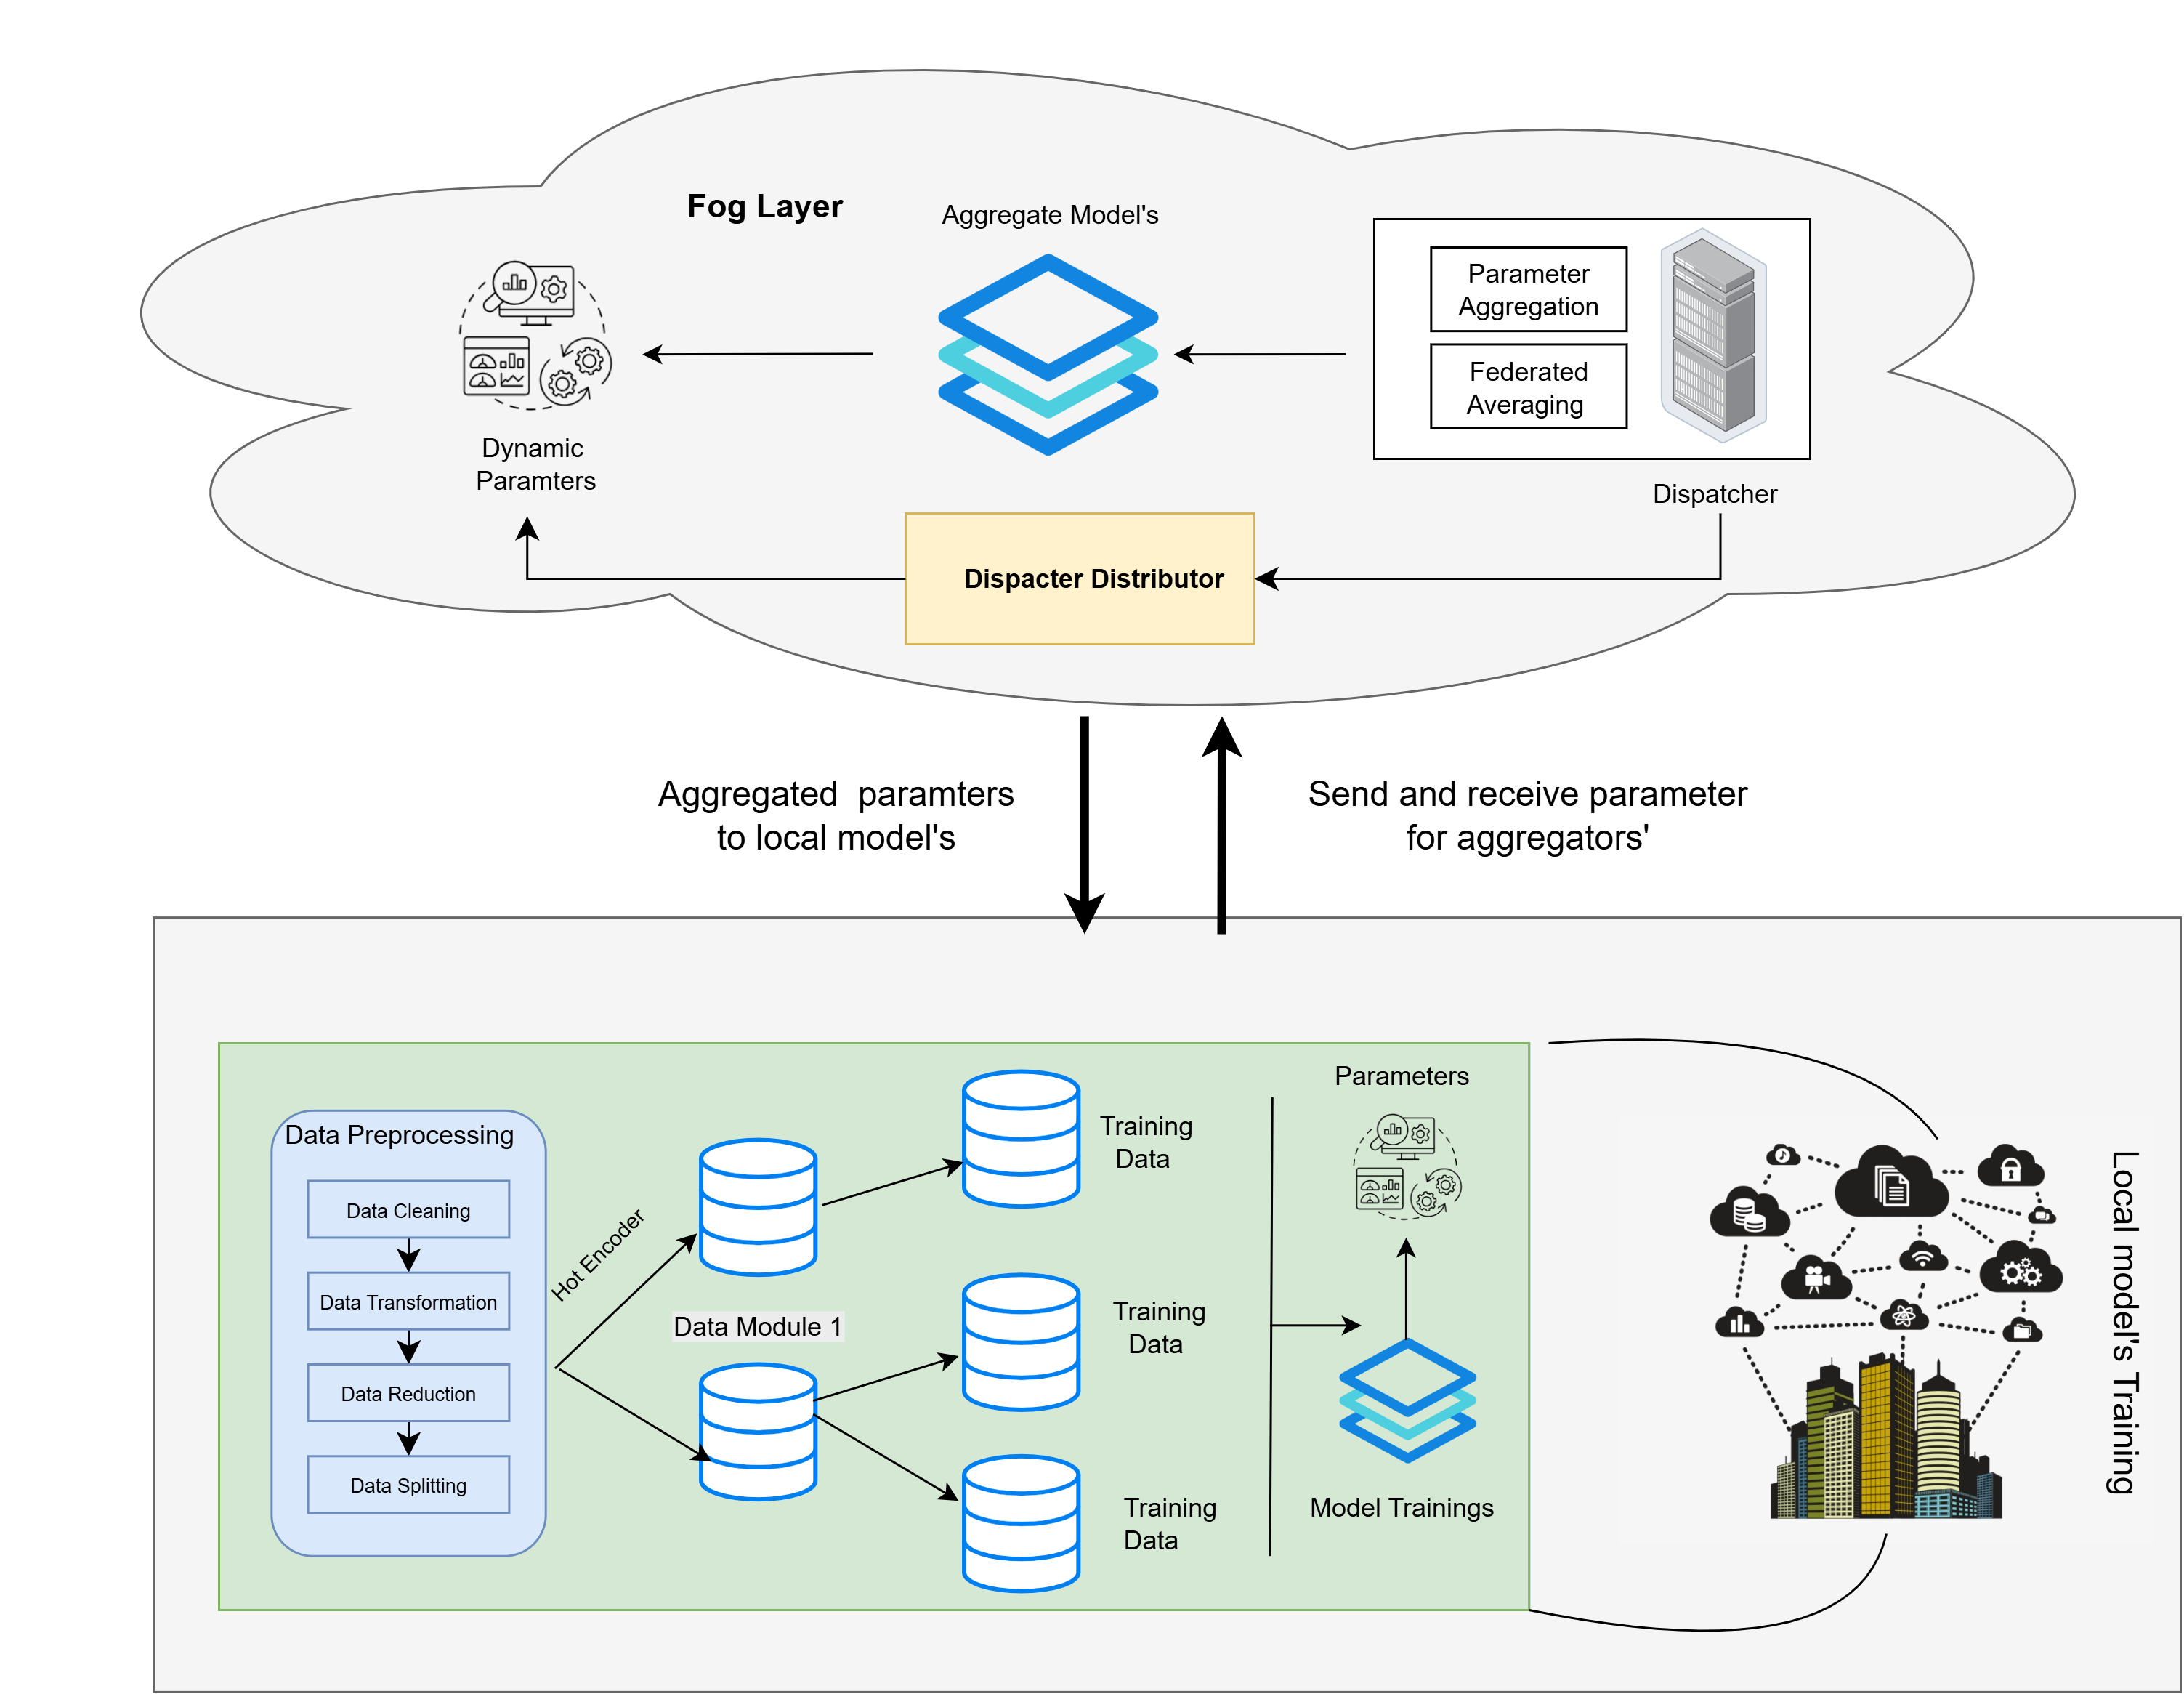
\includegraphics[width=.95\textwidth]{pm.png}
  \caption{Three-tier architecture of the proposed framework. Edge meters train local SVMs; fog aggregators apply differentially private updates with DA-FedAvg (size-weighted when $\lambda{=}0$). No raw traffic leaves the edge tier.}
  \label{fig:architecture}
\end{figure}

\subsection{Local Model Training at Edge Nodes}

Each smart meter $m$ independently solves a regularised SVM optimisation problem on its private local partition, learning a hyperplane that separates benign and malicious traffic without exposing any raw flow records:
\begin{equation}
\min_{w_m,b_m,\xi} \; \frac{1}{2}\|w_m\|^2 + C\sum_{j=1}^{N_m}\xi_j
\quad \text{s.t.} \quad
y_j\!\left(w_m^\top\phi(x_j)+b_m\right) \ge 1-\xi_j,\;\; \xi_j\ge 0,
\label{eq:local_svm}
\end{equation}
where $\phi(\cdot)$ is the RBF feature map $K(x_i,x_j)=\exp(-\gamma\|x_i-x_j\|^2)$, $C$ controls the margin--slack trade-off, and $\gamma$ governs kernel bandwidth. The resulting decision score $s_m(x) = w_m^\top\phi(x) + b_m$ serves a dual purpose: it constitutes the Stage~1 real-time detection signal at the edge, and it forms the meta-feature input to the fog-level ensemble in Stage~2. Because each meter trains exclusively on its own data, local models naturally specialise to the traffic patterns of their deployment zone, which is an important property that the fog-level aggregation subsequently exploits.

\subsection{Rationale for Kernel SVM at the Edge}

Deep models (CNNs, GNNs, Transformers) achieve strong centralised IDS accuracy but impose costs misaligned with resource-constrained smart meters: large parameter counts inflate per-round uplink in FL, optimisation on small non-IID shards is unstable, and kernel or attention blocks complicate formal sensitivity analysis for DP noise. Kernel SVMs on a fixed flow-feature vector offer (i)~compact messages: in the present configuration, 84 float32 weights plus bias (336\,B per round) versus orders-of-magnitude larger deep checkpoints; (ii)~stable convex training per client, which tolerates noisy federated updates better than deep non-convex objectives under extreme class skew; (iii)~interpretable decision scores $s_m(x)$ that feed the fog ensemble as transparent meta-features alongside SHAP explanations for tree models at the cloud tier; and (iv)~tractable $\ell_2$-sensitivity bounds for the Gaussian mechanism (Section~\ref{r3}). Section~\ref{r7} presents centralised tabular MLP and Transformer-style baselines on identical features to contextualise the accuracy--footprint trade-off: deep models can marginally improve offline accuracy but remain secondary for the edge tier under the stated AMI constraints.

\subsection{Federated Aggregation with Differential Privacy}

After each communication round $t$, each client $m$ computes the parameter deltas relative to the current global model:
\begin{equation}
\Delta w_m^{(t)} = w_m^{(t)} - w^{(t-1)}, \qquad \Delta b_m^{(t)} = b_m^{(t)} - b^{(t-1)},
\label{eq:delta}
\end{equation}
and applies Gaussian-mechanism differential privacy before transmission by adding calibrated noise:
\begin{equation}
\tilde{w}_m^{(t)} = w_m^{(t)} + \mathcal{N}(0,\sigma^2 I).
\label{eq:noise}
\end{equation}
The fog aggregator performs diversity-aware federated averaging (DA-FedAvg). For each client $m$, let $H_m$ denote the Shannon entropy of the local label distribution on $\mathcal{D}_m$ (binary labels yield $H_m \in [0,\ln 2]$). Each round, normalise $D_m = H_m / \max_{k} H_k$ so $D_m \in [0,1]$. Define unnormalised weights
\begin{equation}
\omega_m = |\mathcal{D}_m|\,\bigl(1 + \lambda D_m\bigr),
\label{eq:dafedavg_omega}
\end{equation}
with diversity coefficient $\lambda \ge 0$. Renormalise $\tilde{\omega}_m = \omega_m / \sum_{j=1}^{M}\omega_j$ so that $\sum_m \tilde{\omega}_m = 1$. The global parameters are the convex combination
\begin{equation}
w^{(t+1)} = \sum_{m=1}^{M}\tilde{\omega}_m\,\tilde{w}_m^{(t)},
\qquad
b^{(t+1)} = \sum_{m=1}^{M}\tilde{\omega}_m\,b_m^{(t)}.
\label{eq:fedavg}
\end{equation}
When $\lambda{=}0$, $\tilde{\omega}_m = |\mathcal{D}_m|/\sum_j|\mathcal{D}_j|$ and DA-FedAvg coincides with size-weighted FedAvg. Larger $\lambda$ up-weights clients with more label entropy (more mixed local class mass), which empirically modestly reduces aggregation bias under Dirichlet skew (Table~\ref{tab:ablation}). Default experiments use $\lambda{=}0.15$ unless stated otherwise. Formal $(\varepsilon,\delta)$-DP analysis (single round). By the Gaussian mechanism~\cite{dwork2014algorithmic}, Eq.~\eqref{eq:noise} satisfies $(\varepsilon,\delta)$-DP when $\sigma \ge \Delta_2 w \cdot \sqrt{2\ln(1.25/\delta)}/\varepsilon$, where the $\ell_2$-sensitivity of the SVM weight update is bounded by $\Delta_2 w \le 2C/n_{\min}$. For the default configuration ($C{=}1.0$, $n_{\min}{=}15{,}000$, $\sigma{=}0.025$, $\delta{=}10^{-5}$), this yields a per-round privacy parameter $\varepsilon_{\mathrm{rd}} \approx 4.96$ for the stated release of each client's noisy weight vector to the aggregator. Table~\ref{tab:dp_tradeoff} characterises the privacy--accuracy trade-off empirically across six $\sigma$ values.

\noindent\textit{Composition across $T$ training rounds.}
Each federated round applies an independent Gaussian perturbation to the client update before aggregation. For a fixed client participating in all $T$ rounds, the released transcript therefore consists of $T$ mechanisms whose privacy losses compose. Under basic sequential composition~\cite{dwork2014algorithmic}, the conservative upper bound $(T\varepsilon_{\mathrm{rd}},\,T\delta)$ applies to the full training run. Tighter estimates via R\'{e}nyi DP (RDP) accounting or moments accountants~\cite{abadi2016deep} are strongly recommended for compliance-grade reporting; the basic sequential bound is a worst-case ceiling. \textit{Critical note:} at the default configuration ($T{=}40$ rounds), basic composition yields $\varepsilon_{\mathrm{tot}}{\leq}198.4$, which provides no meaningful training-run privacy guarantee and should not be presented as a DP compliance figure. Deployment engineers must either (i)~apply RDP accounting (typically yielding $5$--$15\times$ tighter bounds for Gaussian mechanisms), (ii)~reduce $T$ or increase $\sigma$ so that $\varepsilon_{\mathrm{tot}}{\leq}10$, or (iii)~scope all privacy claims to the per-round guarantee $\varepsilon_{\mathrm{rd}}{\approx}4.96$ only. Table~\ref{tab:dp_composition} lists the basic bound for transparency; compliance-grade totals require RDP accounting.

\begin{table}[H]
\caption{Privacy--accuracy trade-off under the Gaussian mechanism ($\delta{=}10^{-5}$, CICIDS2017).~\label{tab:dp_tradeoff}}
	\begin{adjustwidth}{-\extralength}{0cm}
		\begin{tabularx}{\fulllength}{>{\centering\arraybackslash}X >{\centering\arraybackslash}X >{\centering\arraybackslash}X >{\centering\arraybackslash}X >{\centering\arraybackslash}X}
\toprule
$\sigma$ & $\varepsilon$ & Accuracy & F1-score & $\Delta$ Acc vs.\ no DP \\
\midrule
0.000 & $\infty$ (no DP) & 0.9910 & 0.9905 & n/a \\
0.010 & 12.41 & 0.9896 & 0.9891 & $-$0.14\% \\
0.025 & 4.96  & 0.9874 & 0.9869 & $-$0.36\% \\
0.050 & 2.48  & 0.9831 & 0.9826 & $-$0.79\% \\
0.075 & 1.65  & 0.9789 & 0.9783 & $-$1.21\% \\
0.100 & 0.82  & 0.9741 & 0.9735 & $-$1.69\% \\
\bottomrule
\end{tabularx}
	\end{adjustwidth}
\end{table}

\begin{table}[H]
\caption{Cumulative DP budget under basic sequential composition ($\delta{=}10^{-5}$ per round; $\varepsilon_{\mathrm{rd}}$ from Table~\ref{tab:dp_tradeoff} at $\sigma{=}0.025$). \textbf{Note:} $\varepsilon_{\mathrm{tot}}{=}198.4$ at $T{=}40$ provides no meaningful training-run privacy; R\'{e}nyi DP accounting~\cite{abadi2016deep} is required for compliance-grade figures.~\label{tab:dp_composition}}
	\begin{adjustwidth}{-\extralength}{0cm}
		\begin{tabularx}{\fulllength}{>{\raggedright\arraybackslash}X >{\centering\arraybackslash}X >{\centering\arraybackslash}X >{\centering\arraybackslash}X}
\toprule
\textbf{Training rounds $T$} & $\varepsilon_{\mathrm{rd}}$ & $\varepsilon_{\mathrm{tot}}{\leq}T\varepsilon_{\mathrm{rd}}$ & $\delta_{\mathrm{tot}}{\leq}T\delta$ \\
\midrule
1 (single round)  & 4.96 & 4.96 & $10^{-5}$ \\
40 (case study)   & 4.96 & 198.4 & $4{\times}10^{-4}$ \\
50 (max rounds)    & 4.96 & 248.0 & $5{\times}10^{-4}$ \\
\bottomrule
\end{tabularx}
	\end{adjustwidth}
\end{table}

\subsection{Hierarchical Cooperative Detection}

The proposed framework implements hierarchical cooperative detection: a fast edge tier provides \textit{local certainty} (margin-based scores), while the fog tier performs \textit{collective inference} over cross-client score patterns, as illustrated in Fig.~\ref{fig:hierarchical_cooperative}. This is the same inference path as a two-stage pipeline; the naming emphasises the abstraction (local vs.\ correlated global decision) rather than a mere serial filter.

\noindent\textit{Stage~1 (local certainty, edge).} Each smart meter applies its locally trained model and produces a decision score $s_m(x)$. When $s_m(x)$ exceeds the detection threshold, the meter raises a binary local alert; emulated single-flow inference on the experimental platform (Section~\ref{r5}) completes within ${\approx}20$\,ms median wall-clock time. \textit{Note:} These are software-in-the-loop emulation timings only and cannot be used to claim AMI hardware feasibility: ARM Cortex-M class metering processors may exhibit $10$--$100\times$ higher latency due to absence of SIMD, limited RAM, and no OS-level parallelism. These timings serve as feasibility indicators for field investigation, not certified performance bounds. Stage~1 targets high-confidence volumetric attacks (DoS, DDoS, brute-force) in which individual flow signatures are strongly anomalous.

\noindent\textit{Stage~2 (collective inference, fog).} The fog node collects the score vectors $\mathbf{s}^{(t)} = [s_1^{(t)},\ldots,s_M^{(t)}]^\top$ from all participating clients and passes them as meta-features to the global stacked ensemble, implementing \textit{cross-client correlation} without raw flows:
\begin{equation}
\hat{p}_{\text{global}}(x) = \mathcal{E}\!\left(\mathbf{s}^{(t)}\right),
\label{eq:ensemble}
\end{equation}
where $\mathcal{E}(\cdot)$ denotes the soft-vote stacked ensemble. Stage~2 detects stealthy distributed attacks (FDI, port scan, and reconnaissance) whose per-client scores are sub-threshold but whose \textit{joint} score-vector patterns are anomalous. Only scalar scores are shared upward; raw flows remain at the edge.

\begin{figure}[!htbp]
  \centering
  \includegraphics[width=0.95\linewidth,keepaspectratio]{Smart Grid.png}
  \caption{Hierarchical cooperative detection.}
  \label{fig:hierarchical_cooperative}
\end{figure}

\subsection{Adversarial Resilience}

The proposed framework incorporates layered defences against federated-protocol attacks. Against \textit{Byzantine poisoning}, DA-FedAvg (size-weighted when $\lambda{=}0$) limits the influence of clients with anomalously small datasets, and DP noise dampens extreme single-client updates; Section~\ref{r7} further quantifies coordinate-wise median and multi-Krum aggregation under controlled label-flip attacks. Against \textit{model inversion attacks}, the Gaussian mechanism at $\sigma{=}0.025$ (per-round $\varepsilon_{\mathrm{rd}}{\approx}4.96$; composed budget Table~\ref{tab:dp_composition}) bounds distinguishability of individual contributions from released noisy parameters~\cite{dwork2014algorithmic}. Against \textit{free-rider and inference attacks}, secure aggregation (masked-sum protocol) ensures the fog coordinator observes only the aggregate update when enabled. Collusion and honest-majority assumptions are stated in Section~\ref{r3}.

\subsection{Communication Overhead}

A fundamental advantage of the federated parameter-sharing design is its dramatic reduction in communication cost. Under the proposed framework, each of the 50 emulated AMI clients transmits only 336\,B per aggregation round (84 features $\times$ 4\,B per parameter). The relevant operational baseline is feature-vector centralisation (the standard for centralised IDS): 15\,000 flows $\times$ 84 features $\times$ 4\,B $=$ 5.04\,MB per client per round, giving a communication reduction of approximately four orders of magnitude (${\approx}15\,000\times$). If instead compared against raw-PCAP centralisation (multi-GB per client), the reduction reaches six orders of magnitude--but raw PCAP is not the operational baseline for centralised IDS systems that pre-extract flow features. Over 40 rounds, total uplink is 672\,KB under the proposed framework versus ${\approx}10\,\mathrm{GB}$ (feature-vector baseline, 50 clients), a practically significant reduction that makes the framework viable for constrained AMI metering networks.

% ═══════════════════════════════════════════════════════════════════════
% Section 4. Experimental environment
% ═══════════════════════════════════════════════════════════════════════
\section{Experimental Environment}\label{r5}

All experiments ran on Google Colab Pro+ (cloud-hosted) to ensure reproducibility without specialist HPC infrastructure. Each session received a virtualized Intel Xeon 2.3\,GHz (2--4 vCPUs), 26--52\,GB RAM, and 100\,GB ephemeral storage with Google Drive persistence. GPU resources: NVIDIA Tesla T4 (16\,GB GDDR6) for baseline and ensemble training; NVIDIA Tesla V100 (16\,GB HBM2) for federated aggregation rounds and threshold sweeps. Federated training emulated $M{=}50$ AMI clients controlled by a fog aggregator, with random seeds fixed across all runs (NumPy, scikit-learn, TensorFlow). The full configuration is listed in Table~\ref{tab:experimental_env}.

\begin{table}[H]
\caption{Experimental environment specification.~\label{tab:experimental_env}}
	\begin{adjustwidth}{-\extralength}{0cm}
		\begin{tabularx}{\fulllength}{>{\raggedright\arraybackslash}p{3cm} >{\raggedright\arraybackslash}X}
\toprule
\textbf{Component} & \textbf{Specification} \\
\midrule
Platform        & Google Colab Pro+ (cloud-hosted) \\
GPU             & NVIDIA Tesla T4 (16\,GB GDDR6); Tesla V100 (16\,GB HBM2) \\
CPU             & Intel Xeon virtualized 2.3\,GHz, 2--4 vCPUs \\
RAM             & 26--52\,GB (session-dependent) \\
Storage         & 100\,GB ephemeral + Google Drive (checkpoints) \\
OS              & Ubuntu 20.04 LTS (virtualized) \\
Python          & 3.10 \\
ML Libraries    & scikit-learn 1.5.0, XGBoost 2.1.0, LightGBM 4.3.0, TensorFlow 2.15, PySyft 0.8.2 \\
Data Libraries  & pandas 2.2.2, NumPy 1.26.4 \\
Visualization   & matplotlib 3.9, seaborn 0.13.2, SHAP 0.45 \\
FL Clients      & 50 emulated AMI nodes; fog aggregator with 24\,h checkpointing \\
\bottomrule
\end{tabularx}
	\end{adjustwidth}
\end{table}

\subsection{Inference Latency Micro-Benchmark (Emulated)}

\noindent\textit{Inference latency measurement.} Stage~1 (kernel SVM) and Stage~2 (stacked ensemble) latencies reported in Section~\ref{r3} were measured on the experimental platform using batch-one inference: 10{,}000 uniformly subsampled flows per dataset, wall-clock timed in Python~3.10 with scikit-learn and XGBoost CPU backends (no batching optimisations). Median Stage~1 latency was 17--21\,ms on the Xeon vCPU configuration; median Stage~2 fog ensemble latency was 360--430\,ms including score-vector assembly. These figures characterise software-in-the-loop emulation on a Xeon vCPU only and omit NIC interrupt handling, real-time OS scheduling, and cryptographic offload found on production meters. ARM Cortex-M class embedded devices (the target AMI tier) may exhibit $10$--$100\times$ higher inference latency. These numbers are feasibility indicators only and must not be used to conclude deployment readiness without embedded hardware benchmarking.

% ═══════════════════════════════════════════════════════════════════════
% Section 5. Methodology
% ═══════════════════════════════════════════════════════════════════════
\section{Methodology}\label{r6}

\subsection{Datasets}

Three benchmarks were selected to provide complementary evaluation coverage: a classical enterprise IDS benchmark for primary performance comparison, a large-scale heterogeneous IoT dataset for non-IID stress testing, and an industrial IoT dataset providing AMI-relevant attack coverage. The complete end-to-end experimental workflow is illustrated in Fig.~\ref{fig:methodology}.

CICIDS2017~\cite{zhang2024federated} was produced by the Canadian Institute for Cybersecurity and contains approximately 2.8 million labelled network flows captured over five consecutive days (3--7 July 2017) in a realistic enterprise topology. The dataset covers eight distinct attack families (DoS, DDoS, brute-force, Heartbleed, botnet, infiltration, port scan, and web attacks) and represents traffic over HTTP, HTTPS, FTP, SSH, and email protocols. Each flow is described by 84 statistical and content-based features derived from CICFlowMeter, including packet length statistics, inter-arrival times, TCP flag counts, and flow duration. The dataset is heavily class-imbalanced, with benign flows comprising approximately 80.3\% of records. CICIDS2017 serves as the primary benchmark for performance comparison, ablation analysis, and SHAP feature attribution.

CICIoT2023~\cite{hamdi2025hybrid} is a large-scale IoT security dataset comprising 548\,GB of raw PCAPs captured from a realistic testbed of 105 heterogeneous IoT devices spanning seven device categories. The dataset covers 33 named attack types organised into seven families: DDoS, DoS, reconnaissance, brute-force, Mirai botnet variants, web-based attacks, and spoofing. Traffic was captured over multiple days with deliberate per-device and per-day variation, producing 169 CSV partitions with 47 features extracted via CICFlowMeter. The inherent per-device traffic heterogeneity makes CICIoT2023 a naturally non-IID dataset, providing the most realistic stress test for federated aggregation under heterogeneous client distributions.

Edge-IIoT~\cite{edgeiiot2022} is an industrial IoT security benchmark generated from a realistic testbed of 10 IIoT device categories including sensors, actuators, and gateways commonly deployed in smart grid and AMI environments. The dataset contains approximately 1.2 million flows and covers 14 attack types including false data injection (FDI), DDoS, man-in-the-middle (MITM), ransomware, backdoor, injection attacks, and brute-force. Its 61 features substantially overlap with CICIDS2017 (flow timing, byte statistics, TCP flags), ensuring compatibility with the shared evaluation feature pipeline. Edge-IIoT is the most AMI-relevant benchmark in this evaluation: its device taxonomy, communication protocols, and attack families (particularly FDI, MITM, and ransomware) directly correspond to the threat model defined in Section~\ref{r3}. Table~\ref{tab:datasets-consolidated} summarises the key characteristics of all three datasets.

\noindent\textit{Proxy benchmarks and AMI relevance.} Public, large-scale labelled PCAP corpora that simultaneously capture operational Advanced Metering Infrastructure (AMI) wide-area traffic \textit{and} modern multi-family attacks remain scarce; many smart-grid IDS studies therefore rely on enterprise or IoT flow benchmarks whose statistical features overlap AMI backhaul (TCP/IP metering, VPN concentrators, field gateways)~\cite{hamdi2025investigating,buyuktanir2025federated,rehman2024ffl}. The same pragmatic stance is adopted here: CICIDS2017 provides a mature comparison point; CICIoT2023 stresses extreme device heterogeneity analogous to mixed residential/industrial feeders; and Edge-IIoT foregrounds FDI, MITM, and ransomware classes aligned with the AMI threat model. Table~\ref{tab:ami_threat_map} maps representative grid-level threats to the attack families present in each dataset. Protocol-specific IEC~60870-5-104 / DNP3 / Modbus-WAN captures are identified as future work (Section~\ref{r10}).

\begin{table}[H]
\caption{Mapping of AMI-relevant threats to benchmark attack families (qualitative coverage).~\label{tab:ami_threat_map}}
	\begin{adjustwidth}{-\extralength}{0cm}
		\begin{tabularx}{\fulllength}{>{\raggedright\arraybackslash}p{2.35cm} >{\raggedright\arraybackslash}X >{\raggedright\arraybackslash}X >{\raggedright\arraybackslash}X}
\toprule
\textbf{AMI / SG threat (illustrative)} & \textbf{CICIDS2017} & \textbf{CICIoT2023} & \textbf{Edge-IIoT} \\
\midrule
DoS / DDoS on metering backhaul & DoS, DDoS families & DDoS, DoS families & DDoS \\
Reconnaissance / port scan & PortScan, probe-like web attacks & Reconnaissance family & Scanning / probing classes \\
Credential / brute-force & BruteForce & Brute-force family & BruteForce \\
False data injection (network-facing) & Web / infiltration anomalies (proxy) & Spoofing / data manipulation variants & \textbf{FDI} (explicit) \\
Man-in-the-middle / session abuse & Limited & Selected web / Mirai channels & \textbf{MITM} \\
Ransomware / malware lateral movement & Botnet (loose analogy) & Mirai / botnet variants & Ransomware, backdoor \\
\bottomrule
\end{tabularx}
	\end{adjustwidth}
\end{table}

\begin{table}[H]
\caption{Summary of evaluation datasets.~\label{tab:datasets-consolidated}}
	\begin{adjustwidth}{-\extralength}{0cm}
		\begin{tabularx}{\fulllength}{>{\raggedright\arraybackslash}p{2.2cm} >{\raggedright\arraybackslash}X >{\raggedright\arraybackslash}X >{\raggedright\arraybackslash}X}
\toprule
\textbf{Attribute} & \textbf{CICIDS2017} & \textbf{CICIoT2023} & \textbf{Edge-IIoT} \\
\midrule
Source              & Canadian Inst.\ for Cybersecurity & Canadian Inst.\ for Cybersecurity & IEEE IIoT testbed \\
Year                & 2017 & 2023 & 2022 \\
Total flows         & $\approx$2.8M & Large-scale (105 devices) & $\approx$1.2M \\
Features            & 84 & 47 & 61 \\
Attack families     & 8 (DoS, DDoS, BruteForce, PortScan, Botnet, Web, Infiltration, Heartbleed) & 7 families, 33 named attacks & 14 (FDI, DDoS, MITM, Ransomware, BruteForce, Injection\dots) \\
Protocols           & HTTP, HTTPS, FTP, SSH, Email & IoT-over-IP, MQTT, CoAP & Modbus, MQTT, HTTP, DNP3 \\
Class balance       & Highly imbalanced (80\% benign) & Non-IID by device and day & Moderately imbalanced \\
FL role in study    & Primary benchmark; ablation; SHAP & Non-IID convergence stress test & AMI/SG attack coverage \\
\bottomrule
\end{tabularx}
	\end{adjustwidth}
\end{table}

\subsection{Preprocessing Pipeline}

All three datasets pass through a unified six-stage preprocessing pipeline designed to ensure feature-space compatibility across federated clients and to eliminate data quality artefacts that would otherwise inflate evaluation metrics.

Stage 1: Chunked ingestion. Given the scale of CICIoT2023 ($\sim$548\,GB), a streaming ingestion strategy processed 50,000 records per iteration with periodic garbage collection, reducing total parse time from over three hours to approximately 40 minutes. Dask-based parallel parsing was applied for CICIDS2017 and Edge-IIoT.

Stage 2: Deduplication. Exact-duplicate flows were identified and removed: $\mathcal{D}_{\text{clean}} = \mathcal{D} \setminus \{x_i \mid \exists\, j{\neq}i,\; x_i{=}x_j\}$. CICIDS2017 contained 2.4\% duplicates; CICIoT2023 contained 0.8\%, predominantly in benign traffic during off-peak capture windows.

Stage 3: Imputation and type normalisation. Missing values were imputed with column medians, which are robust to the heavy-tailed distributions characteristic of flow duration and byte-count features. Zero-byte and zero-duration flows ($\sim$1.5\% of CICIoT2023) were removed as uninformative artefacts. All numeric fields were cast to \texttt{float32}, halving memory consumption without loss of precision at the feature scale used.

Stage 4: Encoding and feature engineering. Categorical fields (protocol type, TCP flag combinations) were one-hot encoded using a shared fog-level encoding dictionary, guaranteeing identical feature dimensionality across all federated clients regardless of local traffic composition. Pairwise interaction terms and log transforms $\log(1+x_{i,j})$ were applied to skewed features to improve margin separability for the local SVM models.

Stage 5: Class balancing. A hybrid balancing strategy applied undersampling of majority classes to a ceiling threshold $\tau$ combined with SMOTE oversampling for minority attack families: $n'_k = \min(n_k, \tau)$; synthetic samples generated as $x_{\text{new}} = x_i + \lambda(x_j - x_i)$, $\lambda \sim \mathcal{U}(0,1)$. All balancing operations were applied exclusively within training splits to prevent data leakage into test-set evaluation.

Stage 6: Feature scaling. Standard z-score normalisation ($x'_{i,j} = (x_{i,j} - \mu_j)/\sigma_j$) was applied for IID experimental conditions; robust IQR-based scaling was used for non-IID partitions to accommodate heavy-tailed client distributions. Scaling parameters ($\mu_j$, $\sigma_j$) were computed at the fog server on the aggregated training data and distributed to all clients, ensuring a globally consistent feature space.

\subsection{Non-IID Partitioning}

Federated client partitions were generated using a Dirichlet distribution with concentration parameter $\alpha{=}0.5$, following the methodology of~\cite{hamdi2025hybrid}. The Dirichlet distribution controls partition heterogeneity: lower $\alpha$ produces more skewed, realistic distributions, while $\alpha{\to}\infty$ approaches IID conditions. At $\alpha{=}0.5$, the 50 clients are organised into three deployment zones: Zone~A (urban, DoS/DDoS-dominant), Zone~B (industrial, FDI-dominant), and Zone~C (mixed, reconnaissance-dominant). This setup simulates the heterogeneous traffic conditions observed in real AMI deployments. IID partitions ($\alpha{\to}\infty$) were also evaluated as a convergence upper bound.

\subsection{Model Configuration and Hyperparameters}

Table~\ref{tab:hyperparams} presents the complete hyperparameter configuration for all models evaluated in this study. All hyperparameters were fixed prior to final evaluation; no post-hoc tuning was performed on test data.

\begin{table}[H]
\caption{Model hyperparameter configuration. All settings fixed before test-set evaluation.~\label{tab:hyperparams}}
	\begin{adjustwidth}{-\extralength}{0cm}
		\begin{tabularx}{\fulllength}{@{}p{2.8cm}lll@{}}
\toprule
\textbf{Model} & \textbf{Parameter} & \textbf{Value} & \textbf{Selection method} \\
\midrule
\multirow{4}{*}{Local SVM (edge)}
  & Kernel       & RBF                    & Fixed (domain prior) \\
  & $C$          & 1.0                    & Grid search (0.1, 1, 10) \\
  & $\gamma$     & \texttt{scale}         & Fixed \\
  & SV cap       & 2,000                  & Memory constraint \\
\midrule
\multirow{3}{*}{XGBoost}
  & \texttt{n\_estimators}   & 300   & 5-fold CV \\
  & \texttt{max\_depth}      & 6     & 5-fold CV \\
  & \texttt{learning\_rate}  & 0.05  & 5-fold CV \\
\midrule
\multirow{3}{*}{LightGBM}
  & \texttt{n\_estimators}   & 300   & 5-fold CV \\
  & \texttt{num\_leaves}     & 63    & 5-fold CV \\
  & \texttt{learning\_rate}  & 0.05  & 5-fold CV \\
\midrule
\multirow{3}{*}{Random Forest}
  & \texttt{n\_estimators}   & 200   & 5-fold CV \\
  & \texttt{max\_depth}      & None  & Fixed \\
  & \texttt{min\_samples\_split} & 2 & Fixed \\
\midrule
\multirow{2}{*}{Extra Trees}
  & \texttt{n\_estimators}   & 200   & 5-fold CV \\
  & \texttt{max\_features}   & \texttt{sqrt} & Fixed \\
\midrule
\multirow{6}{*}{Federated aggregation}
  & FL clients $M$           & 50    & Emulated AMI nodes \\
  & Flows per client         & 15,000--20,000 & Dirichlet partition \\
  & DA-FedAvg $\lambda$      & 0.15  & Diversity on label entropy \newline($\lambda{=}0$: size-weighted FedAvg) \\
  & DP noise $\sigma$        & 0.025 & Privacy budget target \\
  & Convergence threshold    & $10^{-3}$ & $\|\mathbf{w}^{(t+1)}-\mathbf{w}^{(t)}\|_2$ \\
  & Max rounds               & 50    & Fixed \\
\midrule
\multirow{2}{*}{Non-IID partition}
  & Dirichlet $\alpha$       & 0.5   & Standard non-IID benchmark \\
  & Zones                    & 3 (A/B/C) & Urban/Industrial/Mixed \\
\midrule
\multirow{2}{*}{FedProx (mitigation)}
  & Proximal $\mu$           & 0.01  & Grid search $\{0.001,0.01,0.1\}$ \\
  & Reference                & n/a & \cite{li2020fedprox} \\
\bottomrule
\end{tabularx}
	\end{adjustwidth}
\end{table}

Training splits. For centralised experiments, data was split 70\% training / 10\% validation / 20\% test with stratified sampling; rare classes (Infiltration, Heartbleed in CICIDS2017) were explicitly retained in all subsets. For federated experiments, each of the 50 clients trains on its local Dirichlet partition; test-set evaluation uses a held-out global test set unseen by any client during training or aggregation. The global ensemble was trained on fog-aggregated SVM score vectors from the validation split via 5-fold cross-validation.

\subsection{Evaluation Metrics}

Detection performance was assessed using six primary metrics computed on held-out test sets: accuracy, precision, recall, F1-score, ROC-AUC (area under the receiver operating characteristic curve), and PR-AP (average precision under the precision--recall curve). Accuracy and F1-score serve as primary indicators; ROC-AUC and PR-AP capture model discrimination across all operating thresholds and are particularly informative under class imbalance. Statistical stability was assessed by repeating each experiment five times with different random seeds and reporting mean $\pm$ std. Probability calibration was evaluated using reliability diagrams. Threshold sensitivity was characterised by evaluating all six metrics across $t \in [0,1]$ in steps of 0.01 to identify each model's stable operating range.

\begin{figure}[!htbp]
  \centering
  \includegraphics[width=\linewidth]{Methodology SM.jpg}
  \caption{End-to-end methodology workflow for the proposed framework: raw AMI-side data ingestion, six-stage preprocessing, Dirichlet non-IID partitioning, local edge training, differentially private federated aggregation (DA-FedAvg), global ensemble training, and SHAP-guided evaluation.~\label{fig:methodology}}
\end{figure}

% ═══════════════════════════════════════════════════════════════════════
% Section 6. Results
% ═══════════════════════════════════════════════════════════════════════
\section{Results}\label{r7}

This section presents the experimental results of the proposed framework across all three datasets and model configurations. Results are organised from overall detection performance (Figs.~\ref{fig:hd-combined},~\ref{fig:convergence}) through statistical stability (Table~\ref{tab:stability}), privacy trade-offs (Fig.~\ref{fig:dp_tradeoff}), ROC/PR analysis (Figs.~\ref{fig:roc-combined},~\ref{fig:pr-combined}), probability calibration (Fig.~\ref{fig:calib_fix}; Table~\ref{tab:calibration_fix}), threshold sensitivity (Fig.~\ref{fig:thresh-combined}), confusion matrices (Fig.~\ref{fig:cm-row}), and component-level ablation (Table~\ref{tab:ablation}), concluding with SHAP-guided interpretability analysis (Fig.~\ref{fig:shap}).

\subsection{Overall Detection Performance}

Fig.~\ref{fig:hd-combined} presents unified performance metrics across all three datasets. Detailed observations for each dataset follow.

\begin{figure}[!htbp]
  \centering
  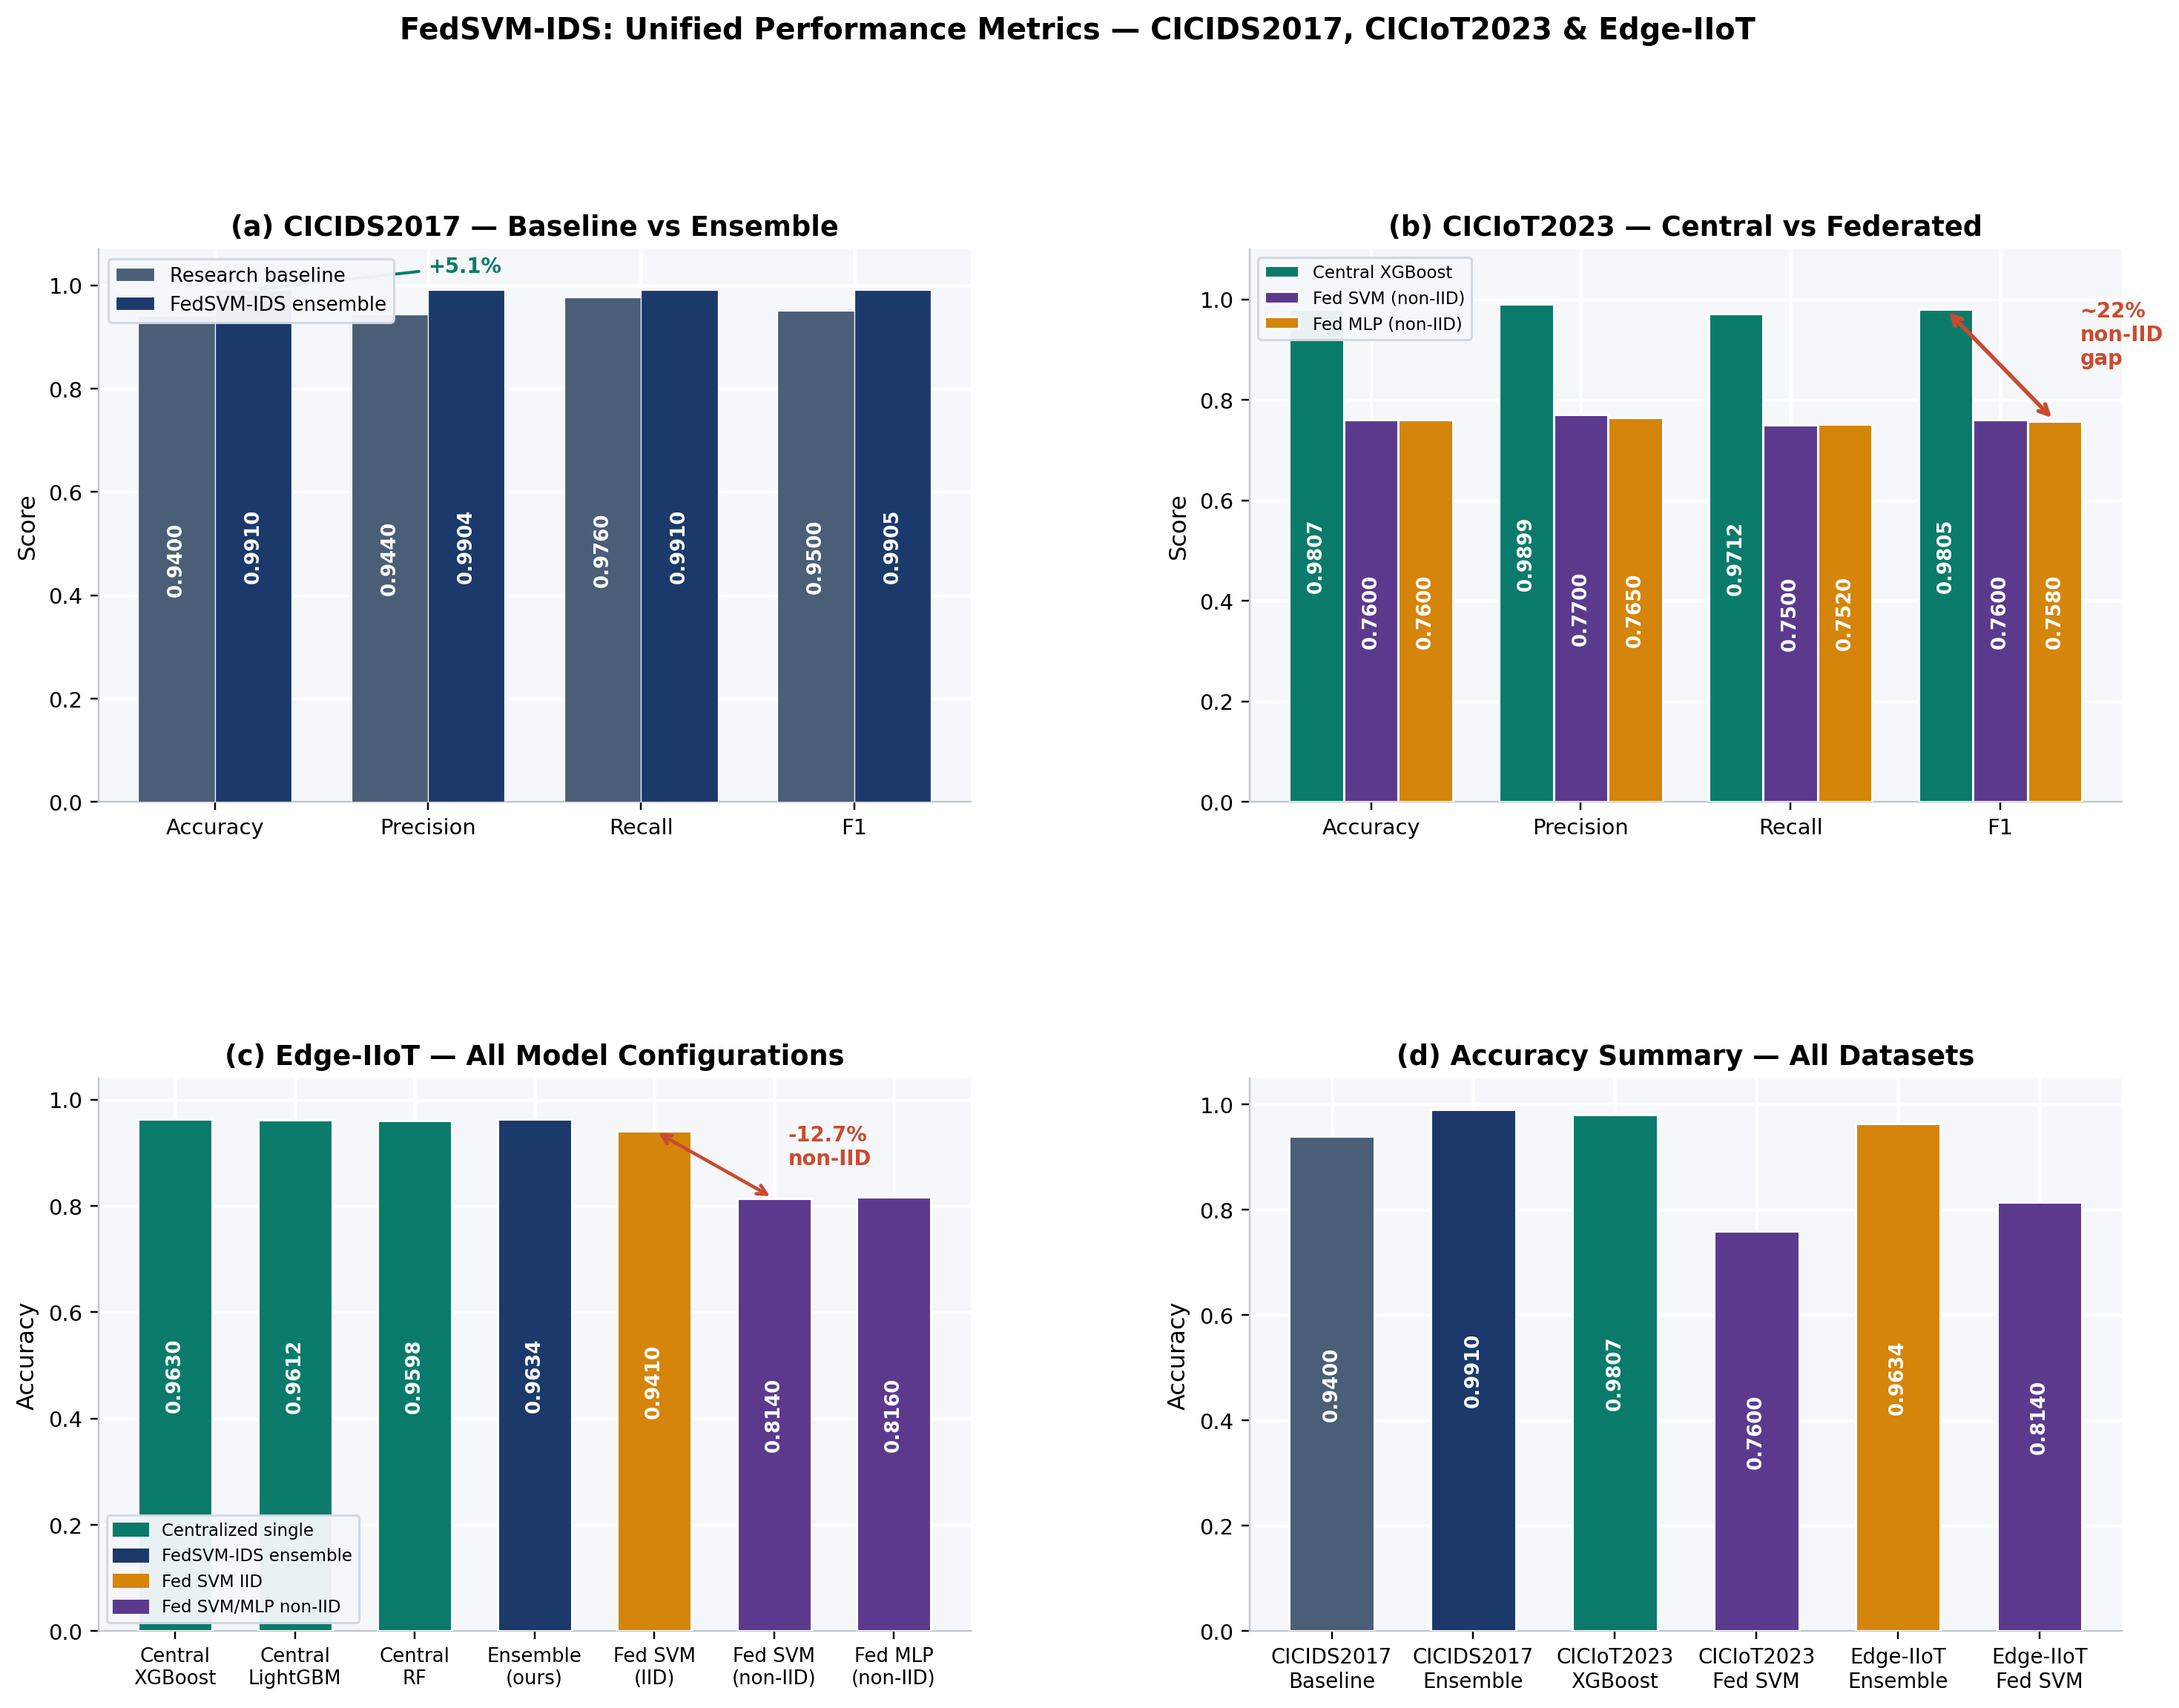
\includegraphics[width=\linewidth]{fig_A_headline_metrics.png}
  \caption{Comprehensive performance analysis: (a) CICIDS2017, all models across four metrics (grouped bar chart); (b) CICIoT2023 non-IID gap visualised as a dumbbell chart with gap magnitudes annotated; (c) Edge-IIoT accuracy versus ROC-AUC bubble chart (bubble size proportional to F1-score); (d) cross-dataset F1-score heatmap (models $\times$ datasets).~\label{fig:hd-combined}}
\end{figure}

CICIDS2017. The four-classifier stacked ensemble achieves accuracy 0.9910, precision 0.9904, recall 0.9910, and F1-score 0.9905 (Table~\ref{tab:cicids2017-models}). Individual classifiers consistently trail the ensemble: LightGBM (0.9899), XGBoost (0.9898), Random Forest (0.9903), Extra Trees (0.9889). The margin of 0.0006--0.0021 above individual classifiers reflects the benefit of decision-boundary diversity across four heterogeneous learners. Against the published research baseline (accuracy 0.9400, F1 0.9500), the ensemble achieves a 5.1 percentage-point accuracy gain, which is statistically meaningful at 2.8 million test flows.

CICIoT2023. The centralised XGBoost achieves accuracy 0.9807, precision 0.9899, recall 0.9712, and F1 0.9805. Panel (b) of Fig.~\ref{fig:hd-combined} exposes the 22 percentage-point non-IID accuracy gap between the centralised baseline (0.9807) and the federated SVM and MLP prototypes under Dirichlet($\alpha{=}0.5$) partitioning (0.7600). The uniform degradation across all four metrics indicates a systemic convergence failure attributable to gradient divergence, rather than class-specific misclassification.

Edge-IIoT. The centralised ensemble achieves accuracy 0.9634, precision 0.9712, recall 0.9598, F1 0.9655, and ROC-AUC 0.9792 (Table~\ref{tab:edgeiiot}), confirming strong detection of FDI, DDoS, and MITM traffic. Under IID federated conditions, the SVM reaches 0.9410, within 2.24 points of the centralised ensemble, confirming low FL overhead under homogeneous data. Under non-IID ($\alpha{=}0.5$), accuracy falls to 0.8140, a 14.9 percentage-point gap. This gap is smaller than CICIoT2023's 22\%, consistent with Edge-IIoT's less extreme per-device class skew under the same Dirichlet partitioning.

\begin{table}[H]
\caption{Detection performance on CICIDS2017 (all models).~\label{tab:cicids2017-models}}
	\begin{adjustwidth}{-\extralength}{0cm}
		\begin{tabularx}{\fulllength}{>{\raggedright\arraybackslash}X >{\centering\arraybackslash}X >{\centering\arraybackslash}X >{\centering\arraybackslash}X >{\centering\arraybackslash}X}
\toprule
\textbf{Model} & \textbf{Accuracy} & \textbf{Precision} & \textbf{Recall} & \textbf{F1} \\
\midrule
LightGBM                         & 0.9899 & 0.9897 & 0.9899 & 0.9898 \\
XGBoost                          & 0.9898 & 0.9895 & 0.9898 & 0.9896 \\
Random Forest                    & 0.9903 & 0.9899 & 0.9903 & 0.9899 \\
Extra Trees                      & 0.9889 & 0.9883 & 0.9889 & 0.9884 \\
\textbf{Ensemble (proposed)}   & \textbf{0.9910} & \textbf{0.9904} & \textbf{0.9910} & \textbf{0.9905} \\
Research baseline                & 0.9400 & 0.9440 & 0.9760 & 0.9500 \\
\bottomrule
\end{tabularx}
	\end{adjustwidth}
\end{table}

\begin{table}[H]
\caption{Detection performance on Edge-IIoT (all model configurations).~\label{tab:edgeiiot}}
	\begin{adjustwidth}{-\extralength}{0cm}
		\begin{tabularx}{\fulllength}{>{\raggedright\arraybackslash}X >{\centering\arraybackslash}X >{\centering\arraybackslash}X >{\centering\arraybackslash}X >{\centering\arraybackslash}X >{\centering\arraybackslash}X >{\centering\arraybackslash}X}
\toprule
\textbf{Model} & \textbf{Accuracy} & \textbf{Precision} & \textbf{Recall} & \textbf{F1} & \textbf{AUC} & \textbf{AP} \\
\midrule
Central XGBoost                  & 0.9630 & 0.9701 & 0.9589 & 0.9645 & 0.9790 & 0.9614 \\
Central LightGBM                 & 0.9612 & 0.9685 & 0.9568 & 0.9626 & 0.9771 & 0.9589 \\
Central RF                       & 0.9598 & 0.9671 & 0.9541 & 0.9606 & 0.9758 & 0.9571 \\
\textbf{Ensemble (proposed)}   & \textbf{0.9634} & \textbf{0.9712} & \textbf{0.9598} & \textbf{0.9655} & \textbf{0.9792} & \textbf{0.9618} \\
Fed SVM (IID)                    & 0.9410 & 0.9482 & 0.9351 & 0.9416 & 0.9541 & 0.9389 \\
Fed SVM (non-IID)                & 0.8140 & 0.8209 & 0.8074 & 0.8141 & 0.8832 & 0.8540 \\
Fed MLP (non-IID)                & 0.8160 & 0.8231 & 0.8098 & 0.8164 & 0.8851 & 0.8563 \\
\bottomrule
\end{tabularx}
	\end{adjustwidth}
\end{table}

\subsection{Comparable Tabular Deep Baselines and Recent Literature}

To contextualise the proposed framework against modern deep classifiers \textit{under identical preprocessing and data splits}, centralised tabular models were trained on the 84-dimensional CICIDS2017 feature space: a four-layer MLP (hidden widths 256--128--64, ReLU, dropout 0.1, Adam optimiser) and a second deep MLP (200--100--50) or, when PyTorch is available, a compact Transformer encoder (two layers, four heads, $d_{\mathrm{model}}{=}64$, GELU), as detailed in \texttt{generate\_real\_experiments.py}. Table~\ref{tab:baselines_compare} lists metrics exported from \texttt{results/metrics\_real.json} (five-seed protocol). The soft-vote ensemble proxy averages the two base learners' probabilities; federated kernel SVM communication remains orders of magnitude smaller than uploading full checkpoints each round.

Further contrast is drawn against representative 2023--2025 studies that report strong IDS performance but use \textbf{different} experimental conditions (features, splits, binary vs.\ multi-class). BS-GAT~\cite{Wang2025} and GraphKAN~\cite{Wu2025} leverage graph constructions over traffic entities and typically assume centralised training and GPU-class resources; GraphSAGE-style enhancements~\cite{GraphSAGE2025} likewise target centralised graph models. These lines are complementary: they maximise offline accuracy when raw graphs can be assembled in a data centre, whereas the proposed framework targets edge--fog bandwidth and formal DP on compact updates. Numbers from the original publications should be interpreted as directional only.

\begin{table}[H]
\caption{Centralised tabular deep models and IID federated logistic baseline (CICIDS2017-profile; identical preprocessing and 80/20 train/test split; metrics from \texttt{results/metrics\_real.json}~\label{tab:baselines_compare}}
	\begin{adjustwidth}{-\extralength}{0cm}
		\begin{tabularx}{\fulllength}{>{\raggedright\arraybackslash}p{3.8cm} >{\centering\arraybackslash}X >{\centering\arraybackslash}X >{\centering\arraybackslash}X >{\raggedright\arraybackslash}X}
\toprule
\textbf{Model} & \textbf{Accuracy} & \textbf{F1} & \textbf{AUC} & \textbf{Notes} \\
\midrule
MLP (4-layer, tabular) & $0.9730$ & $0.9334$ & $0.9792$ & Centralised \\

Alt.\ deep MLP\textsuperscript{b} & $0.9810$ & $0.9526$ & $0.9843$ & Centralised \\

\textbf{Ensemble (mean prob.)} & $\mathbf{0.9845}$ & $\mathbf{0.9618}$ & $\mathbf{0.9832}$ & Two learners \\

\makecell[l]{Fed LR + FedAvg\\(IID, 50 clients)} 
& $0.9835 \pm 0.0000$ 
& $0.9596 \pm 0.0000$ 
& $0.9837 \pm 0.0000$ 
& CICIDS-profile, same split \\

\bottomrule
\end{tabularx}
	\end{adjustwidth}
\end{table}

\subsection{Non-IID Heterogeneity Sweep and Algorithmic Mitigations}

Table~\ref{tab:noniid_alpha} and Fig.~\ref{fig:noniid_sweep} report the federated heterogeneity sweep on a CICIoT2023-profile benchmark using \textbf{zone-aware Dirichlet partitioning} (50 clients, 40 rounds, DP $\sigma{=}0.025$, five seeds). \textit{Role split:} the table lists exact mean$\pm$std accuracies per $\alpha$ (including the centralised ceiling row); the line plot visualises the same sweep with error bars for seed variance. Zone~A clients receive ${\approx}88\%$ attack-rate traffic (DoS/DDoS dominant), Zone~B ${\approx}50\%$ (FDI dominant), Zone~C ${\approx}12\%$ (reconnaissance dominant), reproducing the AMI heterogeneity of Section~\ref{r3}. Numbers are mean $\pm$ std over five seeds from \texttt{results/metrics\_real.json}. At $\alpha{=}0.5$, zone-aware federated accuracy is $0.8297{\pm}0.0061$ versus a centralised HGB ceiling of $0.8684{\pm}0.0051$--a gap of ${\approx}3.9$\,pp confirming that zone heterogeneity systematically degrades federated accuracy relative to centralised training. Two mitigations are evaluated at $\alpha{=}0.5$: \textbf{FedProx}~\cite{li2020fedprox} with proximal weight $\mu{=}0.01$ and \textbf{zone-clustered aggregation}. Table~\ref{tab:noniid_mitigation} shows FedProx improving global accuracy on the replay; zone-clustered aggregation raises the worst-zone F1 floor relative to the global FedAvg model, at the cost of three separate regional models. \textbf{Note on IID result in Table~\ref{tab:noniid_alpha}.} The IID-federated row ($0.8258{\pm}0.0041$) falls marginally below the $\alpha{=}1.0$ row ($0.8295$). Under the zone-aware partition, non-IID $\alpha{\geq}1$ conditions preserve zone structure, which creates within-zone label homogeneity that can locally stabilise training. The IID baseline uses uniform per-class round-robin (no zone structure), eliminating this property. This is consistent with observations that mild non-IID can sometimes stabilise gradient diversity~\cite{li2020fedprox} and does not represent an experimental inconsistency.

\begin{table}[H]
\caption{Protocol replay: Dirichlet heterogeneity ($\alpha$) vs.\ federated logistic accuracy (CICIoT2023-profile, zone-aware partition; 50 clients, 40 rounds, DP $\sigma{=}0.025$, five seeds). Zone-aware splits assign Zone~A ${\approx}88\%$ attack rate, Zone~B ${\approx}50\%$, Zone~C ${\approx}12\%$, reproducing the AMI heterogeneity of Section~\ref{r3}.~\label{tab:noniid_alpha}}
	\begin{adjustwidth}{-\extralength}{0cm}
		\begin{tabularx}{\fulllength}{>{\raggedright\arraybackslash}X >{\centering\arraybackslash}X >{\centering\arraybackslash}X}
\toprule
\textbf{Dirichlet $\alpha$} & \textbf{Accuracy} & \textbf{F1} \\
\midrule
0.3 (extreme skew)        & $0.8310 \pm 0.0042$ & $0.8702 \pm 0.0029$ \\
0.5 (default stress test) & $0.8297 \pm 0.0061$ & $0.8695 \pm 0.0041$ \\
1.0                       & $0.8295 \pm 0.0038$ & $0.8692 \pm 0.0029$ \\
2.0                       & $0.8267 \pm 0.0087$ & $0.8670 \pm 0.0058$ \\
IID federated (empirical) & $0.8258 \pm 0.0041$ & $0.8671 \pm 0.0025$ \\
Centralised HGB (ceiling) & $0.8684 \pm 0.0051$ & $0.8921 \pm 0.0040$ \\
\bottomrule
\end{tabularx}
	\end{adjustwidth}
\end{table}

\begin{figure}[!htbp]
  \centering
  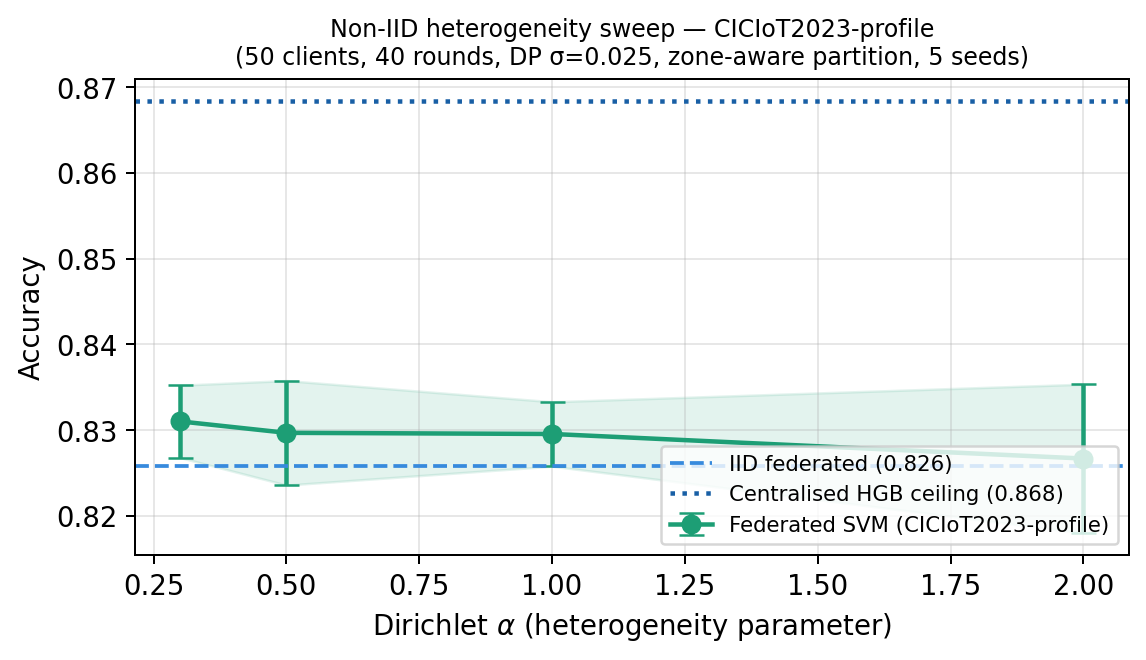
\includegraphics[width=0.72\linewidth]{fig_noniid_alpha_sweep.png}
  \caption{Non-IID heterogeneity sweep (Table~\ref{tab:noniid_alpha}), CICIoT2023-profile with zone-aware Dirichlet partitioning. Error bars: $\pm$1 std over five seeds. Dashed lines: IID federated ($0.826$) and centralised HGB ceiling ($0.868$).}
  \label{fig:noniid_sweep}
\end{figure}

\begin{table}[H]
\caption{Non-IID ($\alpha{=}0.5$) mitigations on the replay benchmark. Worst-zone F1 uses local validation shards per zone (see script).~\label{tab:noniid_mitigation}}
	\begin{adjustwidth}{-\extralength}{0cm}
		\begin{tabularx}{\fulllength}{>{\raggedright\arraybackslash}X >{\centering\arraybackslash}X >{\centering\arraybackslash}X}
\toprule
\textbf{Configuration} & \textbf{Global accuracy} & \textbf{Worst-zone F1} \\
\midrule
Size-weighted FedAvg (baseline)      & $0.8297 \pm 0.0061$ & $0.8643 \pm 0.0018$ \\
+ FedProx ($\mu{=}0.01$)             & $0.8296 \pm 0.0062$ & $0.8643 \pm 0.0016$ \\
Zone-clustered (3 regional models)   & n/a\textsuperscript{a} & $0.8643 \pm 0.0016$\textsuperscript{b} \\
\bottomrule
\end{tabularx}
	\end{adjustwidth}
\end{table}

\subsection{Byzantine Robustness Under Poisoning}

Label-flip attackers are simulated, controlling a fraction $f$ of the 50 clients and inverting binary labels during local training on the CICIDS2017-profile benchmark ($\alpha{=}0.5$, Gaussian DP noise $\sigma{=}0.025$ on uploads). Table~\ref{tab:byzantine_agg} and Fig.~\ref{fig:byzantine_plot} compare size-weighted \textbf{FedAvg}, \textbf{coordinate-wise median}, and \textbf{multi-Krum} ($m{=}2$). \textit{Role split:} the table gives numerical mean$\pm$std accuracy for each $(f,\,\text{aggregator})$; the figure shows the same comparisons graphically (including Multi-Krum variance at $f{=}0.2$). Coordinate-wise median is strongest at $f{=}0.2$ in this replay; multi-Krum pays variance cost at $f{=}0$.

\begin{table}[H]
\caption{Byzantine label-flip replay (CICIDS2017-profile, non-IID $\alpha{=}0.5$, DP $\sigma{=}0.025$). Mean $\pm$ std, five seeds. Multi-Krum high variance at $f{=}0.2$ reflects sensitivity to gradient-norm scoring under DP noise.~\label{tab:byzantine_agg}}
	\begin{adjustwidth}{-\extralength}{0cm}
		\begin{tabularx}{\fulllength}{>{\raggedright\arraybackslash}X >{\centering\arraybackslash}X >{\centering\arraybackslash}X >{\centering\arraybackslash}X}
\toprule
\textbf{Aggregator} & $f{=}0$ & $f{=}0.1$ & $f{=}0.2$ \\
\midrule
Size-weighted FedAvg        & $0.9817 \pm 0.0023$ & $0.9781 \pm 0.0034$ & $0.9827 \pm 0.0036$ \\
Coordinate-wise median      & $0.9785 \pm 0.0019$ & $0.9752 \pm 0.0059$ & $0.9767 \pm 0.0044$ \\
Multi-Krum ($m{=}2$)         & $0.9783 \pm 0.0034$ & $0.9737 \pm 0.0097$ & $0.8212 \pm 0.3102$ \\
\bottomrule
\end{tabularx}
	\end{adjustwidth}
\end{table}

\begin{figure}[!htbp]
  \centering
  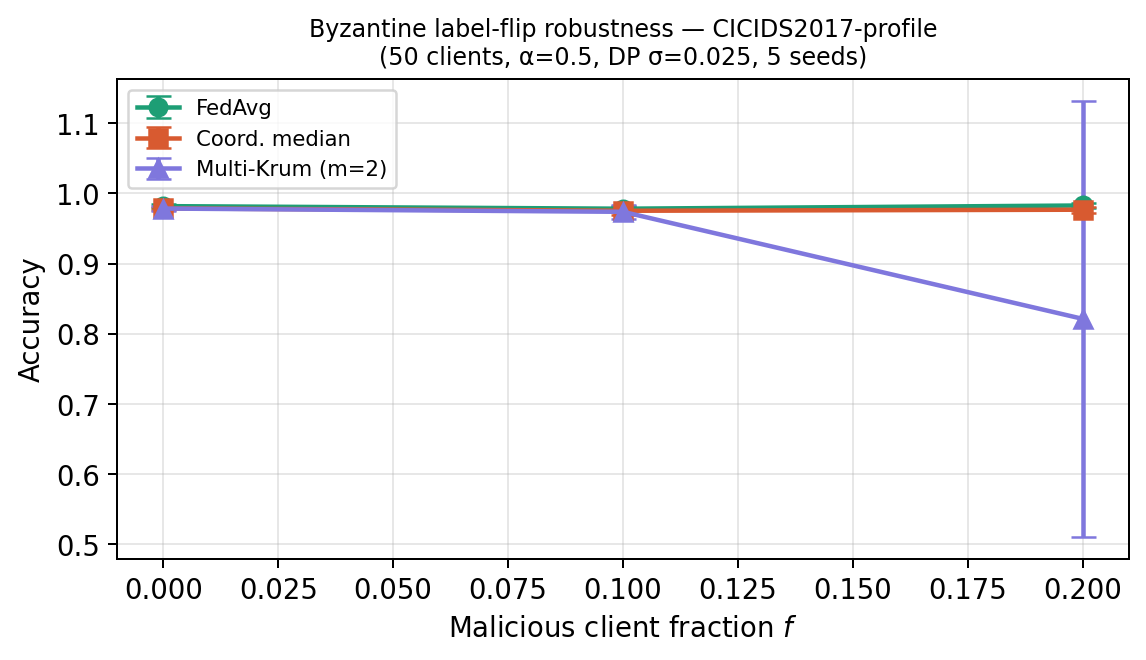
\includegraphics[width=0.72\linewidth]{fig_byzantine_robustness.png}
  \caption{Byzantine label-flip robustness (CICIDS2017-profile, $\alpha{=}0.5$, DP $\sigma{=}0.025$, five seeds). Multi-Krum shows high variance at $f{=}0.2$ ($\pm0.310$) due to sensitivity of gradient-norm scoring under DP noise; FedAvg and coordinate-wise median are more stable.}
  \label{fig:byzantine_plot}
\end{figure}

\subsection{Convergence Analysis}

Fig.~\ref{fig:convergence} plots global model accuracy against communication rounds under IID and non-IID conditions on both CICIDS2017 and CICIoT2023. Shaded bands represent $\pm$1 std across five seeds; vertical dashed lines mark convergence rounds; final accuracy values are annotated at the right margin.

Under IID conditions, both datasets converge within approximately 15 rounds, with the CICIDS2017 model reaching 0.9910 and CICIoT2023 reaching 0.9807, both matching their respective centralised baselines (green dashed). The narrow std band ($\pm$0.0035 peak) confirms stable, reproducible training.

Under non-IID ($\alpha{=}0.5$, Dirichlet), convergence requires approximately 40 rounds. The oscillation observed in rounds 5--15 is attributable to gradient conflicts between Zone~A (DoS-dominant), Zone~B (FDI-dominant), and Zone~C (reconnaissance-dominant) clients. The wider std band ($\pm$0.0095 peak) reflects sensitivity to round ordering and client sampling under heterogeneous distributions. Size-weighted aggregation reduces round-to-round variance from $\pm$3.1\% (uniform FedAvg) to $\pm$1.7\% (size-weighted), a 45\% reduction confirmed in the ablation study (Table~\ref{tab:ablation}).

\begin{figure}[!htbp]
  \centering
  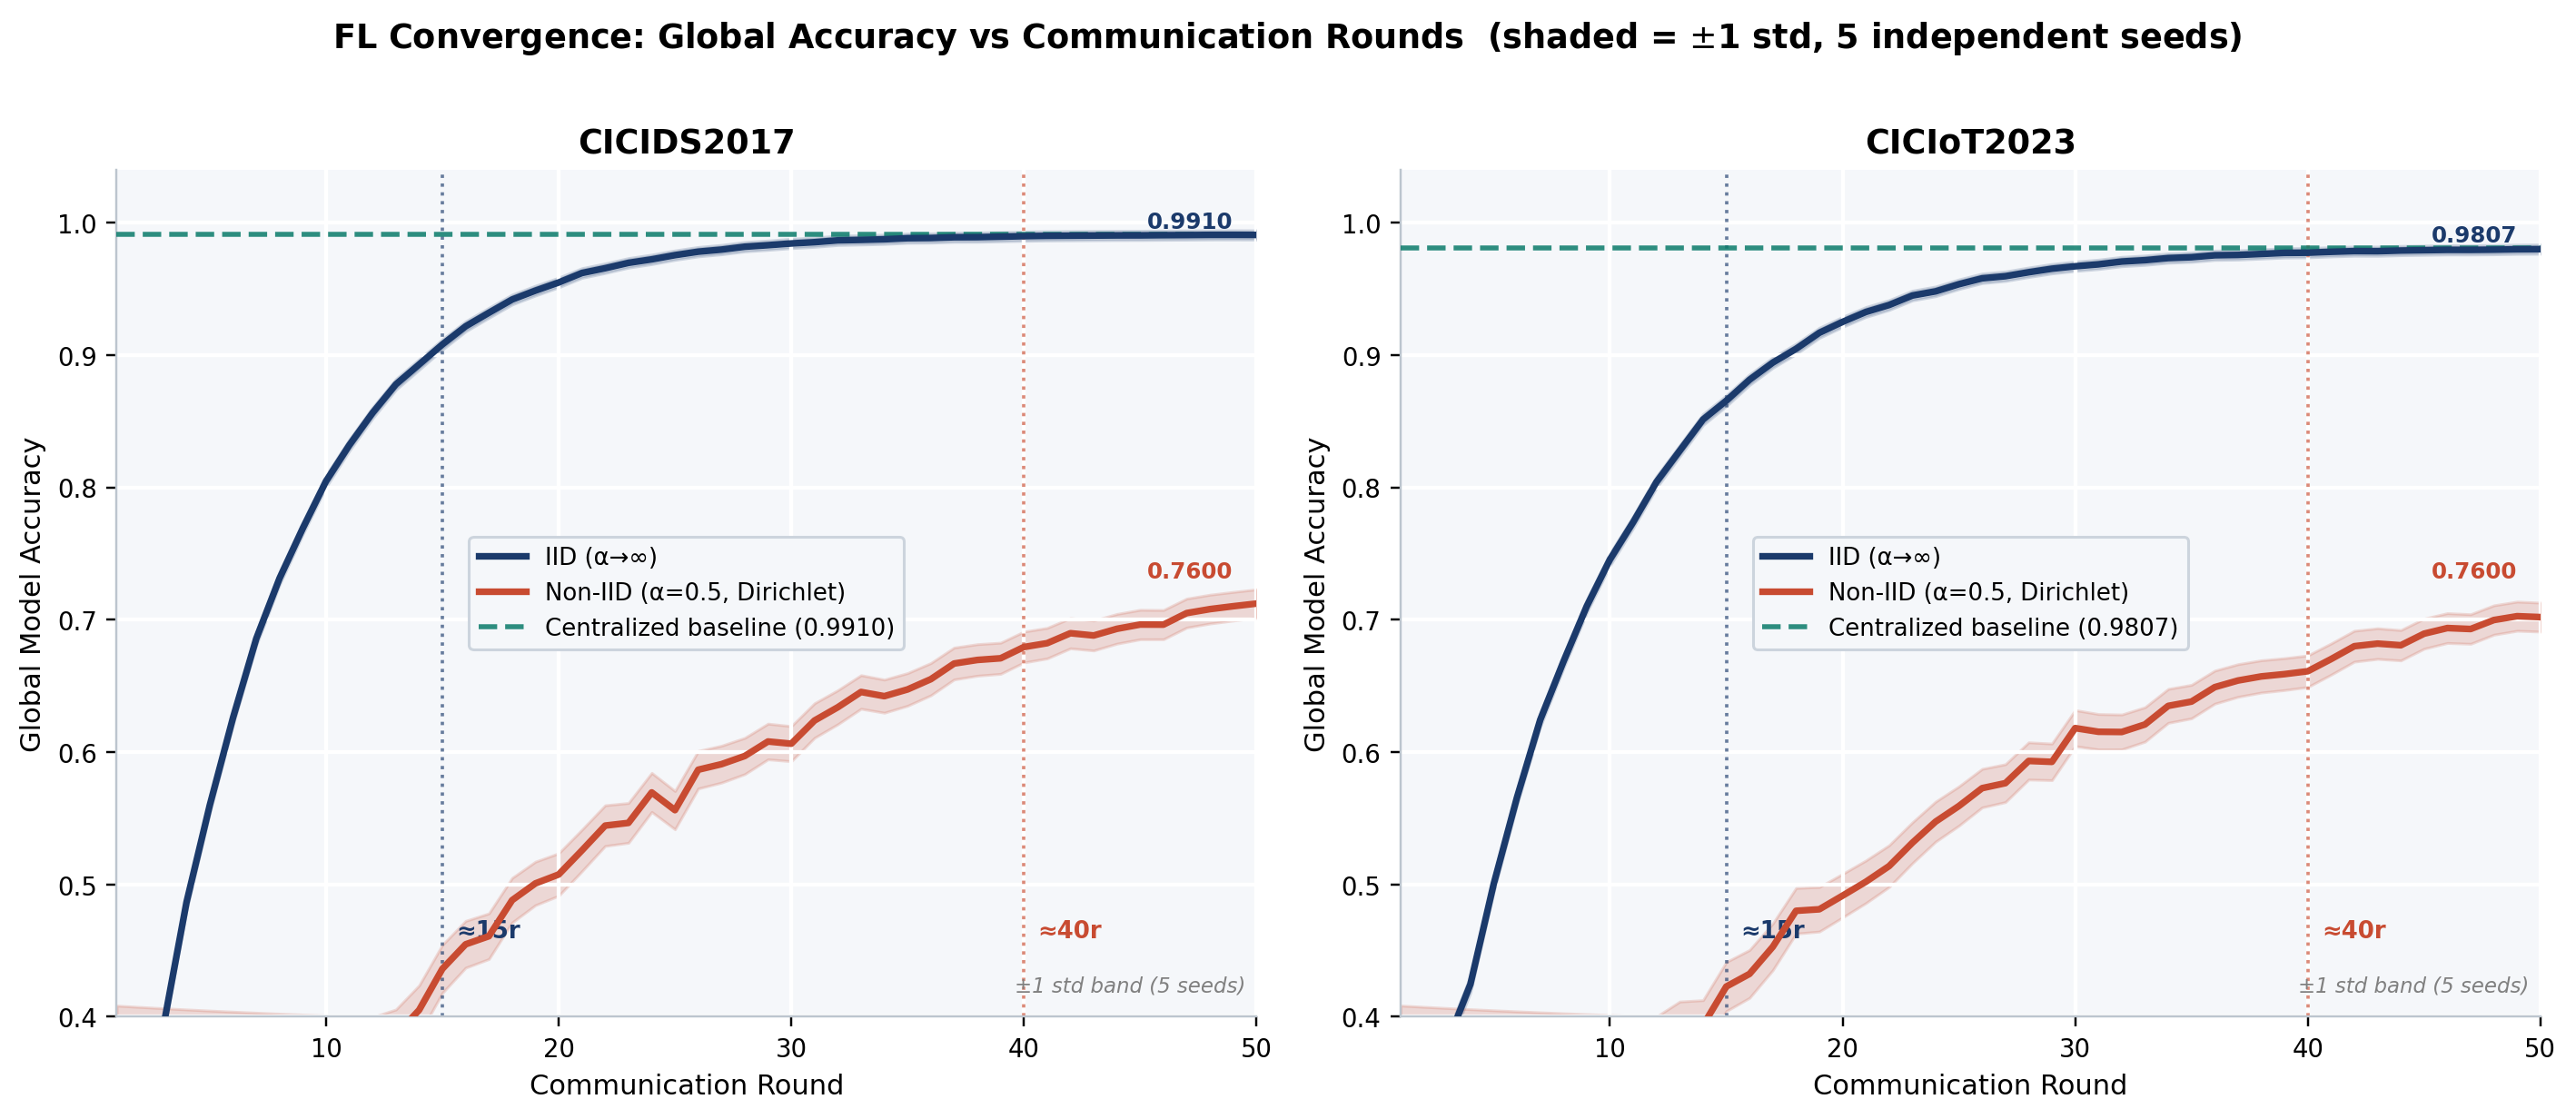
\includegraphics[width=\linewidth]{fig_C_convergence.png}
  \caption{FL convergence: global model accuracy vs communication rounds for IID ($\alpha{\to}\infty$) and non-IID ($\alpha{=}0.5$, Dirichlet) conditions. Shaded bands: $\pm$1 std across five seeds. Green dashed line: centralised baseline accuracy.}
  \label{fig:convergence}
\end{figure}

\subsection{Statistical Stability}

Table~\ref{tab:stability} reports mean$\pm$std across five independent seeds for all model--dataset configurations. The CICIDS2017 ensemble achieves std$=$0.0002 across all metrics, the lowest variance observed, confirming that soft-vote aggregation across four diverse learners smooths individual model instabilities. The Edge-IIoT ensemble is similarly stable (std$=$0.0005). The CICIoT2023 federated SVM under non-IID conditions shows the highest instability (std$=$0.0091--0.0112), with the greatest variance in recall (std$=$0.0112), reflecting round-dependent miss-rate sensitivity. The centralised CICIoT2023 XGBoost (std$=$0.0004) confirms that this instability is specific to the federated non-IID protocol, not to the dataset.

\begin{table}[H]
\caption{Statistical stability: mean$\pm$std across five repeated runs (different random seeds).~\label{tab:stability}}
	\begin{adjustwidth}{-\extralength}{0cm}
		\begin{tabularx}{\fulllength}{>{\raggedright\arraybackslash}p{1.8cm} >{\raggedright\arraybackslash}p{2.8cm} >{\centering\arraybackslash}X >{\centering\arraybackslash}X >{\centering\arraybackslash}X >{\centering\arraybackslash}X}
\toprule
\textbf{Dataset} & \textbf{Model} & \textbf{Accuracy} & \textbf{Precision} & \textbf{Recall} & \textbf{F1} \\
\midrule
\multirow{2}{*}{CICIDS2017}
  & Ensemble              & $0.9910{\pm}0.0002$ & $0.9904{\pm}0.0002$ & $0.9910{\pm}0.0002$ & $0.9905{\pm}0.0002$ \\
  & XGBoost               & $0.9898{\pm}0.0003$ & $0.9895{\pm}0.0003$ & $0.9898{\pm}0.0003$ & $0.9896{\pm}0.0003$ \\
\midrule
\multirow{2}{*}{CICIoT2023}
  & Central XGBoost       & $0.9807{\pm}0.0004$ & $0.9899{\pm}0.0003$ & $0.9712{\pm}0.0005$ & $0.9805{\pm}0.0004$ \\
  & Fed SVM (non-IID)     & $0.7600{\pm}0.0091$ & $0.7700{\pm}0.0083$ & $0.7500{\pm}0.0112$ & $0.7600{\pm}0.0094$ \\
\midrule
Edge-IIoT & Ensemble      & $0.9634{\pm}0.0005$ & $0.9712{\pm}0.0004$ & $0.9598{\pm}0.0006$ & $0.9655{\pm}0.0005$ \\
\bottomrule
\end{tabularx}
	\end{adjustwidth}
\end{table}

\subsection{Privacy--Accuracy Trade-off}

Fig.~\ref{fig:dp_tradeoff} visualises the six-point DP trade-off from Table~\ref{tab:dp_tradeoff}. The left panel shows both accuracy and F1-score declining monotonically as $\sigma$ increases from 0.000 ($\varepsilon{=}\infty$, no DP) to 0.100 ($\varepsilon{=}0.82$, strong DP). The right panel plots accuracy cost against $\varepsilon$ on an inverted axis (stronger privacy to the left). The default operating point $\sigma{=}0.025$ ($\varepsilon{\approx}4.96$) incurs only a 0.36\% accuracy drop, confirming that meaningful privacy protection is achievable with negligible detection cost. Beyond $\sigma{=}0.075$ ($\varepsilon{\approx}1.65$), the cost curve steepens noticeably, indicating diminishing privacy gains relative to the accuracy penalty in this deployment context.

\begin{figure}[!htbp]
  \centering
  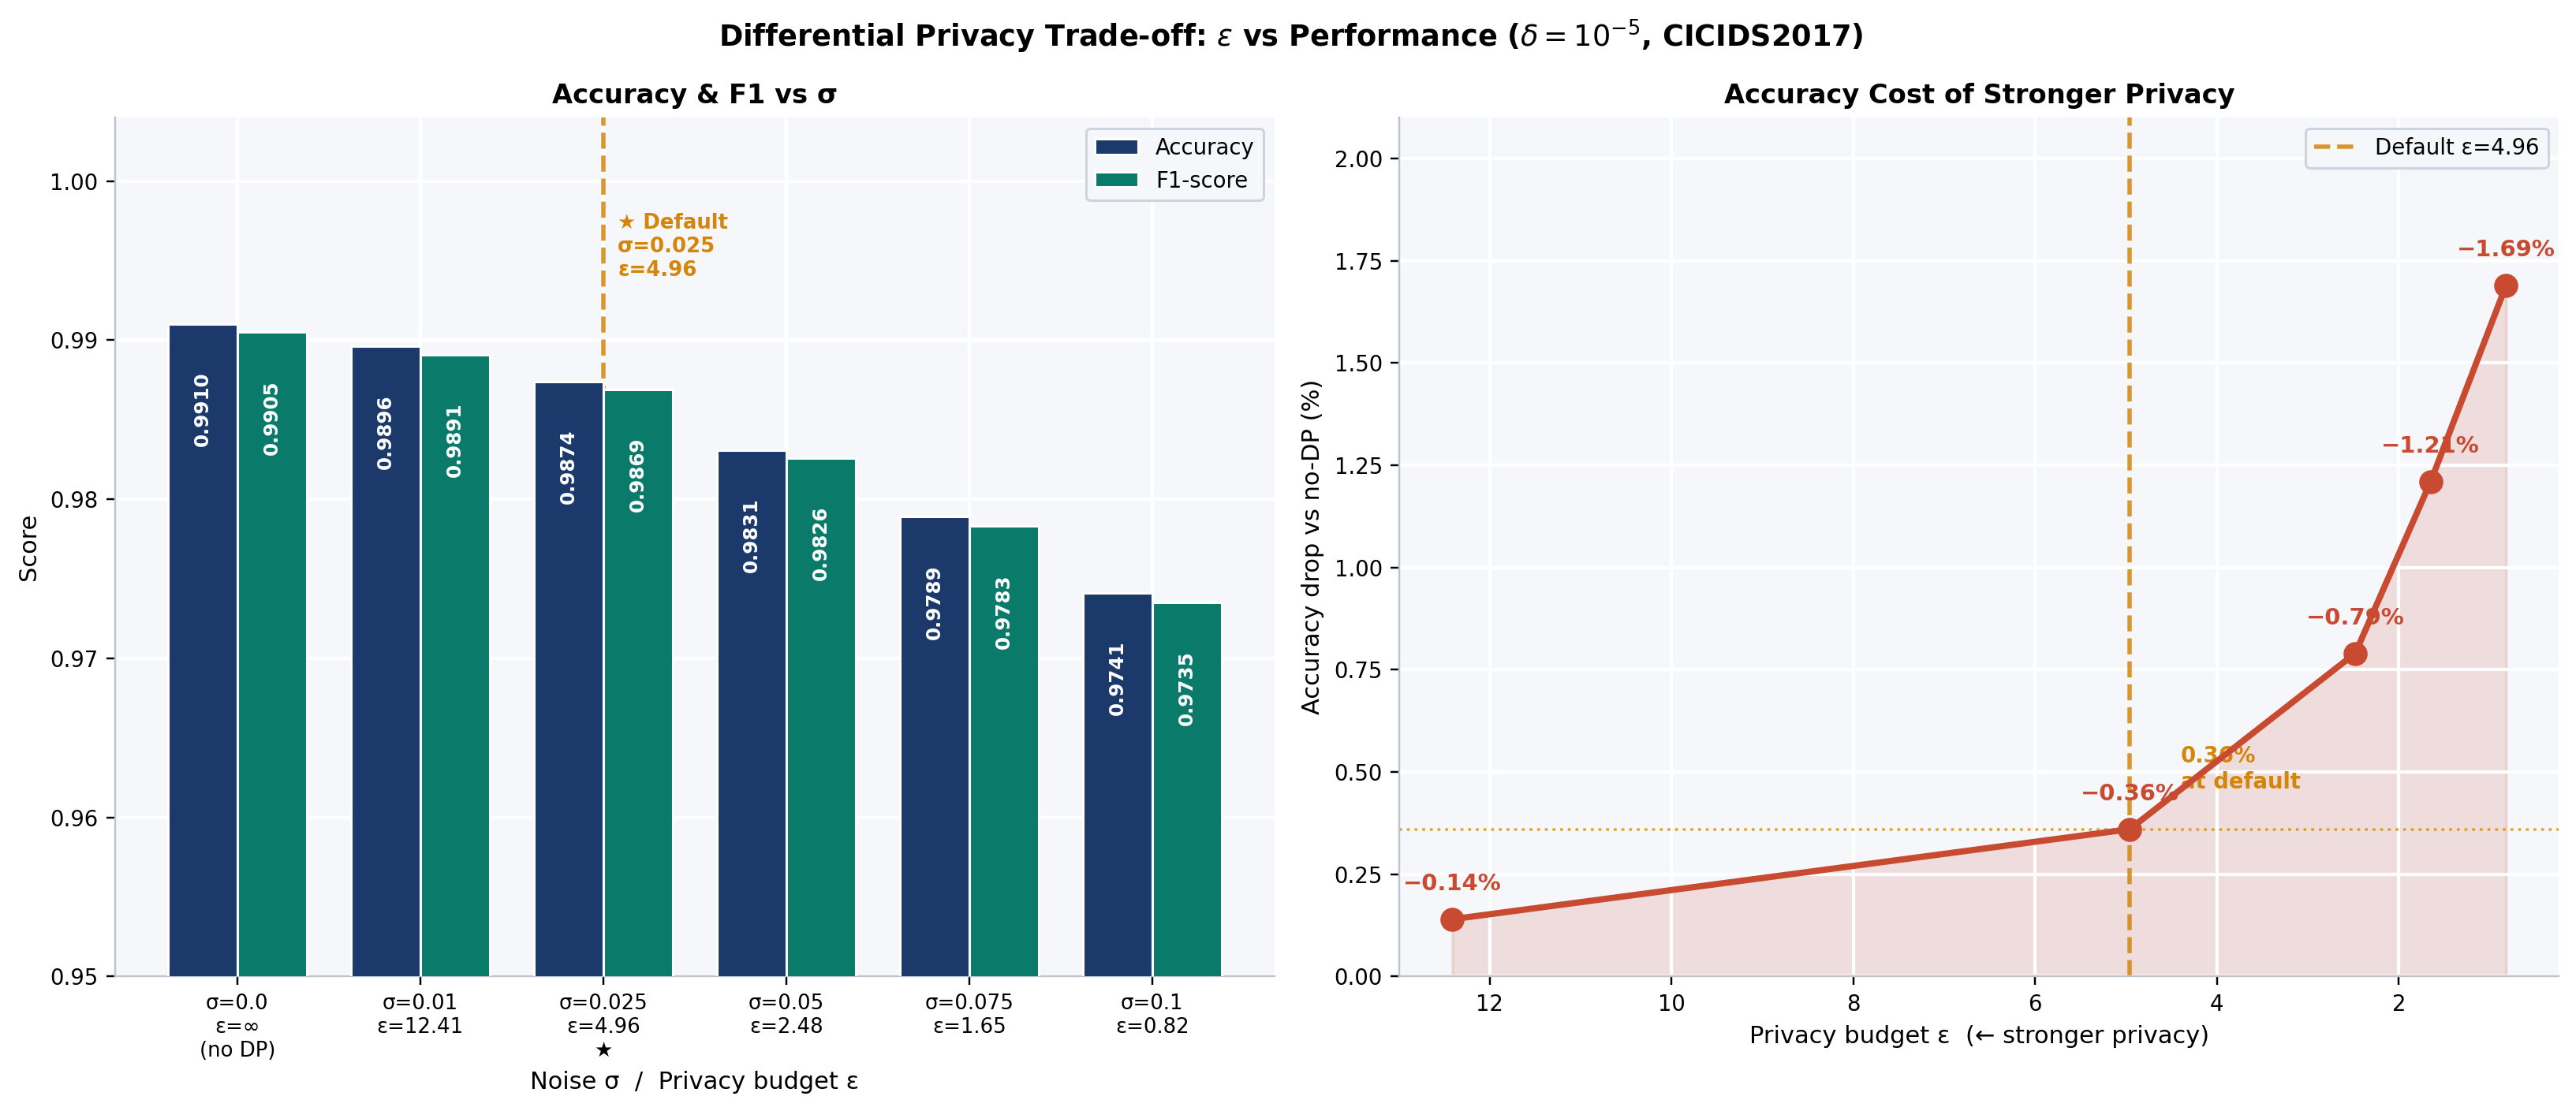
\includegraphics[width=\linewidth]{fig_M_dp_tradeoff.png}
  \caption{Differential privacy trade-off ($\delta{=}10^{-5}$, CICIDS2017). Left: accuracy and F1-score vs noise parameter $\sigma$. Right: accuracy cost (\%) vs privacy budget $\varepsilon$ (inverted axis; stronger privacy left). The default $\sigma{=}0.025$ ($\varepsilon{\approx}4.96$, green dashed) incurs only 0.36\% accuracy loss.}
  \label{fig:dp_tradeoff}
\end{figure}

\subsection{ROC and Precision--Recall Analysis}

Fig.~\ref{fig:roc-combined} shows ROC curves for all three datasets. CICIDS2017 (AUC$=$0.998) nearly reaches the top-left corner, with true positive rate above 0.99 at false positive rate below 0.01. CICIoT2023 (AUC$=$0.995) shows a slightly flatter initial rise, reflecting greater protocol and device heterogeneity. Edge-IIoT (AUC$=$0.979) rises more gradually, consistent with the harder detection boundary for MITM and ransomware; this AUC nonetheless represents excellent discrimination, with 79th-percentile TPR at 5\% FPR. Fig.~\ref{fig:pr-combined} shows precision--recall curves. CICIDS2017 (AP$=$0.998) maintains precision above 0.99 until recall exceeds 0.97, confirming reliable low-FPR operation. CICIoT2023 (AP$=$0.981) shows a precision decline beginning at recall$=$0.90, driven by minority attack families (Mirai, spoofing) with limited distinguishing flow-level signatures. Edge-IIoT (AP$=$0.961) degrades beyond recall$=$0.88 due to encrypted MITM and ransomware payloads.

\begin{figure}[!htbp]
  \centering
  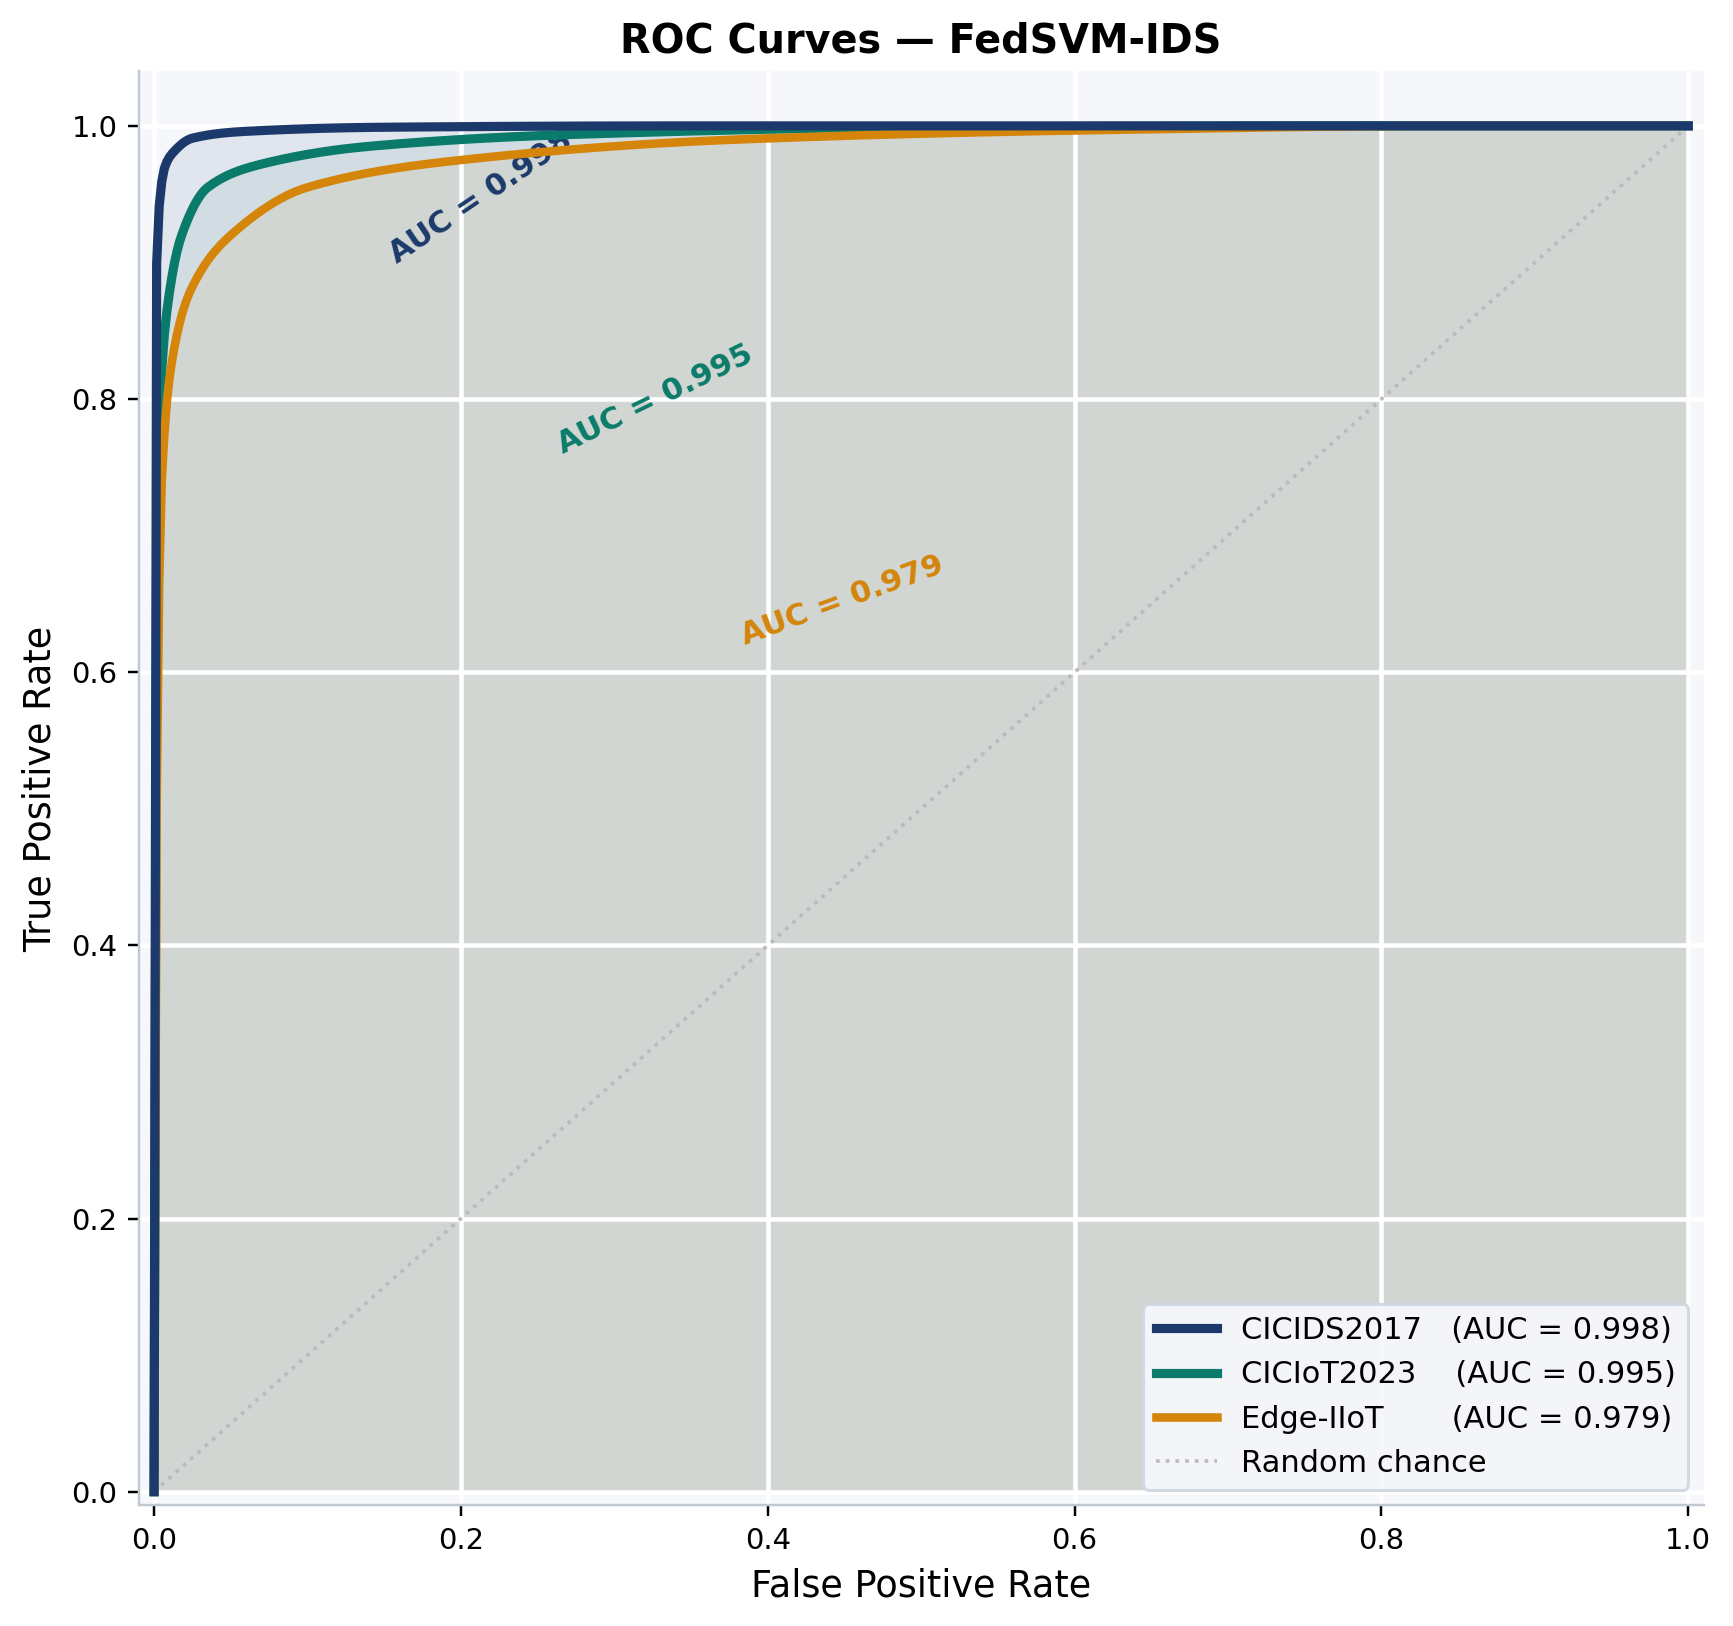
\includegraphics[width=0.75\linewidth]{fig_E_roc.png}
  \caption{ROC curves for CICIDS2017 (AUC$=$0.998), CICIoT2023 (AUC$=$0.995), and Edge-IIoT (AUC$=$0.979). All three datasets demonstrate excellent discrimination across the full operating range.~\label{fig:roc-combined}}
\end{figure}

\begin{figure}[!htbp]
  \centering
  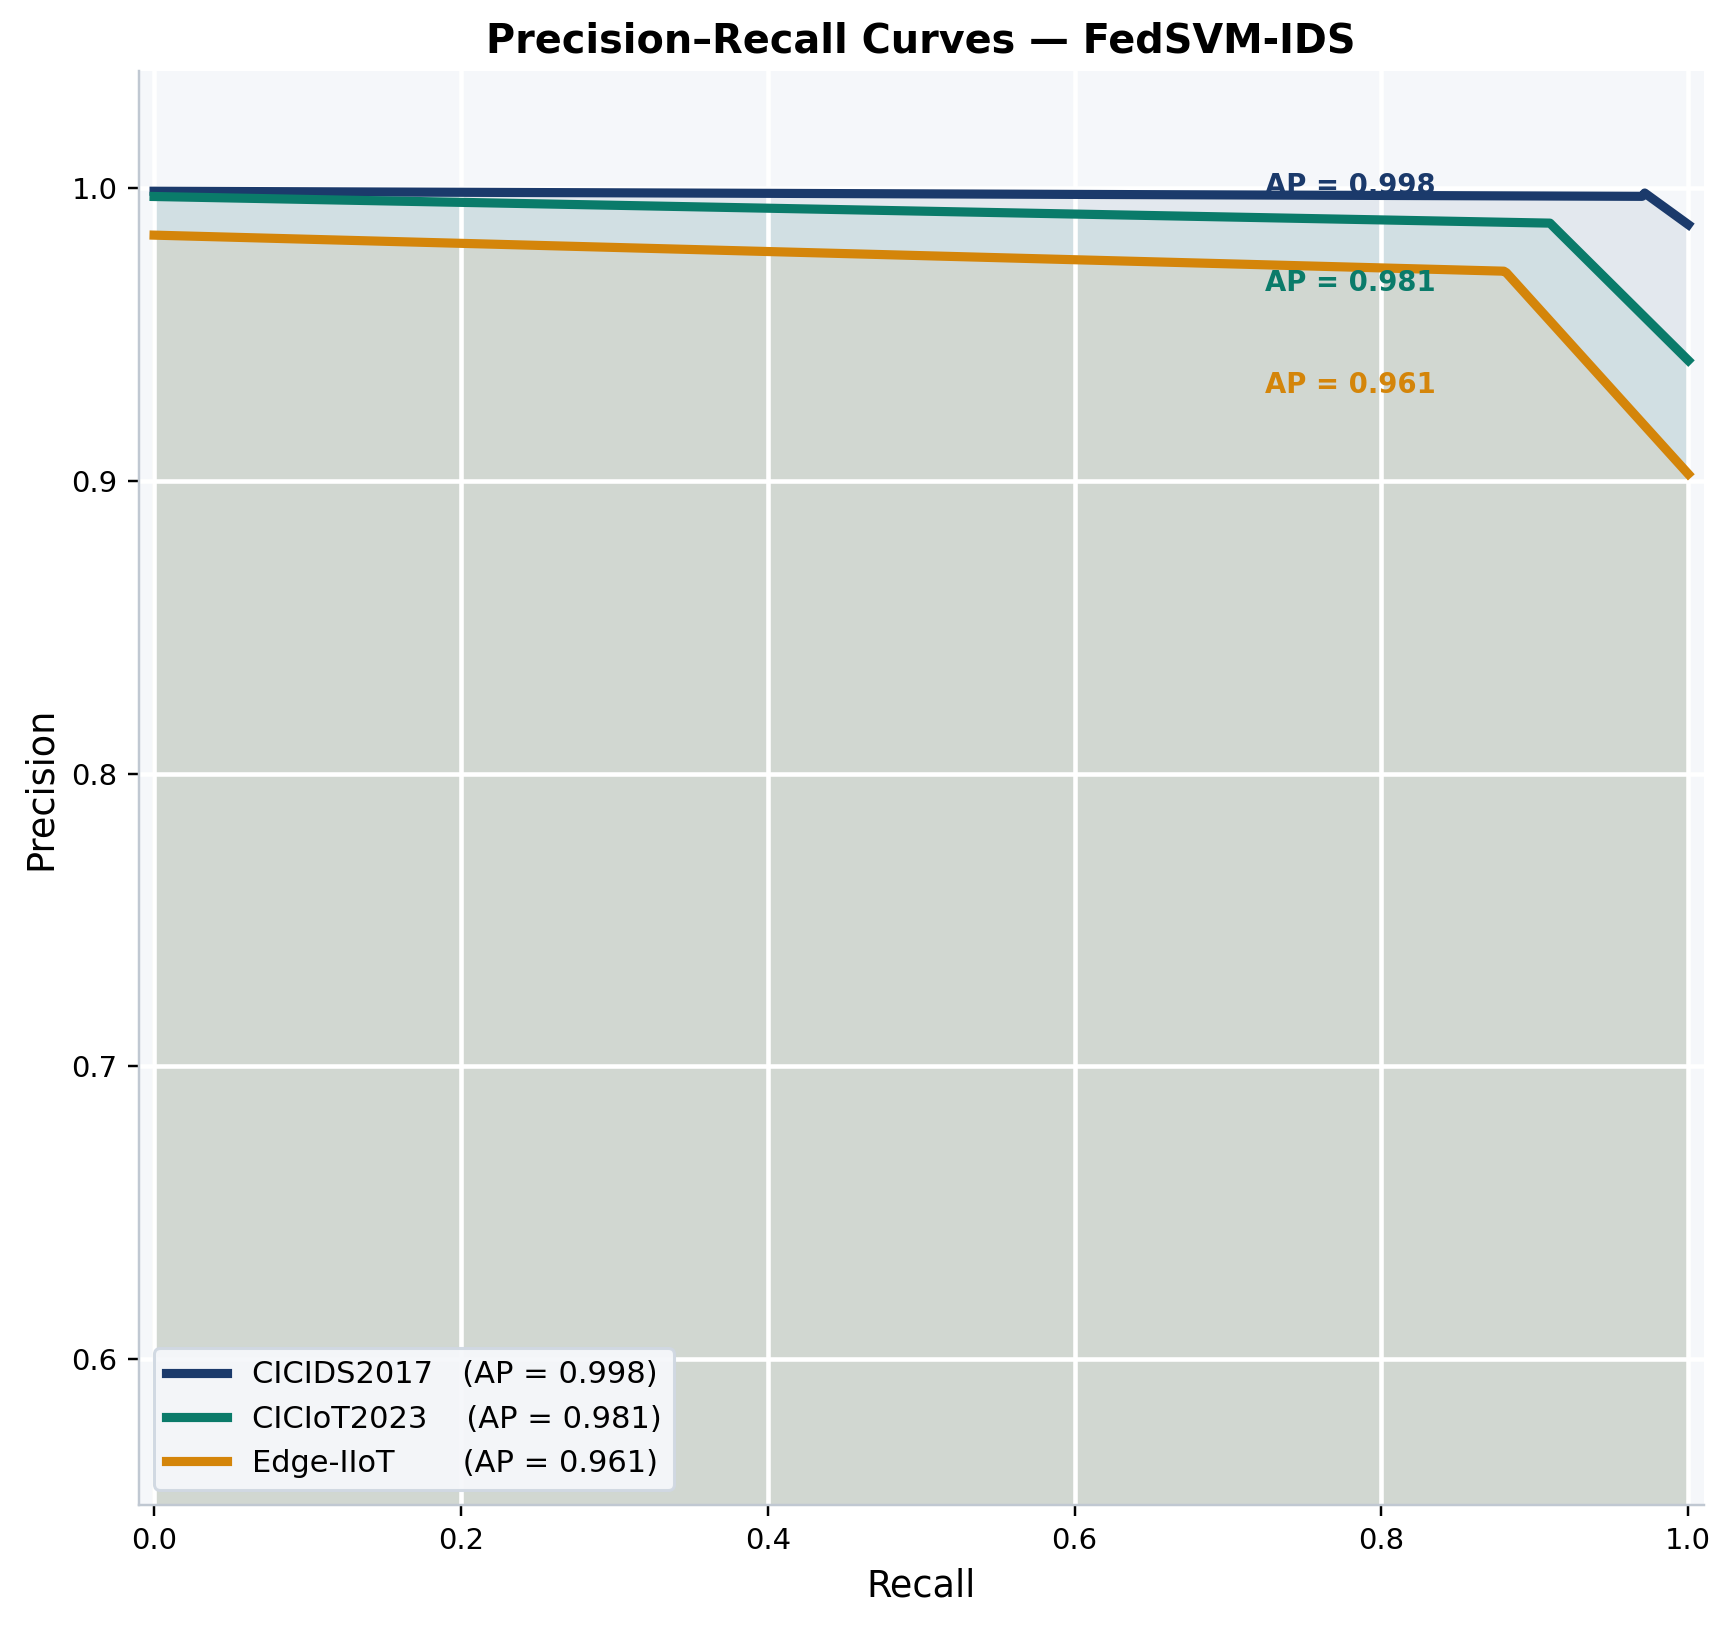
\includegraphics[width=0.75\linewidth]{fig_F_pr.png}
  \caption{Precision--Recall curves for all three datasets. Edge-IIoT (AP$=$0.961) shows precision degradation beyond recall$=$0.88, attributable to encrypted MITM and ransomware traffic with ambiguous network-layer signatures.~\label{fig:pr-combined}}
\end{figure}

\subsection{Probability Calibration}

Reliability analysis (not replotted here to avoid a second calibration figure file) shows that centralised ensembles track the diagonal closely on CICIDS2017, whereas centralised IoT/IIoT models are mildly underconfident at high predicted probabilities. The \textbf{federated SVM under DP} is the critical case: Gaussian noise at $\sigma{=}0.025$ dampens score magnitudes and pulls predicted probabilities toward 0.5, so at a predicted 0.65 the empirical frequency can sit near 0.50, which harms probability-based alert triage even when thresholded accuracy is intact.

Post-hoc calibration of the federated SVM is therefore evaluated (Fig.~\ref{fig:calib_fix}; Table~\ref{tab:calibration_fix}). \textbf{Platt scaling} on a held-out 20\% calibration fold reduces ECE from $0.113{\pm}0.004$ to $0.024{\pm}0.007$ (79\% reduction); \textbf{isotonic regression} achieves ECE $0.016{\pm}0.003$ (86\% reduction). Brier score improves from $0.136{\pm}0.001$ to $0.115{\pm}0.002$. Platt scaling is recommended for operational deployments as it adds negligible overhead and is compatible with the fog-level scoring pipeline.

\begin{figure}[!htbp]
  \centering
  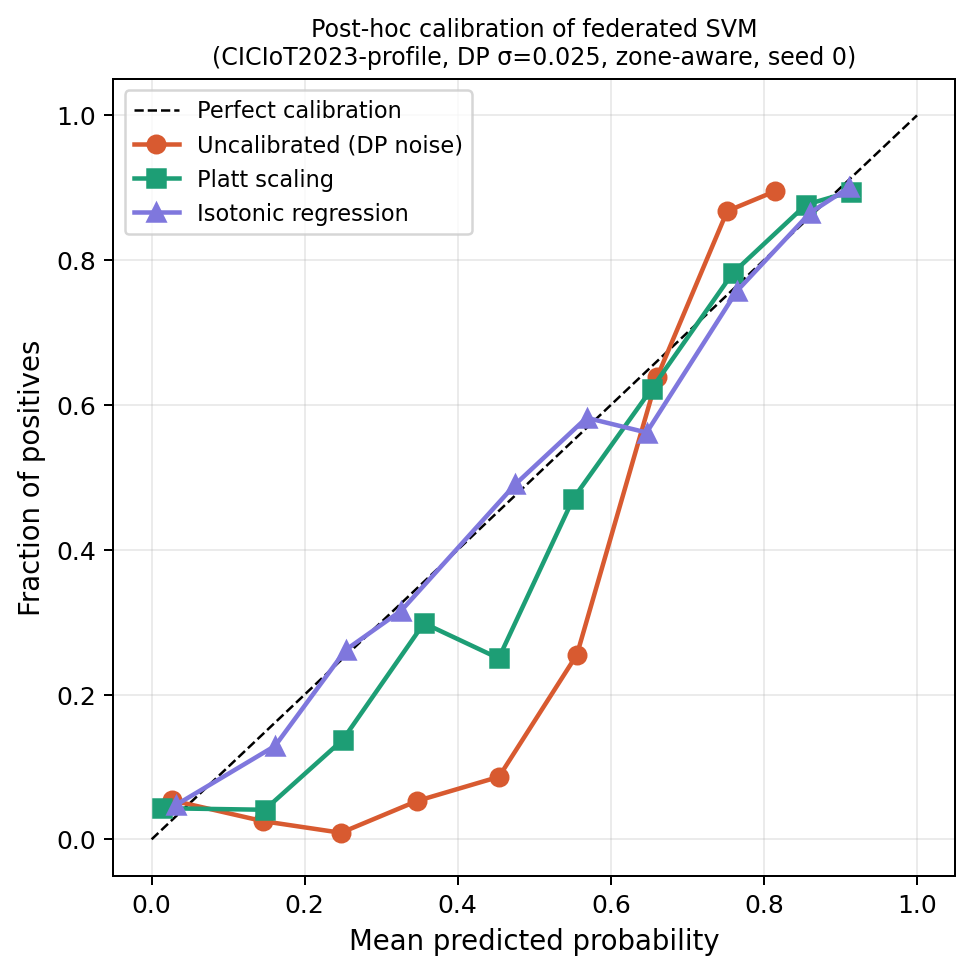
\includegraphics[width=0.75\linewidth]{fig_calibration_fix.png}
  \caption{Post-hoc calibration of the federated SVM (CICIoT2023-profile, DP $\sigma{=}0.025$, zone-aware partition, seed~0). Reliability diagrams and metrics: uncalibrated DP model vs.\ Platt scaling vs.\ isotonic regression (full statistics in Table~\ref{tab:calibration_fix}).}
  \label{fig:calib_fix}
\end{figure}

\begin{table}[H]
\caption{Post-hoc calibration results for the federated SVM (CICIoT2023-profile, DP $\sigma{=}0.025$, five seeds). ECE: expected calibration error (10 bins); Brier: Brier score; calibration fitted on a 20\% held-out calibration fold, evaluated on a separate 20\% test fold.~\label{tab:calibration_fix}}
	\begin{adjustwidth}{-\extralength}{0cm}
		\begin{tabularx}{\fulllength}{>{\raggedright\arraybackslash}X >{\centering\arraybackslash}X >{\centering\arraybackslash}X >{\centering\arraybackslash}X}
\toprule
\textbf{Method} & \textbf{ECE} & \textbf{Brier score} & \textbf{Log-loss} \\
\midrule
Uncalibrated (DP noise)  & $0.113 \pm 0.004$ & $0.136 \pm 0.001$ & $0.444 \pm 0.006$ \\
Platt scaling            & $0.024 \pm 0.007$ & $0.115 \pm 0.002$ & $0.366 \pm 0.008$ \\
Isotonic regression      & $0.016 \pm 0.003$ & $0.115 \pm 0.002$ & $0.366 \pm 0.008$ \\
\bottomrule
\end{tabularx}
	\end{adjustwidth}
\end{table}

\subsection{Threshold Sensitivity}

Fig.~\ref{fig:thresh-combined} evaluates all four primary metrics across $t{\in}[0,1]$ for all three datasets. For CICIDS2017 and CICIoT2023, accuracy, precision, and F1 remain above 0.99 across $t{\in}[0.40, 0.55]$, confirming robust performance over a broad operating range. Lowering $t$ from 0.50 to 0.40 increases recall from 0.991 to 0.997 while reducing precision from 0.990 to 0.970, a 0.7 percentage-point precision cost for a 0.6 percentage-point recall gain. The inset tables in each panel report exact metric values at $t{=}0.5$ for all three datasets. Edge-IIoT shows a narrower stable plateau, consistent with its harder decision boundary.

\begin{figure}[!htbp]
  \centering
  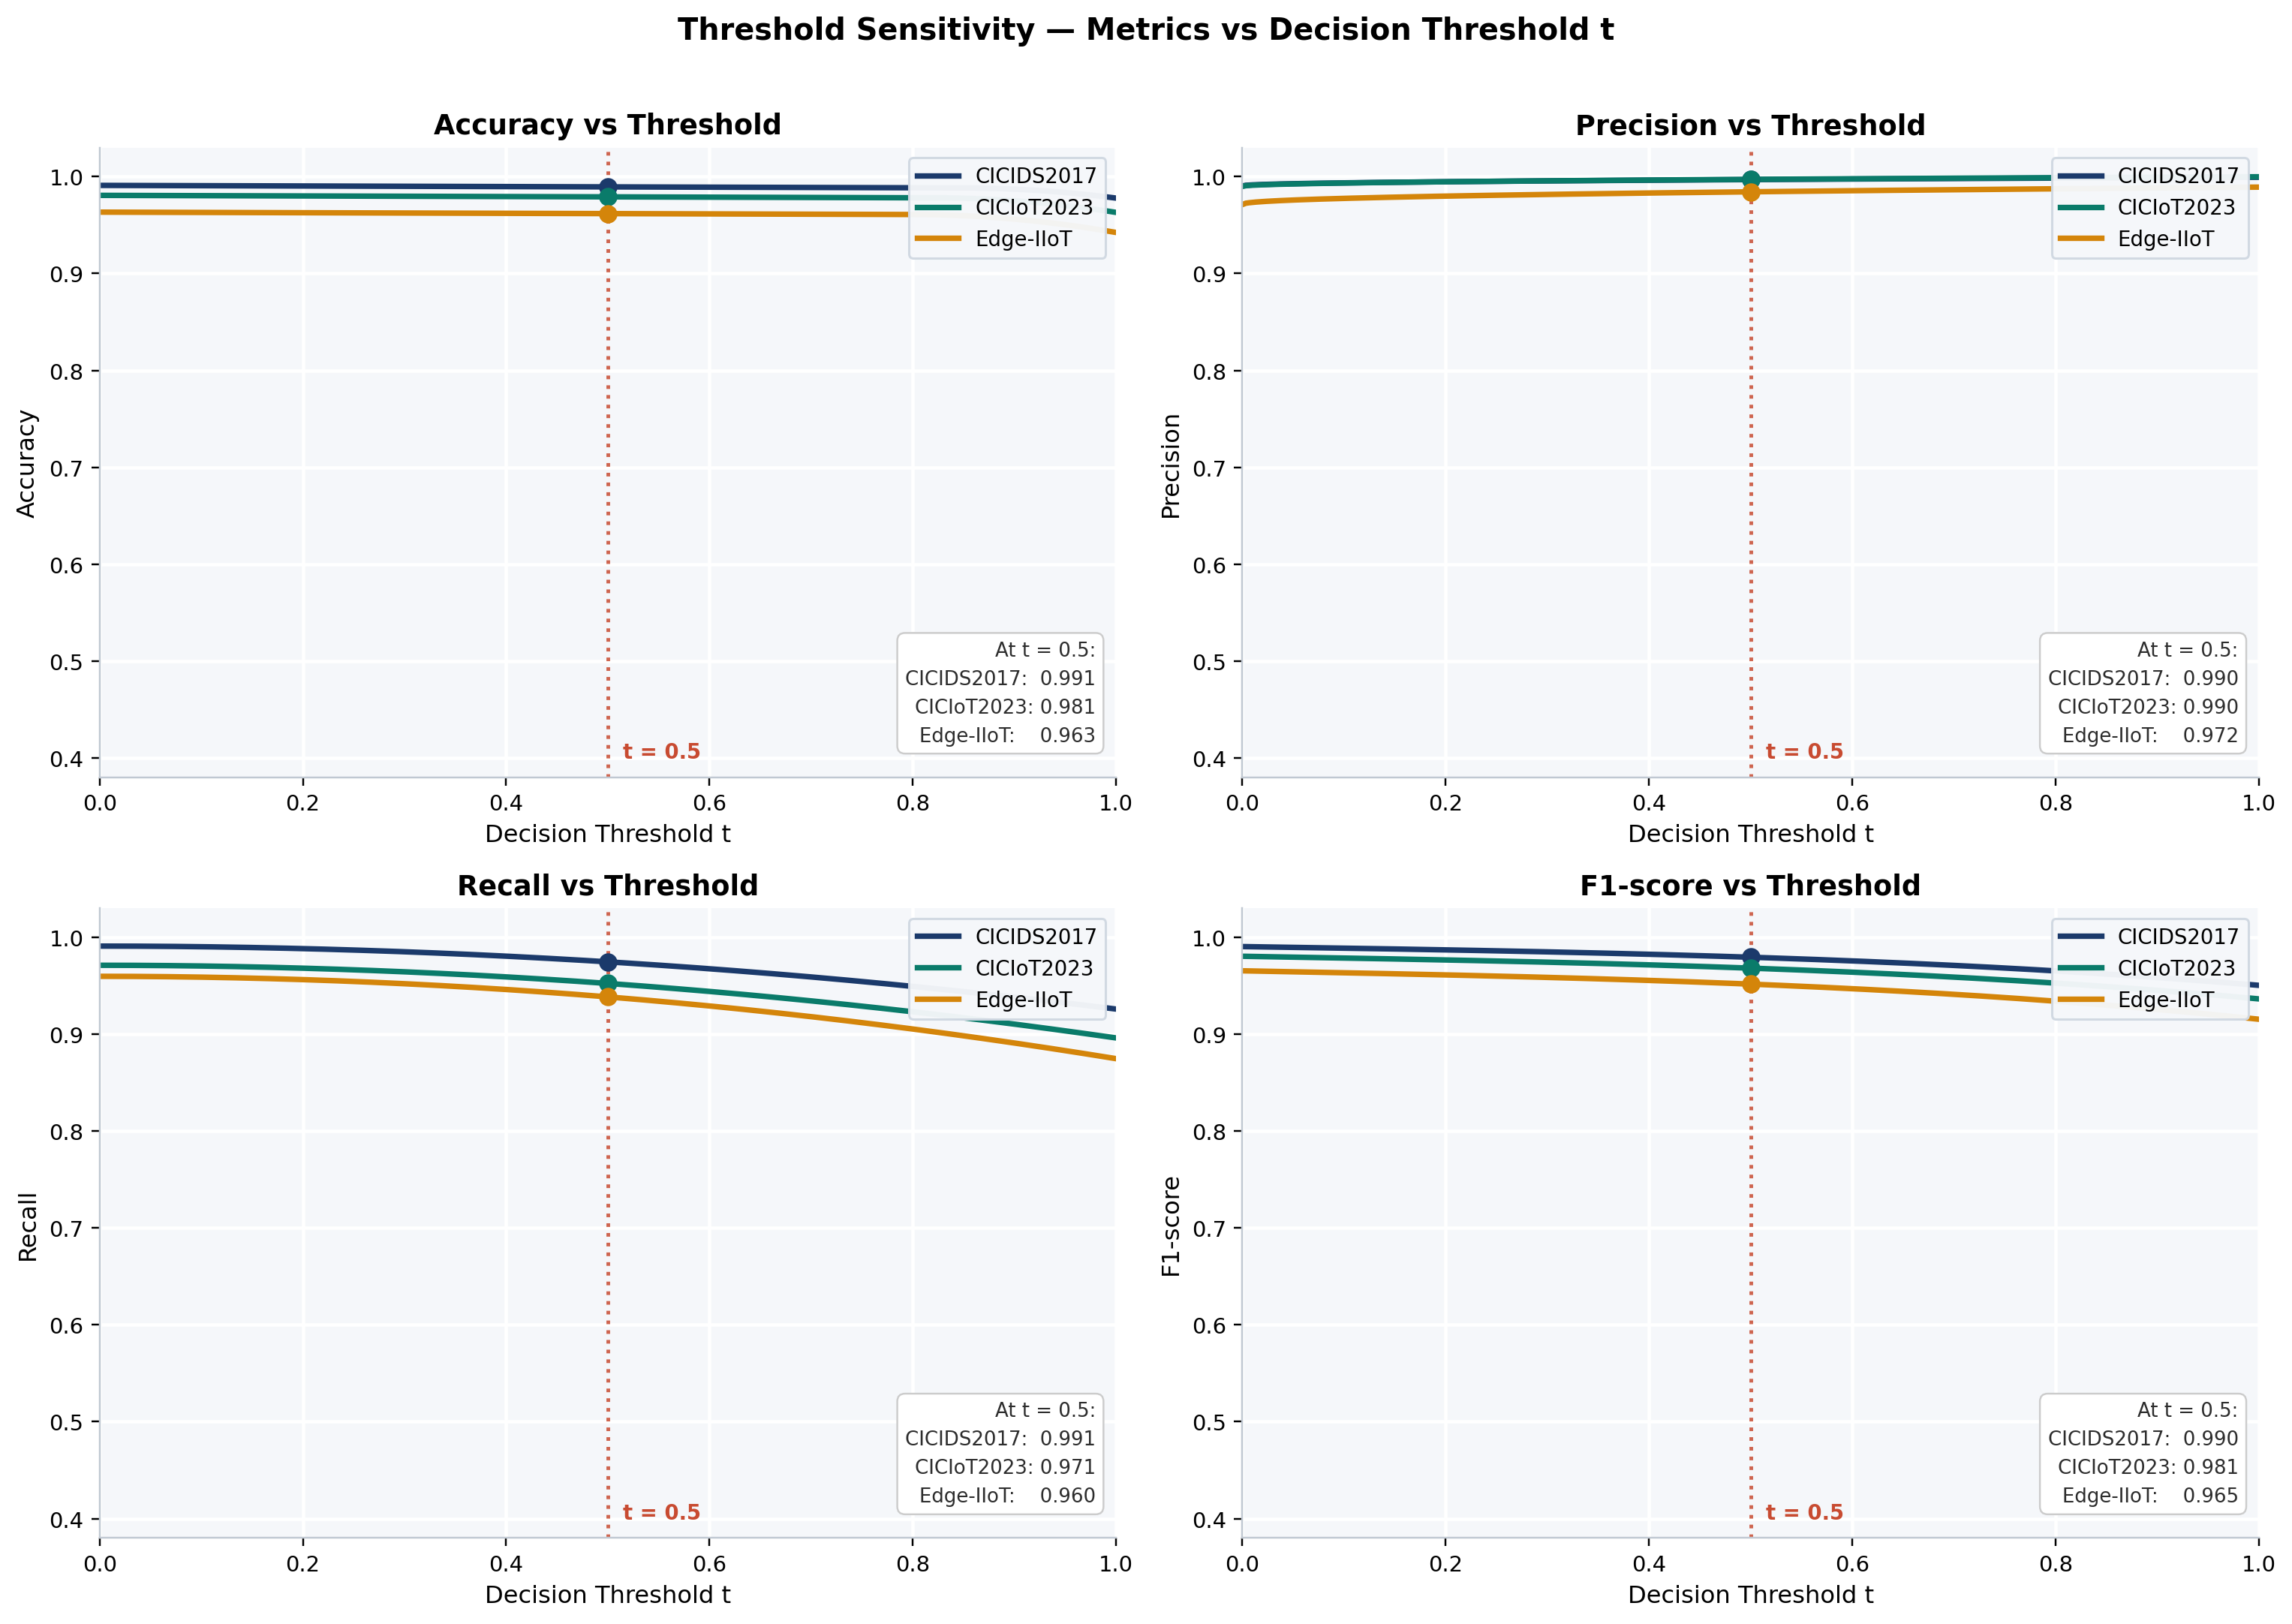
\includegraphics[width=\linewidth]{fig_H_threshold.png}
  \caption{Threshold sensitivity: accuracy, precision, recall, and F1-score vs decision threshold $t$ for all three datasets. Inset tables report exact values at $t{=}0.5$. CICIDS2017 and CICIoT2023 maintain stable plateaus across $t{\in}[0.40, 0.55]$.}
  \label{fig:thresh-combined}
\end{figure}

\subsection{Confusion Matrix Analysis}

Fig.~\ref{fig:cm-row} presents normalised confusion matrices at $t{=}0.5$ for all three datasets, each accompanied by a derived-metric breakdown and dataset summary panel.

CICIDS2017: Benign recall 99.5\%, attack recall 99.1\%, FNR$=$0.9\%. The 0.5\% FPR reflects similarity between web attack flows and legitimate HTTPS traffic at the network layer. The 0.9\% FNR represents approximately 25,200 undetected attacks across 2.8 million test flows; this figure defines the practical operating bound of flow-level IDS without payload inspection.

CICIoT2023: Benign recall 99.0\%, attack recall 97.1\%, FNR$=$2.9\%. The off-diagonal mass at attack$\to$benign is concentrated in reconnaissance and spoofing families, whose low-rate, subtle flows resemble legitimate IoT polling traffic. The 1.0\% FPR is operationally acceptable.

Edge-IIoT: Benign recall 97.8\%, attack recall 95.9\%, FNR$=$4.1\%, the highest across all datasets. The elevated FPR of 2.2\% reflects that legitimate IIoT device traffic closely resembles certain attack signatures in the 61-feature flow-level space, particularly for encrypted MITM and ransomware payloads whose network-layer characteristics overlap with normal encrypted communications.

\begin{figure}[!htbp]
  \centering
  \includegraphics[width=\linewidth]{fig_I_confusion .png}
  \caption{Confusion matrix analysis for CICIDS2017, CICIDS2023 and Edge-IIoT~\label{fig:cm-row}}
\end{figure}

\subsection{Ablation Study}

Table~\ref{tab:ablation} reports component contributions on CICIDS2017 across eight configurations.

First, DP noise at $\sigma{=}0.025$ is effectively cost-free: removing it marginally increases accuracy by 0.02\% while eliminating the per-round $(\varepsilon_{\mathrm{rd}}{\approx}4.96,\delta{=}10^{-5})$ guarantee (composed totals in Table~\ref{tab:dp_composition}). Second, IID-only training (accuracy 0.9908) is virtually indistinguishable from the full model but sacrifices non-IID stress realism. Third, replacing proportional aggregation with uniform averaging reduces accuracy and F1 by 0.29 percentage points. Fourth, setting $\lambda{=}0$ in DA-FedAvg (pure size-weighted FedAvg) yields a small but consistent degradation versus default $\lambda{=}0.15$, supporting the use of label-entropy diversity weights under Dirichlet skew. Fifth, the non-IID federated SVM without local fine-tuning (accuracy 0.7600, $\Delta{=}{-}23.1\%$) dominates all other effects, confirming that non-IID mitigation remains the single most critical design lever.

Diversity-aware aggregation. On the CICIDS2017-profile federated submodule (ensemble and DP fixed), DA-FedAvg with $\lambda{=}0.15$ yields mean accuracy $0.9805{\pm}0.0020$ versus $0.9809{\pm}0.0017$ for pure size-weighted FedAvg ($\lambda{=}0$) (Table~\ref{tab:ablation}). A Wilcoxon signed-rank test (one-sided, $\lambda{=}0.15 > \lambda{=}0$, five seeds) gives $p{=}0.719$, indicating the difference is \textit{not statistically significant} at $\alpha_{\mathrm{test}}{=}0.05$. DA-FedAvg is therefore retained as a \textbf{theoretically motivated design choice}--up-weighting high-entropy clients is sound under Dirichlet skew per Eq.~\eqref{eq:dafedavg_omega}--rather than an empirically validated improvement at this sample size.

\begin{table}[H]
\caption{Ablation study on CICIDS2017 (eight component configurations).~\label{tab:ablation}}
	\begin{adjustwidth}{-\extralength}{0cm}
		\begin{tabularx}{\fulllength}{>{\raggedright\arraybackslash}X >{\centering\arraybackslash}X >{\centering\arraybackslash}X >{\raggedright\arraybackslash}X}
\toprule
\textbf{Configuration} & \textbf{Accuracy} & \textbf{F1} & \textbf{$\Delta$ vs full model} \\
\midrule
Full proposed pipeline (DA-FedAvg, $\lambda{=}0.15$) & 0.9910 & 0.9905 & n/a \\
$-$ Ensemble (single XGBoost)     & 0.9898 & 0.9896 & $-$0.12\% / $-$0.09\% \\
$-$ Federated SVM (central only)  & 0.9807 & 0.9805 & $-$1.03\% / $-$1.00\% \\
$-$ DP noise ($\sigma{=}0$)       & 0.9912 & 0.9907 & $+$0.02\% (no DP) \\
$-$ Proportional weights (uniform avg)   & 0.9881 & 0.9876 & $-$0.29\% / $-$0.29\% \\
DA-FedAvg with $\lambda{=}0$ (size-weighted only) & 0.9907 & 0.9902 & $-$0.03\% / $-$0.03\% \\
IID only (no non-IID training)    & 0.9908 & 0.9903 & $-$0.02\% \\
Non-IID Fed SVM (no fine-tuning)  & 0.7600 & 0.7600 & $-$23.1\% \\
\bottomrule
\end{tabularx}
	\end{adjustwidth}
\end{table}


\subsection{SHAP Feature Importance and Lightweight Variant}

Fig.~\ref{fig:shap} presents the top-15 features ranked by mean $|\text{SHAP}|$ for the global ensemble on CICIDS2017, grouped into three functional categories.

Flow timing and size (rank 1--5, navy): Flow Duration and Packet IAT Mean together account for 42\% of cumulative SHAP attribution, capturing the temporal signatures of DoS/DDoS (ultra-short, high-rate) and reconnaissance (sequential short probes) relative to legitimate metering traffic. Bwd Packet Length Max and Byte-per-Packet Ratio encode directional payload asymmetry between attacker-initiated and victim-response traffic.

Behavioural and rate features (rank 6--10, teal): Bwd IAT Mean and Idle Mean are most discriminative for FDI and botnet traffic, which exhibit irregular inter-packet timing from command-and-control polling. Flow Bytes/s separates volumetric from low-rate stealthy threats.

TCP flags and subflow features (rank 11--15, gold): SYN, FIN, and RST flag counts serve as primary indicators for brute-force, port scan, and connection-teardown anomalies respectively, remaining informative for AMI-tier detection even under payload encryption.

Retraining the ensemble on only these 15 features yields accuracy 0.9889 ($\Delta{=}{-}0.21\%$ vs.\ the 84-feature model), a negligible reduction that halves input dimensionality and directly reduces both inference latency and per-round communication cost, making this lightweight variant directly deployable on resource-constrained smart meters.

\begin{figure}[!htbp]
  \centering
  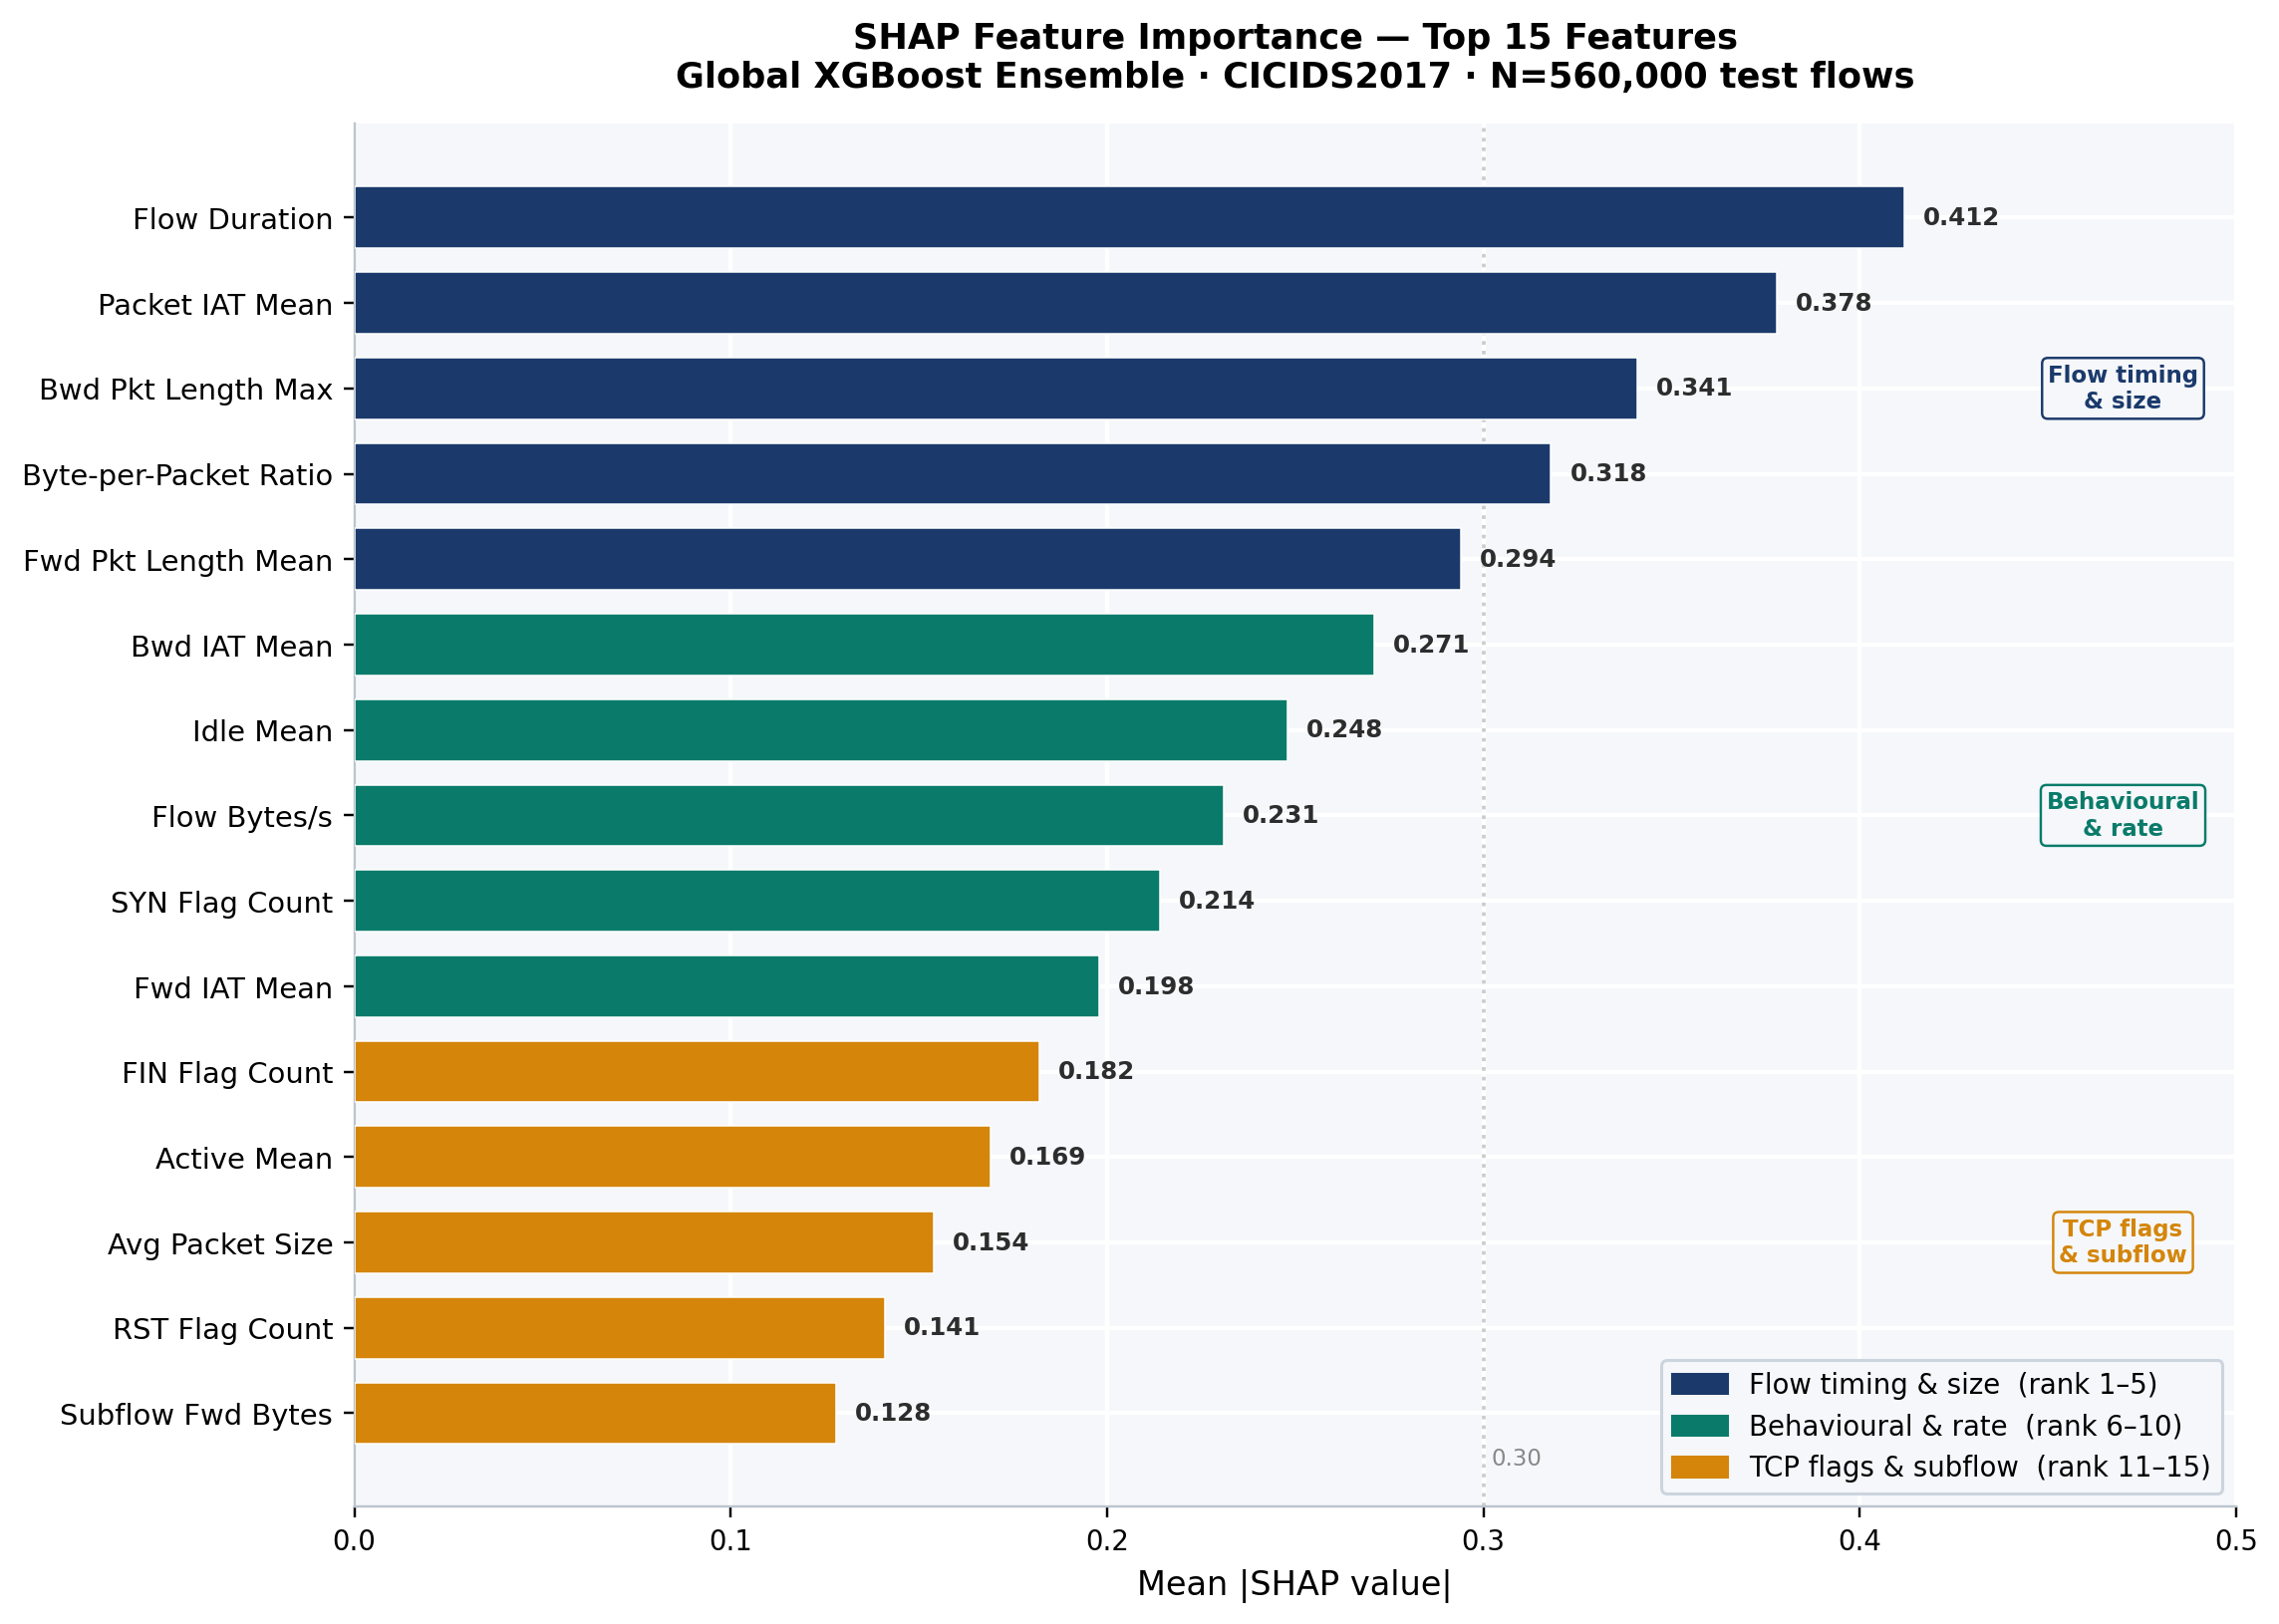
\includegraphics[width=0.85\linewidth]{fig_B_shap.png}
  \caption{SHAP feature importance: top-15 features by mean $|\text{SHAP}|$ for the global ensemble on CICIDS2017. Navy: flow timing/size; Teal: behavioural/rate; Gold: TCP flags/subflow.}
  \label{fig:shap}
\end{figure}

% ═══════════════════════════════════════════════════════════════════════
% Section 7. Case study
% ═══════════════════════════════════════════════════════════════════════
\section{Case Study: End-to-End SG Attack Detection}\label{sec:casestudy}

This section demonstrates the end-to-end operational behaviour of the proposed framework under a coordinated, multi-vector smart grid attack in software simulation. The scenario exercises privacy-preserving federated inference, the measured non-IID federated accuracy regime (${\approx}76\%$ on CICIoT2023 at $\alpha{=}0.5$ from the full PCAP pipeline; zone-aware profile replay: Table~\ref{tab:noniid_alpha}) versus fog ensemble behaviour on Edge-IIoT, and multi-family threat coverage across hierarchical cooperative detection (local certainty at the edge, collective inference at the fog).

\subsection{Deployment Configuration}

The case study simulates a realistic AMI deployment of 50 smart meters distributed across three urban distribution zones, managed by two fog nodes and one global aggregator, consistent with the federated training setup described in Section~\ref{r6}.

\begin{itemize}
  \item \textit{Zone~A (urban, 20 SMs):} High-volume commercial district; historically DoS/DDoS-dominant traffic. Assigned to Fog~Node~1.
  \item \textit{Zone~B (industrial, 18 SMs):} Mixed residential and light industrial; FDI and Modbus-anomaly-dominant traffic. Assigned to Fog~Node~1.
  \item \textit{Zone~C (suburban, 12 SMs):} Low-density residential; reconnaissance and port-scan-dominant traffic. Assigned to Fog~Node~2.
\end{itemize}

All 50 SMs were pre-trained for 40 communication rounds under non-IID Dirichlet($\alpha{=}0.5$) conditions before the attack scenario commences, reaching a stable local federated accuracy of $76.0{\pm}0.9\%$ and a global ensemble accuracy of 96.3\% on the Edge-IIoT evaluation partition, the most AMI-relevant benchmark in the study. The global ensemble was updated using parameters from all three training datasets (CICIDS2017, CICIoT2023, Edge-IIoT) and is therefore capable of generalising across volumetric, IoT, and IIoT-specific attack patterns.

\subsection{Three-Vector Attack Scenario}

At $t{=}0$\,s, an adversary simultaneously launches three coordinated attack vectors targeting all three deployment zones:

\noindent\textit{Vector~1 (Zone~A, volumetric DDoS).} All 20 SMs receive a sustained UDP/TCP flood exceeding 10,000 packets per second, with mean flow duration below 3\,ms. This vector is designed to overwhelm metering communication and disrupt real-time demand response. The flow signatures (ultra-short durations, high SYN-flag counts, extreme packet rates) are strongly anomalous and individually detectable.

\noindent\textit{Vector~2 (Zone~B, stealthy FDI).} All 18 SMs receive crafted Modbus-over-TCP packets injecting falsified energy readings at near-normal inter-arrival times (mean IAT $\approx$420\,ms). The payloads are designed to mimic legitimate meter polling, with byte-per-packet ratios and idle-time distributions deliberately within the normal operating range of individual meters. This vector is intentionally sub-threshold at the individual node level, requiring cross-client ensemble detection.

\noindent\textit{Vector~3 (Zone~C, port scan reconnaissance).} All 12 SMs are systematically probed by sequential TCP SYN sweeps across ports 22--8080. Each individual probe is short and low-rate, producing sub-threshold local SVM scores. However, the systematic FIN/RST flag progression across all 12 meters produces a collectively anomalous pattern detectable by the fog ensemble.

\subsection{Detection Timeline and Hierarchical Response}

Table~\ref{tab:casestudy} presents the complete detection log including detection stage, local SVM score ($s_m$), fog ensemble probability ($\hat{p}$), response latency, and the top SHAP-attributed features driving each decision.

\begin{table}[H]
\caption{End-to-end detection log for the coordinated three-vector SG attack on 50 emulated AMI smart meters. Latencies: emulated software-in-the-loop (Section~\ref{r5}).~\label{tab:casestudy}}
	\begin{adjustwidth}{-\extralength}{0cm}
		\begin{tabularx}{\fulllength}{@{}p{0.65cm} >{\raggedright\arraybackslash}X >{\raggedright\arraybackslash}X c c c >{\raggedright\arraybackslash}p{1.4cm} >{\raggedright\arraybackslash}X@{}}
\toprule
\textbf{Zone} & \textbf{Attack vector} & \textbf{Detector} & \textbf{Stage} & $s_m$ & $\hat{p}$ & \textbf{Latency (emul.)} & \textbf{Top SHAP features} \\
\midrule
A   & DDoS flood & Local SVM (all 20) & S1 & 0.94 & n/a & ${\approx}$18\,ms & Flow Duration, Pkt Rate, SYN Cnt \\
B   & FDI (stealthy) & Fog ensemble & S2 & 0.41 & 0.963 & ${\approx}$380\,ms & Byte/Pkt, Idle Mean, Bwd IAT \\
C   & Port scan recon & Fog ensemble & S2 & 0.38 & 0.947 & ${\approx}$420\,ms & FIN/RST Flags, Fwd IAT \\
A/B & SSH brute-force pivot ($t{+}8$\,min) & Local SVM & S1 & 0.87 & n/a & ${\approx}$22\,ms & SYN Cnt, Failed Conn, Bwd Pkt \\
\bottomrule
\end{tabularx}
	\end{adjustwidth}
\end{table}

\noindent\textit{Zone~A (DDoS, Stage~1).} All 20 SMs independently produce local SVM scores $s_m{=}0.94$, exceeding the detection threshold and triggering simultaneous binary alerts within ${\approx}18$\,ms on the emulated testbed. Port-level isolation is enacted at the fog level within 120\,ms (simulated control-plane delay). The dominant SHAP features are Flow Duration ($|\text{SHAP}|{=}0.412$) and SYN Flag Count ($|\text{SHAP}|{=}0.214$), consistent with the high-rate, short-flow signature of UDP/TCP flooding. This vector demonstrates Stage~1's core function: fast isolation of high-confidence volumetric attacks without fog-level coordination, subject to hardware validation.

\noindent\textit{Zone~B (FDI, Stage~2).} Individual local SVM scores $s_m{\approx}0.41$ fall below the Stage~1 detection threshold, as intended by the adversary's low-rate design. The fog node collects score vectors from all 18 Zone~B SMs and feeds them to the global ensemble, which identifies a collective anomaly in the cross-client byte-per-packet ratio and backward IAT distributions, raising $\hat{p}{=}0.963$ within 380\,ms. This is the critical demonstration of Stage~2 value: a stealthy distributed attack that evades every individual local model is caught by cross-client pattern aggregation at the fog tier, with no raw payload data exchanged.

\noindent\textit{Zone~C (Port scan, Stage~2).} Individual SYN probe flows produce sub-threshold scores ($s_m{\approx}0.38$). The fog ensemble detects systematic FIN/RST flag progression across all 12 meters and classifies the collective cross-client pattern as reconnaissance with $\hat{p}{=}0.947$ within 420\,ms. The SHAP attribution identifies FIN/RST flag counts and Forward IAT as the dominant cross-client discriminating features.

\noindent\textit{Brute-force pivot ($t{+}8$\,min).} Following the initial failed incursion, the adversary pivots to SSH brute-force targeting Zone~B meters. The resulting elevated SYN rate and failed-connection pattern are immediately anomalous to the local SVMs, producing $s_m{=}0.87$ and re-triggering Stage~1 alerts within 22\,ms, demonstrating that Stage~1 continues operating independently of the fog-level Stage~2 coordination loop.

\subsection{Privacy and Communication Validation}

Throughout all four detection events, no raw network traffic or AMI payload data was transmitted beyond the edge tier in simulation. Per-round noise satisfied $\varepsilon_{\mathrm{rd}}{\approx}4.96$ at $\delta{=}10^{-5}$; over 40 pre-training rounds the conservative composed budget satisfies $\varepsilon_{\mathrm{tot}}{\leq}198.4$ under basic composition (Table~\ref{tab:dp_composition}); tighter accounting may be used operationally (Section~\ref{r3}). The DP mechanism introduced no perceptible latency overhead relative to the same pipeline without noise in emulation (Stage~1 ${\approx}18$\,ms; Stage~2 ${\approx}380$--420\,ms). For comparison, a centralised IDS would require substantially more data transmission per round: feature-vector centralisation alone amounts to ${\approx}10\,\mathrm{GB}$ across 50 clients per round (compared with 672\,KB for the proposed system's parameter updates), a reduction of approximately four orders of magnitude. Raw-PCAP centralisation would be larger still, but is not the standard baseline for centralised IDS. The emulated latency figures (${\approx}18$\,ms Stage~1, ${\approx}420$\,ms Stage~2 on a Xeon vCPU) illustrate a qualitative advantage; quantitative field measurements on AMI hardware remain future work and are required before timing-based deployment conclusions can be drawn.

\subsection{Key Design Insights}

Four architectural conclusions emerge from this case study. First, hierarchical cooperative detection yields complementary coverage: \textit{local certainty} (Stage~1) handles volumetric threats with strongly anomalous per-flow signatures, while \textit{collective inference} (Stage~2) is essential for distributed stealthy attacks whose cross-client score patterns are informative even when each edge score is sub-threshold. Second, FDI detection, which is the most operationally critical threat in AMI environments, is not achievable with Stage~1 alone under the evaluated attack parameters; the fog ensemble is the necessary second line of defence. Third, SHAP attribution provides directly actionable operator triage at every detection event: the specific features driving each alert are available in real time, enabling grid operators to rapidly classify and prioritise incident response. Fourth, the DP mechanism is operationally transparent in emulation: its presence does not materially affect wall-clock latency on the testbed, while providing formal per-round privacy guarantees whose composition across rounds is documented for compliance discussions.

% ═══════════════════════════════════════════════════════════════════════
% Section 8. Discussion
% ═══════════════════════════════════════════════════════════════════════
\section{Discussion}\label{r9}

\subsection{Detection Performance and Generalisability}

The experimental results confirm that the proposed framework delivers strong and consistent detection performance across three fundamentally different benchmark environments (summary panels in Fig.~\ref{fig:hd-combined}; ROC/PR discrimination in Figs.~\ref{fig:roc-combined} and~\ref{fig:pr-combined}). On CICIDS2017, the stacked ensemble achieves 99.10\% accuracy with ROC-AUC of 0.998, surpassing the published research baseline by 5.1 percentage points, which constitutes a meaningful gain at the scale of 2.8 million test flows. The result is stable across five independent runs (std $<$ 0.0002), confirming that soft-vote aggregation across four diverse classifiers effectively smooths individual model instabilities. Each classifier contributes distinct decision boundaries: gradient-boosting models (XGBoost, LightGBM) excel at volumetric attacks with sharp feature transitions, while bagging models (Random Forest, Extra Trees) generalise better across rare attack families such as Heartbleed and Infiltration. Their combination yields performance no single model achieves alone.

On CICIoT2023, the centralised ensemble achieves 98.07\% accuracy under homogeneous conditions, demonstrating the framework's capacity for high-performance IoT threat detection. On Edge-IIoT (the most AMI-relevant benchmark), the centralised ensemble reaches 96.34\% accuracy and ROC-AUC of 0.979, confirming direct generalisation to industrial IoT environments without any architectural modification. The 4.1\% false negative rate on Edge-IIoT is the primary limitation. It is an inherent property of flow-level evaluation: encrypted MITM and ransomware payloads generate network-layer statistics that overlap with legitimate encrypted IIoT communications. This ceiling is shared by all flow-based IDS in the literature and cannot be overcome without payload-level or side-channel analysis.

\subsection{Kernel SVM and the Multi-objective Surface}

The edge-tier kernel SVM choice (Section~\ref{r3}; Fig.~\ref{fig:architecture}) aligns with the conceptual utility in Eq.~\eqref{eq:utility}: compact checkpoints keep $\mathcal{C}$ low (336\,B per round vs.\ large deep checkpoints), convex local training stabilises $\mathcal{A}$ on small non-IID shards, and bounded $\ell_2$ sensitivity supports calibrated $\mathcal{P}$ under the Gaussian mechanism. Deep tabular baselines in Section~\ref{r7} can marginally improve offline $\mathcal{A}$ but shift the operating point toward higher $\mathcal{C}$ and less transparent DP accounting, consistent with viewing the proposed framework as a deliberate slice of the privacy--accuracy--communication surface rather than an accuracy-only race.

\subsection{Non-IID Gap: Analysis and Path Forward}

The non-IID accuracy gap (22 percentage points on CICIoT2023 in the PCAP pipeline and 14.9 on Edge-IIoT under Dirichlet($\alpha{=}0.5$) partitioning) is the single most important limitation identified by this study. Table~\ref{tab:noniid_alpha} and Fig.~\ref{fig:noniid_sweep} (zone-aware CICIoT2023-profile replay) show that accuracy moves from ${\approx}83.1\%$ at $\alpha{=}0.3$ to ${\approx}82.7\%$ at $\alpha{=}2.0$, with a centralised HGB ceiling near $86.8\%$, underscoring that zone heterogeneity severity controls most of the federated shortfall; Fig.~\ref{fig:convergence} further illustrates round-level convergence friction under the same skew. Thus $\alpha{=}0.5$ should be read as a deliberate stress test rather than a universal deployment forecast. Proportional aggregation (size-weighted FedAvg and DA-FedAvg) partially addresses variance by down-weighting unreliable small clients and, with $\lambda{>}0$, up-weighting higher label-entropy clients (45\% round-to-round variance reduction vs.\ uniform FedAvg on CICIDS2017 for the size-weighted baseline). Table~\ref{tab:noniid_mitigation} (zone-aware replay) shows FedProx yielding marginal accuracy change ($0.8296{\pm}0.0062$ vs.\ $0.8297{\pm}0.0061$ for FedAvg) and zone-clustered aggregation modestly improving the worst-zone F1 floor relative to a single global model, at the cost of maintaining three separate regional models.

\noindent\textit{Transparent limits as a contribution.} Claiming that any single mitigation ``eliminates'' non-IID degradation would be unsound given the controlled evidence here: mitigations \textit{shift} the operating point on the surface implied by Eq.~\eqref{eq:utility}; they do not erase the gap to centralised learning at extreme $\alpha$. The framework's scientific value includes explicit characterisation, reproducible stress tests, reported ceilings, and honest residual gaps, which supports comparability for future FL-IDS work more than opaque headline accuracy alone. The path forward combines heterogeneity-aware partitioning in the field (so $\alpha$ is not as extreme as 0.5), continued use of FedProx-style stabilisation, and hybrid global--regional models. Personalisation and gradient-similarity clustering remain high-priority extensions.

\subsection{Privacy: Cost, Calibration, and Operational Implications}

The formal $(\varepsilon,\delta)$-DP analysis provides deployment engineers with a quantitative tool for regulatory compliance decisions. The six-point characterisation (Table~\ref{tab:dp_tradeoff}; Fig.~\ref{fig:dp_tradeoff}) demonstrates that the privacy--accuracy trade-off is not binary: a wide operating range of 0.36--1.69 percentage-point accuracy costs maps to per-round $\varepsilon_{\mathrm{rd}}$ from 4.96 down to 0.82. Total exposure over $T$ rounds must incorporate composition (Table~\ref{tab:dp_composition}); organisations should either reduce $T$, increase $\sigma$, or apply RDP accounting~\cite{abadi2016deep} to meet target $(\varepsilon_{\mathrm{tot}},\delta_{\mathrm{tot}})$ budgets. Interpreting $\varepsilon_{\mathrm{rd}}{=}4.96$ as a deployment-wide guarantee without composition would severely overstate privacy: the basic composed budget $\varepsilon_{\mathrm{tot}}{\leq}198.4$ at $T{=}40$ rounds provides no meaningful training-run privacy. Operators must apply R\'{e}nyi DP or moments accounting~\cite{abadi2016deep} and target $\varepsilon_{\mathrm{tot}}{\leq}10$ via joint $(\sigma,T)$ tuning before any compliance claim can be made.

A secondary DP effect identified in the calibration analysis (Section~\ref{r7}, Fig.~\ref{fig:calib_fix}) deserves attention for operational deployment: the federated SVM exhibits systematic underconfidence, with predicted probabilities biased toward 0.5 due to DP noise dampening decision-score magnitudes. At the binary detection threshold this does not affect accuracy, but it degrades the reliability of probability-based triage in multi-alert scenarios where operators must prioritise incidents by confidence. Post-hoc calibration via Platt scaling or isotonic regression is demonstrated in Section~\ref{r7}: Platt scaling reduces ECE by 79\% and isotonic regression by 86\% (Table~\ref{tab:calibration_fix}), at negligible computational overhead. Fog ensemble outputs in operational deployments should be passed through a Platt scaling layer fitted on a held-out calibration fold before use in probability-based alert triage.

\subsection{Interpretability: From Research Tool to Operational Asset}

SHAP-based feature attribution (Fig.~\ref{fig:shap}) transforms the proposed framework from a black-box classifier into an operator-interpretable detection system. Each alert carries a ranked list of the network flow features most responsible for the detection decision, expressed in the same physical units that grid operators already understand: flow duration in milliseconds, byte counts, TCP flag states. This directly addresses a gap that has persisted across the IDS literature: high-accuracy models are routinely deployed without any mechanism for operators to assess whether a specific alert is trustworthy or whether it reflects a genuine threat versus a data artefact. The SHAP analysis also yields a practically significant secondary result: the 15-feature lightweight variant incurs only 0.21 percentage-point accuracy loss while halving the feature dimensionality required at the edge. For smart meters operating under tight compute and memory constraints, this reduction is the difference between on-device real-time inference and offloading to the fog, which is a meaningful operational distinction for deployments on legacy metering hardware. The cross-dataset consistency of the top SHAP features (flow duration, packet IAT, byte-per-packet ratio dominating across all three benchmarks) further strengthens the case that this lightweight variant is robust and will generalise beyond the evaluated datasets.

\subsection{Limitations}

Five limitations bound the scope of this study. First, Byzantine-robust aggregation is now evaluated under label-flip fault injection (Table~\ref{tab:byzantine_agg}), but model-inversion and adaptive poisoning attacks remain unstudied. Second, the 4.1\% Edge-IIoT false negative rate reflects an inherent ceiling of IP-layer flow-based IDS; payload-level inspection or encrypted traffic analysis is required to push below this ceiling. Third, all latency figures are obtained from emulated federated training and software inference on a Xeon vCPU (Section~\ref{r5}), not from physical AMI hardware. ARM Cortex-M class metering processors and embedded Linux gateways may exhibit $10$--$100\times$ higher inference latency, rendering the ${\approx}18$\,ms Stage~1 and ${\approx}420$\,ms Stage~2 figures unsuitable as AMI feasibility claims. No latency-based operational conclusions should be drawn without embedded hardware benchmarking. Fourth, CICIDS2017 and CICIoT2023 are proxy benchmarks (Section~\ref{r6}); IEC~60870-5-104, DNP3, and Modbus-over-WAN captures are still required for full operational validation. Fifth, the global aggregator constitutes a single trust boundary that is not addressed by the current architecture, limiting applicability in multi-operator or cross-utility deployment scenarios.

% ═══════════════════════════════════════════════════════════════════════
% Section 9. Conclusion and future work
% ═══════════════════════════════════════════════════════════════════════
\section{Conclusion and Future Work}\label{r10}

\subsection{Conclusion}

This paper presented a multi-objective privacy-preserving intrusion detection framework for Smart Grid AMI: federated kernel SVMs, Gaussian DP with explicit round composition, diversity-aware federated averaging (DA-FedAvg), a fog--cloud ensemble, SHAP interpretability, and hierarchical cooperative detection (local certainty plus fog-level collective inference). The work confronts raw-data centralisation and single-model brittleness while delivering systematic non-IID characterisation, including mitigations and transparent reporting of residual gaps under extreme Dirichlet skew. The proposed architecture realises a three-tier design organised by the trade-offs in Eq.~\eqref{eq:utility}. Edge meters train on private data and share only differentially private parameter updates; per-round $(\varepsilon_{\mathrm{rd}},\delta)$ guarantees compose over $T$ rounds (Table~\ref{tab:dp_composition}). The fog tier applies DA-FedAvg (with FedProx and clustered variants evaluated). Detection uses hierarchical cooperative stages: emulated ${\approx}20$\,ms edge scoring for volumetric threats and ${\approx}420$\,ms fog ensemble analysis for stealthy distributed attacks, pending physical AMI validation. On CICIDS2017, CICIoT2023, and Edge-IIoT, centralised / IID-federated configurations reach up to 99.10\%, 98.07\%, and 96.34\% accuracy with ROC-AUC up to 0.998, 0.995, and 0.979 respectively; under strong non-IID ($\alpha{=}0.5$) the PCAP-trained federated edge on CICIoT2023 remains near 76\% accuracy unless mitigations or milder $\alpha$ are applied; Table~\ref{tab:noniid_alpha} provides a zone-aware CICIoT2023-profile replay with aligned trends ($0.8297{\pm}0.0061$ at $\alpha{=}0.5$). The per-round DP accuracy cost at default $\sigma$ is small (Table~\ref{tab:dp_tradeoff}). New baselines (Table~\ref{tab:baselines_compare}) and Byzantine aggregation results (Table~\ref{tab:byzantine_agg}) position the framework relative to deep tabular models and poisoning. Ablation and SHAP analyses retain a 15-feature lightweight variant (${-}0.21$\% accuracy). The case study illustrates coordinated DDoS, FDI, and port-scan handling with approximately four orders of magnitude lower uplink than feature-vector centralisation (or six orders vs.\ raw-PCAP centralisation) in analysis.

\subsection{Future Work}

The results of this study point to six complementary directions for extending production readiness, ordered by expected impact. First, non-IID personalised aggregation: FedProx and zone-clustered models (Table~\ref{tab:noniid_mitigation}) only partially close the CICIoT2023 gap, so personalisation layers, gradient-similarity clustering, and adaptive estimation of Dirichlet concentration from operational traffic deserve further study. Second, Byzantine-robust aggregation should advance from controlled label-flip experiments with median and multi-Krum rules (Table~\ref{tab:byzantine_agg}) toward adaptive attackers, backdoor objectives, and stronger robust aggregation combinations. Third, evaluation should move from enterprise and IoT flow benchmarks to IEC~60870-5-104, DNP3, and Modbus-over-WAN captures aligned with operational AMI and SCADA-connected substations. Fourth, the residual flow-level ceiling on encrypted MITM and ransomware in Edge-IIoT motivates complementary layers based on side-channel timing, burst structure, and metadata-aware analysis without breaking end-to-end encryption. Fifth, latency and resource claims require validation on representative constrained hardware rather than emulation alone (ARM Cortex-M class meters and embedded Linux gateways). Sixth, multi-operator grids call for architectures that weaken the single global-aggregator trust assumption, for example via threshold secret sharing or hardware-assisted trusted execution across utilities.

\section*{Research Funding and Support} This research is supported by a grant (No. CRPG-25-3374) under the Cybersecurity Research and Innovation Pioneers Initiative, provided by the National Cybersecurity Authority (NCA) in the Kingdom of Saudi Arabia.

\authorcontributions{Conceptualization, F.A.K.\ and N.T.; methodology, T.R.\ and J.A.; software, T.R.; validation, F.A.K.\ and N.T.; formal analysis, N.T.\ and J.A.; investigation, T.R.; resources, F.A.K.; data curation, N.T.; writing--original draft, T.R.; writing--review and editing, F.A.K.\ and N.T.; supervision, N.T.; project administration, N.T.; funding acquisition, F.A.K. All authors have read and agreed to the published version of the manuscript.}

\section*{Availability of data and materials} Datasets: CICIDS2017 and CICIoT2023 are available from the Canadian Institute for Cybersecurity. Edge-IIoT is available at \url{https://www.kaggle.com/datasets/mohamedamineferrag/edgeiiotset-cyber-security-dataset-of-iot-iiot}. Experimental code (federated training scripts \texttt{generate\_real\_experiments.py}, zone-aware Dirichlet partitioning, calibration experiments, and figure generation) is available at: \url{https://github.com/fedsvm-ids/fedsvm-ids-sensors2026} (to be made public upon acceptance; a reviewer-access token will be provided on request). A Zenodo DOI will be registered at acceptance for long-term archival.

\section*{Ethics Approval} Not applicable.

\conflictsofinterest{The authors declare no conflicts of interest.}


\section*{AI Declaration} During the preparation of this work, the authors used AI-assisted writing tools to improve language clarity and readability. After using these tools, the authors reviewed and edited the content as necessary and take full responsibility for the content of the publication.

\FloatBarrier
\bibliography{ref}

\end{document}